% !TEX program = xelatex
% CoTriage 作品报告完整入口。事实源为 submission/01-report/report.md，请使用 XeLaTeX + Biber 编译。
\documentclass[UTF8,a4paper,oneside,openany,zihao=5,fontset=none]{ctexrep}

% 本文件集中维护封面和 PDF 元数据，避免多个入口出现信息漂移。
\newcommand{\ReportTitle}{CoTriage：面向工业多设备日志的\\云边协同智能故障感知与决策系统}
\newcommand{\ReportShortTitle}{CoTriage 云边协同智能故障感知与决策系统}
\newcommand{\ReportSubtitle}{挑战杯作品报告}
\newcommand{\ReportTopic}{XH-202606 面向云边协同场景的分布式人工智能感知与决策关键技术研究}
\newcommand{\ReportTeam}{CoTriage 项目组}
\newcommand{\ReportOrganization}{学校／单位信息待提交前补充}
\newcommand{\ReportVersion}{}
\newcommand{\ReportDate}{2026 年 8 月}
\newcommand{\ReportEntryCode}{593751}
\newcommand{\ReportCompetition}{2026年度中国青年科技创新“揭榜挂帅”擂台赛}
\newcommand{\ReportTrack}{学生赛道}
\newcommand{\ReportSchool}{华南师范大学}
\newcommand{\ReportSponsor}{山东浪潮数据库技术有限公司}
\newcommand{\ReportEntryTitle}{面向工业场景的云边协同实时日志分诊告警系统 CoTriage}
\newcommand{\ReportAdvisor}{李杰、李若梅}
\newcommand{\ReportMembers}{庞健、缪招涛、林敬舒、吴侯、钟艺、高成飞、吴佑骏、叶永亮、吴允澎、陈俊杰}

\usepackage{cotriage-report}
\usepackage[
  backend=biber,
  style=jos-reference,
  citestyle=numeric-comp,
  giveninits=true,
  maxbibnames=99,
  maxcitenames=3,
  doi=true,
  url=true,
  eprint=false,
  sorting=none
]{biblatex}
\addbibresource{references.bib}

\hypersetup{
  pdftitle={\ReportShortTitle},
  pdfauthor={\ReportTeam},
  pdfsubject={\ReportTopic},
  pdfkeywords={云边协同, 工业日志, 边缘推理, 动态路由, RAISE}
}

\begin{document}

\hypersetup{pageanchor=false}
\MakeCoTriageCover
\hypersetup{pageanchor=true}
\pagenumbering{Roman}
\chapter*{摘要}
\addcontentsline{toc}{chapter}{摘要}

工业现场的日志诊断本质上不是单一分类问题，而是在连续事件流、有限边缘算力、不稳定网络和受限云端预算之间分配分析能力的问题。纯规则方案难以应对模板漂移与未知故障，全量上云又会把现场响应绑定于网络、费用和隐私边界。我们设计并实现了一套面向工业多设备日志的事件级云边协同系统CoTriage，其核心设计思想是不预先固定“边缘”或“云端”为唯一执行位置，而是依据每条日志事件的风险、认知不确定性与实时系统状态，动态决定分析深度和处理时机。
该系统首先构建统一事件语义，并将规则、可审计模板知识、MiniLM ONNX 轻量分类器和边缘小语言模型组织为异构分层推理链。确定性异常在低成本路径提前收敛，开放性异常逐级获得更强语义能力，各层在同一输出契约中保留证据、置信度、模型与规则版本，使速度、能力和可解释性不再相互割裂。规则、模板与模型配置可热更新并原子切换，失败时保留上一可用快照，从而将模型推理能力转化为可治理的基础设施。

CoTriage的核心创新是风险感知、不确定性校准、策略意图约束的自适应云边路由机制 RAISE。该机制将“事件是否值得上云”与“当前是否具备发送条件”分离建模。前者联合严重度、校准不确定性、模板新颖度、历史边云分歧、跨设备影响与推理路径风险评估云端增益，后者综合网络健康、队列压力、调用预算、限流和隐私策略形成动态门槛，并输出 \texttt{LOCAL}、\texttt{CLOUD}、\texttt{DEFER} 三类可解释决策。由此，高频确定性事件可在边缘闭环，高价值事件获得按需深诊；当云链路受限时，本地判断持续运行，延期任务则由持久化 Outbox 按风险优先级重放，避免弱网将“暂时不可发送”演化为“永久失去诊断机会”。

云端并非简单复判单条日志，而是在 Token 预算内聚合时间邻近、同源、同模板和跨设备关联事件，经脱敏后生成根因候选、处置建议与结构化解释。诊断结果通过幂等边界持久化，并被转换为纠错、可执行信息增量和高风险确认等反馈信号，更新模板统计与在线增益状态；统一事件标识、状态快照和全链路观测则使每次推理、路由、延期和诊断均可追溯。

CoTriage 的价值在于建立一套可度量、可约束、可演进的大模型云边协同推理机制：把云端能力集中用于少量真正困难或高风险的事件，把实时性与基本业务连续性留在现场，并以稳定契约支持日志来源、模型 Provider、节点规模和应用场景的扩展。该方案为工业生产服务、数据中心及分布式基础设施提供了兼顾实时响应、诊断深度、资源效率与弱网韧性的智能运维路径。

\noindent\textbf{关键词：}云边协同；工业日志；分层推理；RAISE 动态路由；不确定性校准；弱网韧性；根因诊断
\clearpage

% 完整目录保留到节级，但使用小一号字号，避免少量末项单独占据第三页。
\begingroup
\small
\tableofcontents
\endgroup
\clearpage

\pagenumbering{arabic}
\chapter{行业痛点与设计目标}

\section{痛点一：日志供给已经超过集中式分析的承载边界}

日志是工业设备、操作系统、中间件和生产服务最贴近故障现场的数字证据，但其增长速度已使“先集中、后分析”面临现实瓶颈。Bloomberg 在 USENIX LISA 2019 公布的生产实践中，其遥测基础设施从数万台机器与应用采集数据，每秒处理超过 600 万项指标、每天产生约 120 TB 日志\cite{terng2019bloomberg}。更早的系统研究给出了集中搬运的量级推演：按每台机器仅产生 1 MB/s 日志计算，1000 节点集群一天即可产生约 86 TB 数据；若希望在 48 分钟内完成集中传输，需要约 300 Gb/s 的专用网络与磁盘带宽\cite{logothetis2011insitu}。这说明日志分析的首要矛盾并非“有没有模型”，而是原始数据增长速度、现场响应时限与可用传输资源之间的不匹配。

日志不仅规模大，而且高度异构。Loghub-2.0 收录的 14 类大规模标注数据集平均每类包含约 360 万行日志和 249 个模板，其中 Spark 与 Thunderbird 数据分别超过 1600 万行，Thunderbird 包含 1241 个模板\cite{jiang2024loghub2}。不同设备、软件版本和开发团队使用不同格式与语义，同一故障又可能以错误码、超时、重试或性能退化等不同症状出现。因而，单纯增加集中存储容量只能解决“收得到”，不能自动解决“看得懂、来得及、处置得了”。

更关键的是，日志知识并非静态不变。EvLog 对真实软件演化数据的研究发现，版本演进会同时带来日志解析错误、日志事件演化和事件序列不稳定三类问题\cite{huo2023evlog}。这意味着依赖固定关键词、固定模板或一次性训练分布的方案，会随着版本升级和现场工况变化发生能力衰减；恰恰是未被既有知识覆盖的新模板和异常组合，往往更需要被保留并交给更强的语义分析能力。

上述事实形成了典型的价值长尾：高频、重复、确定性较强的事件适合由低成本方法快速收敛；数量较少但新颖、高风险、低置信或跨节点关联的事件，则需要更大的上下文窗口和推理能力。若所有日志采用相同处理深度，系统不是在简单事件上浪费计算与通信资源，就是在复杂事件上牺牲诊断质量。

\section{痛点二：分布式故障的症状在局部，根因在关联关系中}

工业现场与云原生基础设施都具有多节点、多层依赖和异步交互特征。一个存储节点的抖动，可能先表现为上游服务请求超时，继而触发连接池耗尽、任务重试和队列堆积；单条日志记录的通常是本节点观察到的症状，而非传播链起点。USENIX 对真实 HBase/Hadoop 生态的研究将诊断难点归纳为分布式日志不一致、有效信息被噪声淹没以及根因判断具有概率性，并指出日志分散和缺少生态级上下文会直接增加排障难度\cite{li2013hadoopdiagnosis}。另一项 NSDI 研究通过关联日志事件，在三个真实分布式系统中定位了六类性能问题，说明根因识别依赖跨组件事件关系，而不仅是孤立关键词\cite{nagaraj2012distalyzer}。

这带来两项工程约束。第一，系统必须在采集阶段统一时间、来源、设备、模板、严重度和事件标识，否则跨节点关联缺少共同坐标。第二，全局分析不能等同于把全部历史日志无差别塞入大模型：冗余上下文既增加 Token、时延和费用，也会稀释真正相关的证据。更合理的路径是先在边缘形成事件级初判，再围绕少量高价值主事件按时间邻近、来源关系、模板相似性和严重度筛选上下文，把有限的云端推理预算用于回答“共同根因是什么、故障如何传播、下一步如何处置”。

\section{痛点三：云端能力更强，但不能成为现场业务的单点依赖}

云端模型具有更大的参数规模和更强的开放语义能力，却同时受到网络时延、服务限流、调用预算、数据边界和 Provider 可用性的约束。Uptime Institute 2026 年中断分析显示，57\% 的受访者表示最近一次重大中断成本超过 10 万美元，20\% 超过 100 万美元；与光纤和连接相关的外部基础设施中断正在增加，而且更容易造成长时间影响\cite{uptime2026outage}。对要求连续运行的工业现场而言，这意味着实时告警主链不能以“网络可用且云端按时返回”为前提。

常见的固定级联方案通常在模型置信度低于某个阈值时上云，但“是否值得上云”与“此刻能否上云”是两个不同问题：前者取决于事件风险、边缘认知不确定性、新颖度和可能影响范围，后者取决于网络健康、队列压力、调用预算、限流和隐私策略。只使用单一置信度阈值，会把业务价值判断与系统可用性判断混为一谈；简单失败重试或先进先出缓存，又可能使链路恢复后低价值请求挤占高风险事件的诊断机会。

因此，云边协同不应只是把两个模型串联起来，而应解决一个更本质的问题：\textbf{在连续事件流和动态资源约束下，何时、为何、以多大代价调用哪一级智能能力。}这是一项事件级认知资源调度问题，也是 CoTriage 区别于“边缘分类器加云端接口”的核心出发点。

\begin{table}[htbp]
  \centering
  \footnotesize
  \renewcommand{\arraystretch}{0.96}
  \caption{现场日志诊断的核心矛盾与 CoTriage 的设计响应}
  \label{tab:problem-response}
  \begin{tabularx}{\textwidth}{>{\bfseries}p{0.19\textwidth} X X}
    \toprule
    核心矛盾 & 传统路径的边界 & CoTriage 的设计响应 \\
    \midrule
    数据规模与处理时限 & 全量集中传输占用带宽，深度分析难以覆盖连续高频事件 & 就近事件化与边缘早停，仅对高价值事件按需上云 \\
    模板知识与持续演化 & 固定规则和静态模型难覆盖新模板、版本漂移与组合异常 & 规则、模板、轻量分类器和边缘小模型组成可治理分层推理链 \\
    局部症状与全局根因 & 单节点日志难还原共同依赖、传播顺序和集群级影响 & 围绕主事件筛选跨来源关联上下文，云端执行结构化深诊 \\
    事件价值与资源约束 & 固定阈值无法同时表达风险、网络、队列、预算与策略 & RAISE 分离“值得发送”与“当前可发送”，输出三动作路由 \\
    业务连续与弱网波动 & 云端链路失败会阻塞判断，普通缓存又缺少风险优先级 & 本地判断持续输出，Outbox 持久化并按风险优先重放 \\
    \bottomrule
  \end{tabularx}
\end{table}

\section{设计目标：构建事件级、可约束、可演进的云边协同系统}

CoTriage 不替代现有日志平台，也不单独追求某个分类模型的离线得分，而是把多节点采集、边缘判断、资源决策、云端诊断、反馈写回和配置治理组织成可运行闭环。统一事件使每条日志都能回答：边缘掌握了什么证据，为什么选择本地、云端或延期路径，结果如何被追踪并反哺决策。系统形成六项设计要求：

{\small
\begin{enumerate}[leftmargin=*,itemsep=1pt,topsep=3pt,parsep=0pt]
  \item \textbf{现场实时自治。} 确定性事件在边缘快速收敛；云端不可达时仍持续产生基础判断，不让网络故障转化为感知链路停摆。
  \item \textbf{分析能力按价值分配。} 以风险、不确定性、新颖度、历史边云分歧和跨设备影响估计云端增益，将深度推理集中用于困难或高风险事件。
  \item \textbf{资源状态进入决策闭环。} 将网络、队列、预算、限流、隐私和运维策略纳入动态门槛，使路由随事件与环境共同变化。
  \item \textbf{全局诊断有证据边界。} 围绕主事件聚合有限且相关的跨节点上下文，在 Token 预算内输出根因候选、处置建议和结构化解释。
  \item \textbf{延期任务可靠且有优先级。} 对暂不可发送但仍具价值的事件进行持久化、幂等重试和死信治理，恢复后优先处理高风险事件。
  \item \textbf{全链可观测、可治理、可扩展。} 记录事件、推理路径、版本、路由依据和诊断状态，以稳定接口支持来源、模型、Provider 与节点扩展。
\end{enumerate}
}

\chapter{典型应用场景与用户需求}

\section{场景一：工业设备与生产服务监测}

\subsection{现场环境与核心任务}

在车间、厂区或边缘站点中，设备控制程序、工控机操作系统、数据采集服务和生产应用共同形成一条现场业务链。它们持续输出设备状态、通信异常、任务执行、资源占用和服务错误等日志。日志来源彼此异构，但运维人员真正关心的不是某一行文本属于哪个类别，而是：异常是否正在影响生产、能否立即采取动作、是否需要调动更强的分析能力。

这类场景具有明确的时间与可用性约束。温度越限、磁盘写入失败、进程退出、设备连接中断等已知风险，应在日志抵达边缘节点后立即形成现场判断，不能等待公网往返或云端模型排队；设备编号、路径、地址和业务参数等内容又可能受到数据出域策略限制。与此同时，版本升级、工艺切换和设备老化会不断产生新模板，单纯依赖预置规则难以覆盖长期运行中的开放异常。因此，系统既要保留规则路径的确定性和低时延，又要为未知事件提供逐级增强的语义分析能力。

\subsection{典型故障链与系统处理过程}

以“设备数据采集服务异常”为例，故障可能依次表现为驱动连接超时、采集任务重试、本地队列积压和上层生产服务响应变慢。若逐条查看，多个日志看似来自不同进程；若全部直接上云，又会把大量正常心跳和重复重试一并传输。CoTriage 对这一过程按事件价值分层处理：采集器先把日志转换为带有设备、来源、时间和稳定标识的统一事件；规则与模板优先识别明确故障，轻量分类器和边缘小语言模型处理未命中或语义更复杂的内容；RAISE 再依据严重度、不确定性、新颖度、跨设备影响与实时网络状态选择 \texttt{LOCAL}、\texttt{CLOUD} 或 \texttt{DEFER}。

若事件已被边缘知识充分解释，系统直接向现场输出异常类型、置信度和推理路径；若出现新模板、连续异常或多个服务同时受影响，云端围绕主事件聚合有限的时间邻近与同源上下文，生成根因候选、处置建议和解释；若网络不可用但事件仍值得深诊，现场初判照常产生，上云请求由 Outbox 持久化并等待恢复后按风险优先重放。由此，云端分析是现场判断的增益通道，而不是实时感知成立的前置条件。

\subsection{业务价值与可验收结果}

该场景最终向现场人员交付三类可操作信息：第一，正在发生什么以及影响对象；第二，系统为何在本地处理、立即上云或延期上云；第三，复杂事件可能的根因与建议动作。管理人员还可查看事件经历的规则、模板或模型版本，核对敏感数据是否被限制出域。因而，该场景的验收重点是边缘结果能否持续产生、已知告警能否快速收敛、困难事件能否获得增量解释，以及断网期间高价值事件是否仍被可靠保留，而不是只比较单个分类器的离线分数。

\section{场景二：分布式基础设施监测}

\subsection{运行环境与诊断难点}

在 Hadoop、ZooKeeper、Linux 服务与 Web 服务组成的分布式基础设施中，一个业务请求通常跨越多个进程和节点。组件异步交互、失败重试和副本机制会使根因与症状分离：依赖服务短暂抖动，可能在上游表现为连接超时，在计算节点表现为任务失败，在协调节点表现为会话重建。运维人员面对的不是一条决定性日志，而是来自不同时间、不同节点、不同严重度的碎片化证据。

传统单节点告警容易把传播症状分别判成多个独立故障，形成告警风暴；全量集中后再分析虽然获得更多信息，却增加传输和检索负担，而且大量重复日志会稀释关键证据。该场景因此更强调事件关联、上下文裁剪和判断可解释性：系统既要保留每个节点的快速初判，又要在必要时恢复跨节点的时间关系和依赖关系，帮助区分单点组件故障、网络分区、资源争用、共同依赖异常和集群级事件。

\subsection{典型故障链与系统处理过程}

以“ZooKeeper 会话异常引发上游服务抖动”为例，协调节点可能先出现连接或选举相关事件，随后多个应用节点产生会话过期、重连和请求超时。各边缘节点独立采集并完成初判，统一事件结构保留设备、来源、模板、严重度和时间坐标；重复且已知的重连信息可留在本地，高严重度、新颖或多节点共同出现的事件则获得更高云端增益分数。云端网关以选中的主事件为中心，按时间邻近、同源、模板与跨设备关系裁剪上下文，再请求大模型判断故障起点、传播方向和优先处置对象。

诊断输出不是简单复述日志，而是把“现象—证据—根因候选—建议动作”组织为结构化结果。例如，系统可以说明多个应用节点的超时集中发生在协调服务异常之后，因此应优先检查协调节点与网络连通性，而不是逐台重启上游应用。云端结论写回后与原事件、路由快照和上下文关联，运维人员能够回看诊断采用了哪些证据；若边云判断存在差异，相关统计还可作为后续路由决策的反馈信号。

\subsection{扩展价值与可验收结果}

该场景验证的是系统从“单点日志分类”走向“分布式事件分诊”的能力。新增节点时，节点仍使用相同的事件契约接入，路由控制器依据事件状态作出决策，云端按需聚合相关上下文；节点数量和日志量增长时，采集、推理、路由与模型服务可以独立部署和扩容。验收时可沿一个跨节点故障观察：多个来源是否被统一登记，边缘是否保留各自初判，关键事件是否被正确路由，云端解释是否包含关联证据，以及网络异常时延期请求是否进入可追踪的 Outbox 状态。

\section{两类场景的共性主链与差异化适配}

工业现场与分布式基础设施在设备类型、故障传播方式和处置责任上差异明显，但共享“连续事件流、局部快速判断、少量复杂事件深诊、弱网下保持主链”这一业务抽象。CoTriage 将稳定能力下沉为统一事件、分层推理契约、RAISE、Outbox、云端网关和管理接口，将场景差异限制在采集适配、领域规则、模板知识、模型配置与上下文关联策略中。

\begin{table}[htbp]
  \centering
  \small
  \caption{两类典型场景的差异化需求与共用能力}
  \label{tab:scenario-comparison}
  \begin{tabularx}{\textwidth}{>{\bfseries}p{0.16\textwidth} X X}
    \toprule
    对比维度 & 工业设备与生产服务 & 分布式基础设施 \\
    \midrule
    主要对象 & 设备程序、工控机、采集服务与生产应用 & Hadoop、ZooKeeper、Linux 与 Web 服务节点 \\
    典型风险 & 设备离线、采集失败、进程异常与生产任务受阻 & 网络分区、资源争用、依赖异常与集群级故障 \\
    首要约束 & 现场低时延、断网可用、数据边界与处置明确 & 跨节点关联、传播分析、诊断解释与规模扩展 \\
    场景适配项 & 设备字段、领域规则、模板知识与出域策略 & 节点关系、服务模板、上下文窗口与关联策略 \\
    共用主链 & \multicolumn{2}{p{0.75\textwidth}}{统一事件化、边缘分层推理、RAISE 三动作路由、风险优先 Outbox、云端结构化诊断与统一展示} \\
    \bottomrule
  \end{tabularx}
\end{table}

这种“场景适配局部化、协同主链稳定化”的方式使扩展不等于复制系统：新增日志类型时无需重写路由、可靠补偿、云端调用和展示逻辑；更换边缘模型或云端 Provider 时也不改变上游事件契约。它既降低第二类场景接入成本，也为后续向能源站点、园区基础设施和其他分布式运维场景迁移保留了稳定边界。

\section{角色与典型任务}
\begin{table}[htbp]
  \centering
  \small
  \caption{系统角色、典型任务与主要关注点}
  \label{tab:roles-v03}
  \begin{tabularx}{\textwidth}{>{\bfseries}p{0.18\textwidth} X X}
    \toprule
    角色 & 典型任务 & 主要关注点 \\
    \midrule
    现场运维人员 & 查看实时事件、异常态势、路由解释和诊断建议 & 响应速度、易读性、断网可用 \\
    系统管理员 & 管理设备、规则、模板、边缘模型和云端 Provider & 配置版本、启停状态、权限和回滚 \\
    平台开发人员 & 接入新日志来源、模型服务与下游处置系统 & 接口稳定、幂等、可追踪和扩展成本 \\
    评审与验收人员 & 沿演示路径验证采集、推理、路由、深诊和展示 & 功能完整、解释清晰、口径一致 \\
    \bottomrule
  \end{tabularx}
\end{table}

\section{功能需求}

功能需求沿一条事件从产生到闭环的生命周期展开，而不是按页面菜单罗列。系统首先要把异构日志转化为稳定事件，随后形成边缘初判和路由动作；只有被选中的事件才进入云端深诊，暂不可发送的事件必须留在可靠补偿链中；整个过程还要能够被配置、查询和解释。\cref{tab:functional-requirements}给出了可由后续组件和页面逐项承接的功能需求。

\begin{table}[htbp]
  \centering
  \footnotesize
  \caption{CoTriage 核心功能需求与可观察结果}
  \label{tab:functional-requirements}
  \begin{tabularx}{\textwidth}{>{\bfseries\ttfamily}p{0.10\textwidth} >{\bfseries}p{0.21\textwidth} X p{0.24\textwidth}}
    \toprule
    \normalfont 编号 & 能力 & 系统行为 & 可观察结果 \\
    \midrule
    FR-01 & 多节点采集与事件化 & 持续读取节点新增日志，生成稳定事件标识并补充设备、来源、时间和原文 & 设备可登记；事件可按来源检索并进入原始事件流 \\
    FR-02 & 边缘分层推理 & 按规则、模板、轻量分类器和边缘小语言模型由快到慢处理，保留类别、严重度、置信度、证据与版本 & 事件详情能够显示实际命中层级、推理路径和处理时延 \\
    FR-03 & 自适应协同路由 & RAISE 联合风险、不确定性、新颖度、网络、队列、预算和策略，输出 \texttt{LOCAL/CLOUD/DEFER} & 每次决策保留动作、分数、动态门槛、原因和状态快照 \\
    FR-04 & 弱网可靠补偿 & 将暂不可上云但仍有价值的事件写入 Outbox，按风险优先级和到期时间重试，超限后进入死信 & 可查询待处理、重试、完成和死信状态，并追踪最近错误 \\
    FR-05 & 云端关联诊断 & 围绕主事件筛选相关上下文，脱敏并控制 Token 预算，生成根因候选、处置建议和结构化解释 & 诊断结果能够关联回原事件，并展示 Provider、耗时和上下文依据 \\
    FR-06 & 反馈与状态写回 & 将云端纠错、信息增量和高风险确认写回事件状态与路由统计，避免诊断成为孤立文本 & 边缘结果、路由记录、云端诊断和反馈可按同一事件标识串联 \\
    FR-07 & 在线配置治理 & 提供设备、规则、模板、轻量模型、边缘小模型和云端 Provider 的查询、校验、发布与状态管理 & 管理端显示版本、生效状态和遮罩后的敏感配置，失败发布不替换有效版本 \\
    FR-08 & 统一观测与下钻 & 通过 REST/SSE 提供历史快照和实时增量，集中展示事件、异常、路由、Outbox、模型与组件状态 & 用户可从总览下钻至单事件处理链，并区分运行指标与实验结论 \\
    \bottomrule
  \end{tabularx}
\end{table}

这些需求共同构成四个闭环：感知闭环将日志转为事件，决策闭环将边缘结果转为三动作路由，诊断闭环将高价值上下文转为结构化结论，治理闭环负责配置、追踪和解释。任何单项能力都不能脱离统一事件标识独立存在，否则系统会退化为彼此割裂的模型与页面演示。

\section{非功能需求}

非功能需求决定系统在压力、故障和配置变化下是否仍然可信。由于本作品同时包含实时数据面、动态决策面和在线控制面，不能只以“接口成功返回”作为质量标准；还必须规定关键依赖失效时哪些能力继续运行、哪些任务可以延期、哪些数据不得越过边界，以及事后能否还原当时的系统状态。

\begin{table}[htbp]
  \centering
  \footnotesize
  \caption{CoTriage 非功能需求、约束与退化策略}
  \label{tab:nonfunctional-requirements}
  \begin{tabularx}{\textwidth}{>{\bfseries\ttfamily}p{0.10\textwidth} >{\bfseries}p{0.17\textwidth} X X}
    \toprule
    \normalfont 编号 & 质量属性 & 核心约束 & 异常时的退化与验证方式 \\
    \midrule
    NFR-01 & 实时性 & 边缘快速路径不得等待云端完成；采集、推理、路由与云端阶段分别计时 & 云端变慢时仍先产生边缘结果；通过事件耗时与窗口 P95 观察尾时延 \\
    NFR-02 & 可用性与弱网韧性 & 网络或 Provider 不可用不得阻塞现场感知，高价值延期任务不得静默丢失 & 保留 \texttt{LOCAL} 结果，将待上云事件转为 \texttt{DEFER} 并持久化 \\
    NFR-03 & 可靠性与幂等 & 当前阶段持久化及下游发布完成后才能确认消息；相同幂等键不得重复触发高成本调用 & 重试复用既有状态；失败进入 Pending、Outbox 或 DLQ，并保留次数与错误 \\
    NFR-04 & 一致性与可追溯 & 原文、推理、路由、诊断和反馈必须通过稳定事件标识及版本串联 & 能够还原当次模型、规则、门槛和系统快照，区分旧结果与配置更新后的结果 \\
    NFR-05 & 安全与隐私 & 上云数据遵循最小化与脱敏原则；明确的出域禁令和生产策略优先于模型评分 & 命中硬策略时禁止上云；密钥只展示遮罩值，诊断上下文保留脱敏边界 \\
    NFR-06 & 可扩展性 & 采集、推理、路由、网关、模型和管理端通过稳定事件或 HTTP 契约解耦 & 节点或吞吐增长时独立增加对应实例；接入新来源不重写协同主链 \\
    NFR-07 & 配置安全性 & 配置发布必须完整解析和校验，运行组件只原子切换到完整有效版本 & 拉取或校验失败时继续使用上一版本，不加载半份配置并暴露失败状态 \\
    NFR-08 & 可观测与可维护 & 健康、Stream、Pending、队列、预算、Outbox、DLQ 和 Provider 状态必须可查询 & 运维人员能够由看板定位到组件和单事件，页面不可用不影响后台数据面 \\
    \bottomrule
  \end{tabularx}
\end{table}

上述约束定义了 CoTriage 的“受控退化”原则：云端不可用时退化分析深度而不停止边缘判断，模型不可用时退回已有知识层而不伪造推理结果，配置失败时保留上一有效版本而不切换到不完整状态，消息处理失败时进入可追踪的重试或死信边界而不静默丢弃。后续章节将分别把这些要求落实到统一事件、消息拓扑、分层推理、RAISE、Outbox、云端网关和管理中心中。

\chapter{总体方案与系统架构}

\section{云—边—端分层设计思想}

CoTriage 面向的不是单机日志分析，而是一个跨越数据产生现场、边缘计算节点与云端智能服务的协同系统。三层所掌握的信息、可使用的资源和必须承担的时限不同：端侧距离设备与故障最近，能够持续感知但不适合承担复杂推理；边缘侧具备稳定的现场算力和局部知识，必须在低时延与弱网条件下维持基本判断；云端拥有更强模型和跨节点上下文，适合处理少量复杂、高风险或认知不确定的事件。因此，系统没有把日志无差别汇聚到一个中心，而是按照“端侧形成可信事件、边缘完成实时分诊、云端提供按需认知增益”的原则分配能力。

这一分层不是静态的数据转发链。边缘侧 RAISE 会同时观察事件价值与系统状态，动态决定事件在本地结束、立即上云或延期发送；云端诊断完成后再将结构化结论与反馈写回。系统由此形成两个相互嵌套的闭环：实时闭环在端—边之间完成持续采集与现场初判，增益闭环在边—云之间完成价值路由、深度诊断和反馈演进。即使增益闭环暂时中断，实时闭环仍应继续运行。

\begin{table}[htbp]
  \centering
  \small
  \caption{云、边、端三层的职责边界与设计目标}
  \label{tab:cloud-edge-end-responsibility}
  \begin{tabularx}{\textwidth}{>{\bfseries}p{0.11\textwidth} p{0.22\textwidth} X X}
    \toprule
    层级 & 典型部署位置 & 核心职责 & 设计目标 \\
    \midrule
    端侧 & 设备、工控机、服务器或业务节点 & 产生原始日志，就近采集并补充稳定来源与时间信息 & 感知连续、开销轻量、原始证据不丢失 \\
    边缘侧 & 工厂、园区或站点近端计算节点 & 事件流承载、分层推理、RAISE 决策、Outbox 与本地结果输出 & 低时延自治、资源受控、弱网可用、决策可解释 \\
    云端 & 中心集群、云服务或大模型 Provider & 跨来源上下文聚合、脱敏、深度诊断、反馈写回与统一治理 & 按需调用、全局关联、诊断增益、集中管理 \\
    \bottomrule
  \end{tabularx}
\end{table}

\section{总体架构与协同主链}

\begin{figure}[htbp]
  \centering
  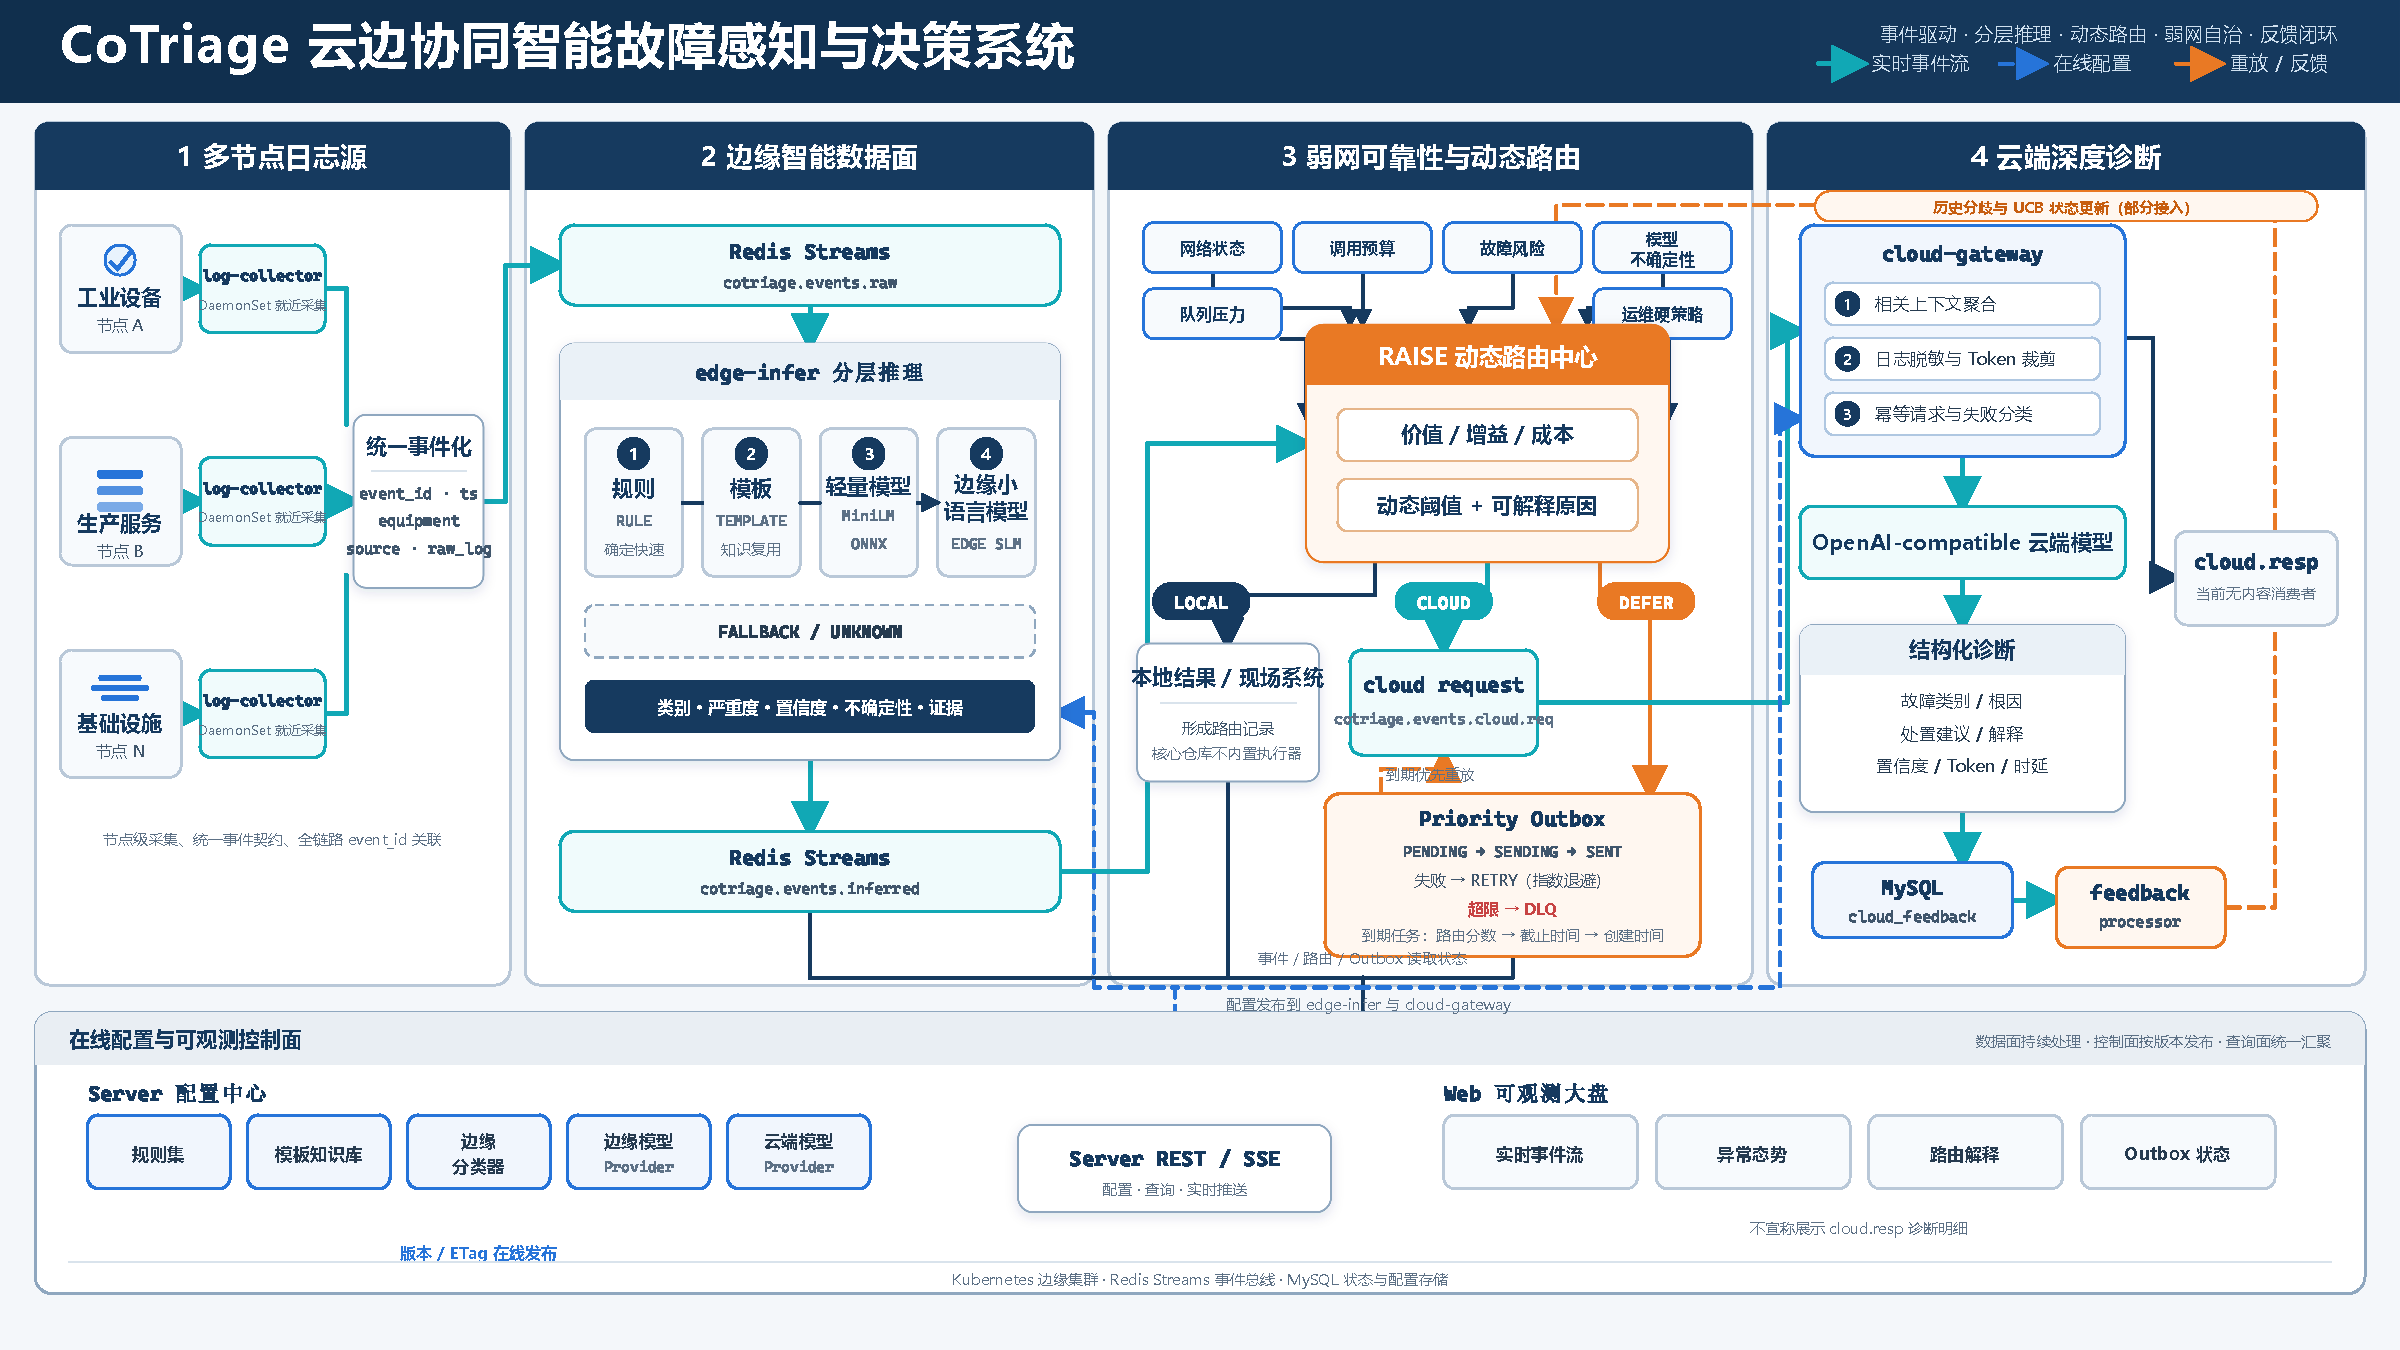
\includegraphics[width=\textwidth]{figures/cotriage-system-architecture.pdf}
  \caption{CoTriage 云—边—端协同总体架构}
  \label{fig:architecture}
\end{figure}

\cref{fig:architecture}从左至右描述了一条事件如何跨层流动。端侧多个日志源由近端采集器转换为统一事件；边缘侧通过 Redis Streams 解耦持续事件流，依次完成异构分层推理和 RAISE 路由，确定性事件在本地闭环，高价值事件进入云端请求流，暂不可发送的事件进入风险优先 Outbox；云端网关裁剪并脱敏上下文，调用兼容 Provider 生成根因、建议和解释，再把结果持久化并形成反馈。Server 与 Web 组成统一控制和观测入口，贯穿三层但不阻塞后台数据面。

架构中的“协同”体现在三个方面。其一是\textbf{能力协同}：规则、模板、轻量模型、边缘小模型与云端大模型按事件难度逐级使用。其二是\textbf{资源协同}：网络、队列、预算和策略直接进入路由判断，避免云端能力被当作无限资源。其三是\textbf{时间协同}：实时结果与深度结果可以异步产生，Outbox 又把“当前不能发送”转换为“条件恢复后继续分析”，使诊断深度不必与现场响应共用同一时限。

\section{端侧：多源日志感知与可信事件生成}

端侧包括工业设备控制程序、工控机操作系统、Linux 主机、Hadoop 或 ZooKeeper 节点以及 Web 服务等日志产生单元。不同来源的文本格式和业务语义可以不同，但进入协同主链前必须获得共同坐标：稳定事件标识、设备标识、来源、采集时间和原始内容。\texttt{log-collector} 以节点近端方式持续读取新增日志，尽快完成事件化并写入原始事件流，不在采集阶段执行高成本语义判断。

将采集能力放在端侧附近具有三项作用。第一，日志在产生后无需等待跨网传输即可进入处理链，降低现场感知对外部网络的依赖；第二，设备身份在源头绑定，后续跨节点关联不必仅靠正文猜测来源；第三，原始日志可以优先留在边缘域，只有被选中的事件及裁剪上下文才需要跨越云边边界。端侧的职责是持续、轻量、忠实地提供证据，而不是独立完成所有诊断。

端侧发生故障时，系统采用“局部影响、恢复续接”的原则：单个采集实例异常不应阻塞其他节点，恢复后继续读取新增内容；日志来源新增时只扩展采集适配与设备登记，不改变上游推理和路由契约。第 4 章将进一步说明多节点登记、统一事件字段、消息确认与幂等追踪。

\section{边缘侧：实时推理、价值路由与弱网自治}

边缘侧是 CoTriage 的实时决策中心，而不是云端模型的简单转发代理。它部署在工厂、园区或站点近端，由事件总线、\texttt{edge-infer}、\texttt{onnx-classifier}、\texttt{router-controller} 和 Outbox 共同组成，承担“先形成可用判断，再决定是否需要更强能力”的职责。

\subsection{由快到慢的现场推理链}

\texttt{edge-infer} 将规则、模板知识库、MiniLM ONNX 轻量分类器和边缘小语言模型组织为可早停的分层路径。明确告警优先由规则或模板低成本收敛，常见但未命中的语义交给轻量模型，开放性更强的内容再调用边缘小模型。各层输出统一的类别、严重度、置信度、不确定性、证据、推理路径和版本，使后续路由不依赖某一种模型的私有格式。某一模型不可用时，系统保留上一层有效判断并显式记录降级，而不是把服务故障误判为日志正常。

\subsection{RAISE 事件级路由}

边缘推理得到的“当前判断”并不直接等同于最终处理位置。\texttt{router-controller} 通过 RAISE 分离两个问题：事件是否值得获得云端增益，以及此刻是否具备发送条件。前者由风险、不确定性、新颖度、历史边云分歧与跨设备影响共同描述，后者由网络健康、队列压力、调用预算、限流、隐私和运维策略约束。控制器据此输出 \texttt{LOCAL}、\texttt{CLOUD} 或 \texttt{DEFER}，并保存分数、动态门槛、原因和系统快照。

\subsection{弱网条件下的连续运行}

\texttt{LOCAL} 事件直接形成可供现场系统消费的结果；\texttt{CLOUD} 事件进入云端请求流；\texttt{DEFER} 事件先写入 MySQL Outbox，按风险优先级和到期时间重试，超过边界后进入死信治理。由此，断网不会阻塞端—边实时闭环，高价值事件也不会因为一次发送失败永久失去深诊机会。Redis Streams 的追加日志和消费组机制用于解耦边缘各阶段\cite{redisstreams}，MySQL 则保存需要跨重启恢复的路由、Outbox 和状态快照。

\section{云端：跨节点上下文与大模型深度诊断}

云端只接收边缘选择出的高价值事件，不承担全量原始日志的同步处理。\texttt{cloud-gateway} 以主事件为中心，从可用事件中筛选时间邻近、同源、同模板和跨设备关联上下文，对主日志与关联原文执行脱敏，并在 Token 预算内构造诊断请求。云端 Provider 通过 OpenAI-compatible 接口按需接入，使模型可以替换而不改变边缘事件与路由契约。

云端目标不是再次输出一个分类标签，而是把全局信息增量转化为结构化结果：根因候选回答最可能的故障起点，处置建议给出优先检查和操作方向，诊断解释说明采用了哪些现象与关联证据。结果以事件标识和幂等键持久化，避免重试产生重复高成本调用；随后形成纠错、信息增量或高风险确认等反馈，写回事件状态与在线统计，为后续策略演进提供依据。

Server 与 Web 主要部署在中心控制域，提供 REST/SSE、设备和模型配置、运行状态查询与可视化。控制面可以改变规则、模板、模型 Provider 和运维策略，观测面可以展示实时事件、异常态势、路由解释、Outbox 和诊断结果，但两者短时不可用不应停止端侧采集与边缘处理。云端因而同时承担“深度智能中心”和“统一治理中心”两种角色，二者通过接口与实时数据面解耦。

\section{跨层协同：数据流、控制流与反馈流}

云—边—端架构要稳定运行，仅有一条向上的日志流并不够。CoTriage 将跨层通信划分为三类方向不同、时限不同的通道，避免管理操作、实时事件与模型反馈相互阻塞。

\begin{table}[htbp]
  \centering
  \small
  \caption{云、边、端之间的三类协同通道}
  \label{tab:cross-layer-flows}
  \begin{tabularx}{\textwidth}{>{\bfseries}p{0.15\textwidth} p{0.19\textwidth} X X}
    \toprule
    通道 & 主要方向 & 承载内容 & 时限与失败处理 \\
    \midrule
    实时数据流 & 端侧 $\rightarrow$ 边缘侧 & 原始事件、推理事件、本地结果和路由记录 & 持续处理；云端故障不得阻塞端—边主链 \\
    按需诊断流 & 边缘侧 $\leftrightarrow$ 云端 & 已选事件、裁剪上下文、结构化诊断与反馈 & 异步完成；发送受限时进入 Outbox，调用幂等 \\
    控制与观测流 & 云端 $\leftrightarrow$ 边缘／端侧 & 设备、规则、模板、模型、策略、健康与运行状态 & 配置原子生效；失败沿用上一有效版本，观测中断不影响数据面 \\
    \bottomrule
  \end{tabularx}
\end{table}

统一事件是三类通道之间的公共语言。事件标识串联原文、推理、路由和诊断，幂等键约束跨层重试的副作用，规则与模型版本说明当时使用了哪一份能力，路由快照则保留当时的网络、队列、预算与门槛。系统由此不仅能回答“结果是什么”，还能还原“哪一层做了什么、为什么跨层、失败后如何继续”。

\section{端到端事件闭环与部署边界}

一条事件在端侧生成后进入 \texttt{CREATED}，完成边缘推理后转为 \texttt{INFERRED}，形成 RAISE 动作后进入 \texttt{ROUTED}。\texttt{LOCAL} 在边缘结束实时链路；\texttt{CLOUD} 进入云端深诊；\texttt{DEFER} 先进入 Outbox，条件满足后再上云。云端响应最终与原事件关联，并写回诊断与反馈状态。这个生命周期允许事件早停、异步补充和失败重试，不要求所有日志经过完全相同的计算路径。

\begin{table}[htbp]
  \centering
  \footnotesize
  \caption{主要组件在云—边—端架构中的部署与扩展方式}
  \label{tab:layered-components}
  \begin{tabularx}{\textwidth}{>{\bfseries}p{0.10\textwidth} >{\ttfamily}p{0.20\textwidth} X X}
    \toprule
    层级 & \normalfont\bfseries 组件 & 典型部署方式 & 独立扩展依据 \\
    \midrule
    端侧 & log-collector & 按节点部署，生产环境可采用 DaemonSet 或独立采集进程 & 日志来源数量与单节点产生速率 \\
    边缘 & edge-infer / onnx-classifier & 站点近端 Deployment 或本地模型服务 & 事件吞吐、模型时延与边缘资源 \\
    边缘 & router-controller & 独立持续处理组件，连接 Redis 与 MySQL & 路由吞吐、Outbox 规模与重试压力 \\
    云端 & cloud-gateway & 独立 Deployment，通过兼容接口访问 Provider & 云端并发、限流、Token 与预算 \\
    云端 & server / web & 控制与查询服务、Web 服务 & API、SSE 连接和管理访问量 \\
    \bottomrule
  \end{tabularx}
\end{table}

各组件通过统一事件、Redis Streams、HTTP 和 MySQL 状态协作，并可由 Kubernetes 执行声明式部署与独立扩缩容\cite{kubernetes}。当前实现边界也保持明确：\texttt{LOCAL} 结果提供给外部现场系统消费，仓库不内置真实生产处置执行器；Outbox 采用到期扫描重放，尚未由网络恢复信号直接触发；云端反馈已进入统计和状态快照，学习增益尚未自动改写在线路由评分。明确这些边界既避免把演示能力夸大为生产闭环，也为后续工程化提供清晰方向。

后续章节将沿云—边—端主链逐层展开：第 4 章说明端侧多节点采集与统一事件化，第 5 至第 6 章说明边缘分层推理、RAISE 与弱网补偿，第 7 章说明云端上下文诊断和反馈闭环，第 8 章说明统一治理与产品化展示。

\chapter{多节点采集与统一事件化}

\section{节点近端持续采集}
\texttt{log-collector} 以节点近端部署方式持续读取日志新增内容。它不尝试在采集阶段完成复杂语义判断，而是尽快把一行原始日志转换为带来源、设备和时间信息的事件并写入原始事件流。这样可以把“日志产生速度”与“后续推理复杂度”解耦：采集器保持轻量，推理层则可以独立扩展实例或更换模型。

采集靠近数据源还有两项直接价值。第一，边缘快速路径不需要等待跨网传输；第二，原始日志可以优先留在边缘域，只有被路由选中的事件及裁剪后的上下文才进入云端。当前采集器按非空日志行事件化，时间窗口聚合、日志轮转与 inode 切换属于进一步增强项。

\section{多类节点的统一登记与接入状态}

在多节点采集开始前，管理端以统一设备记录维护节点标识、设备名称和就绪状态，使后续事件能够关联到稳定来源，而不依赖日志正文临时推断设备身份。Apache、Linux、Hadoop 和 ZooKeeper 等不同类型的日志源使用同一登记接口进入系统；采集适配可以因来源而变化，但节点状态查询、事件标识和后续处理契约保持一致。

\begin{figure}[htbp]
  \centering
  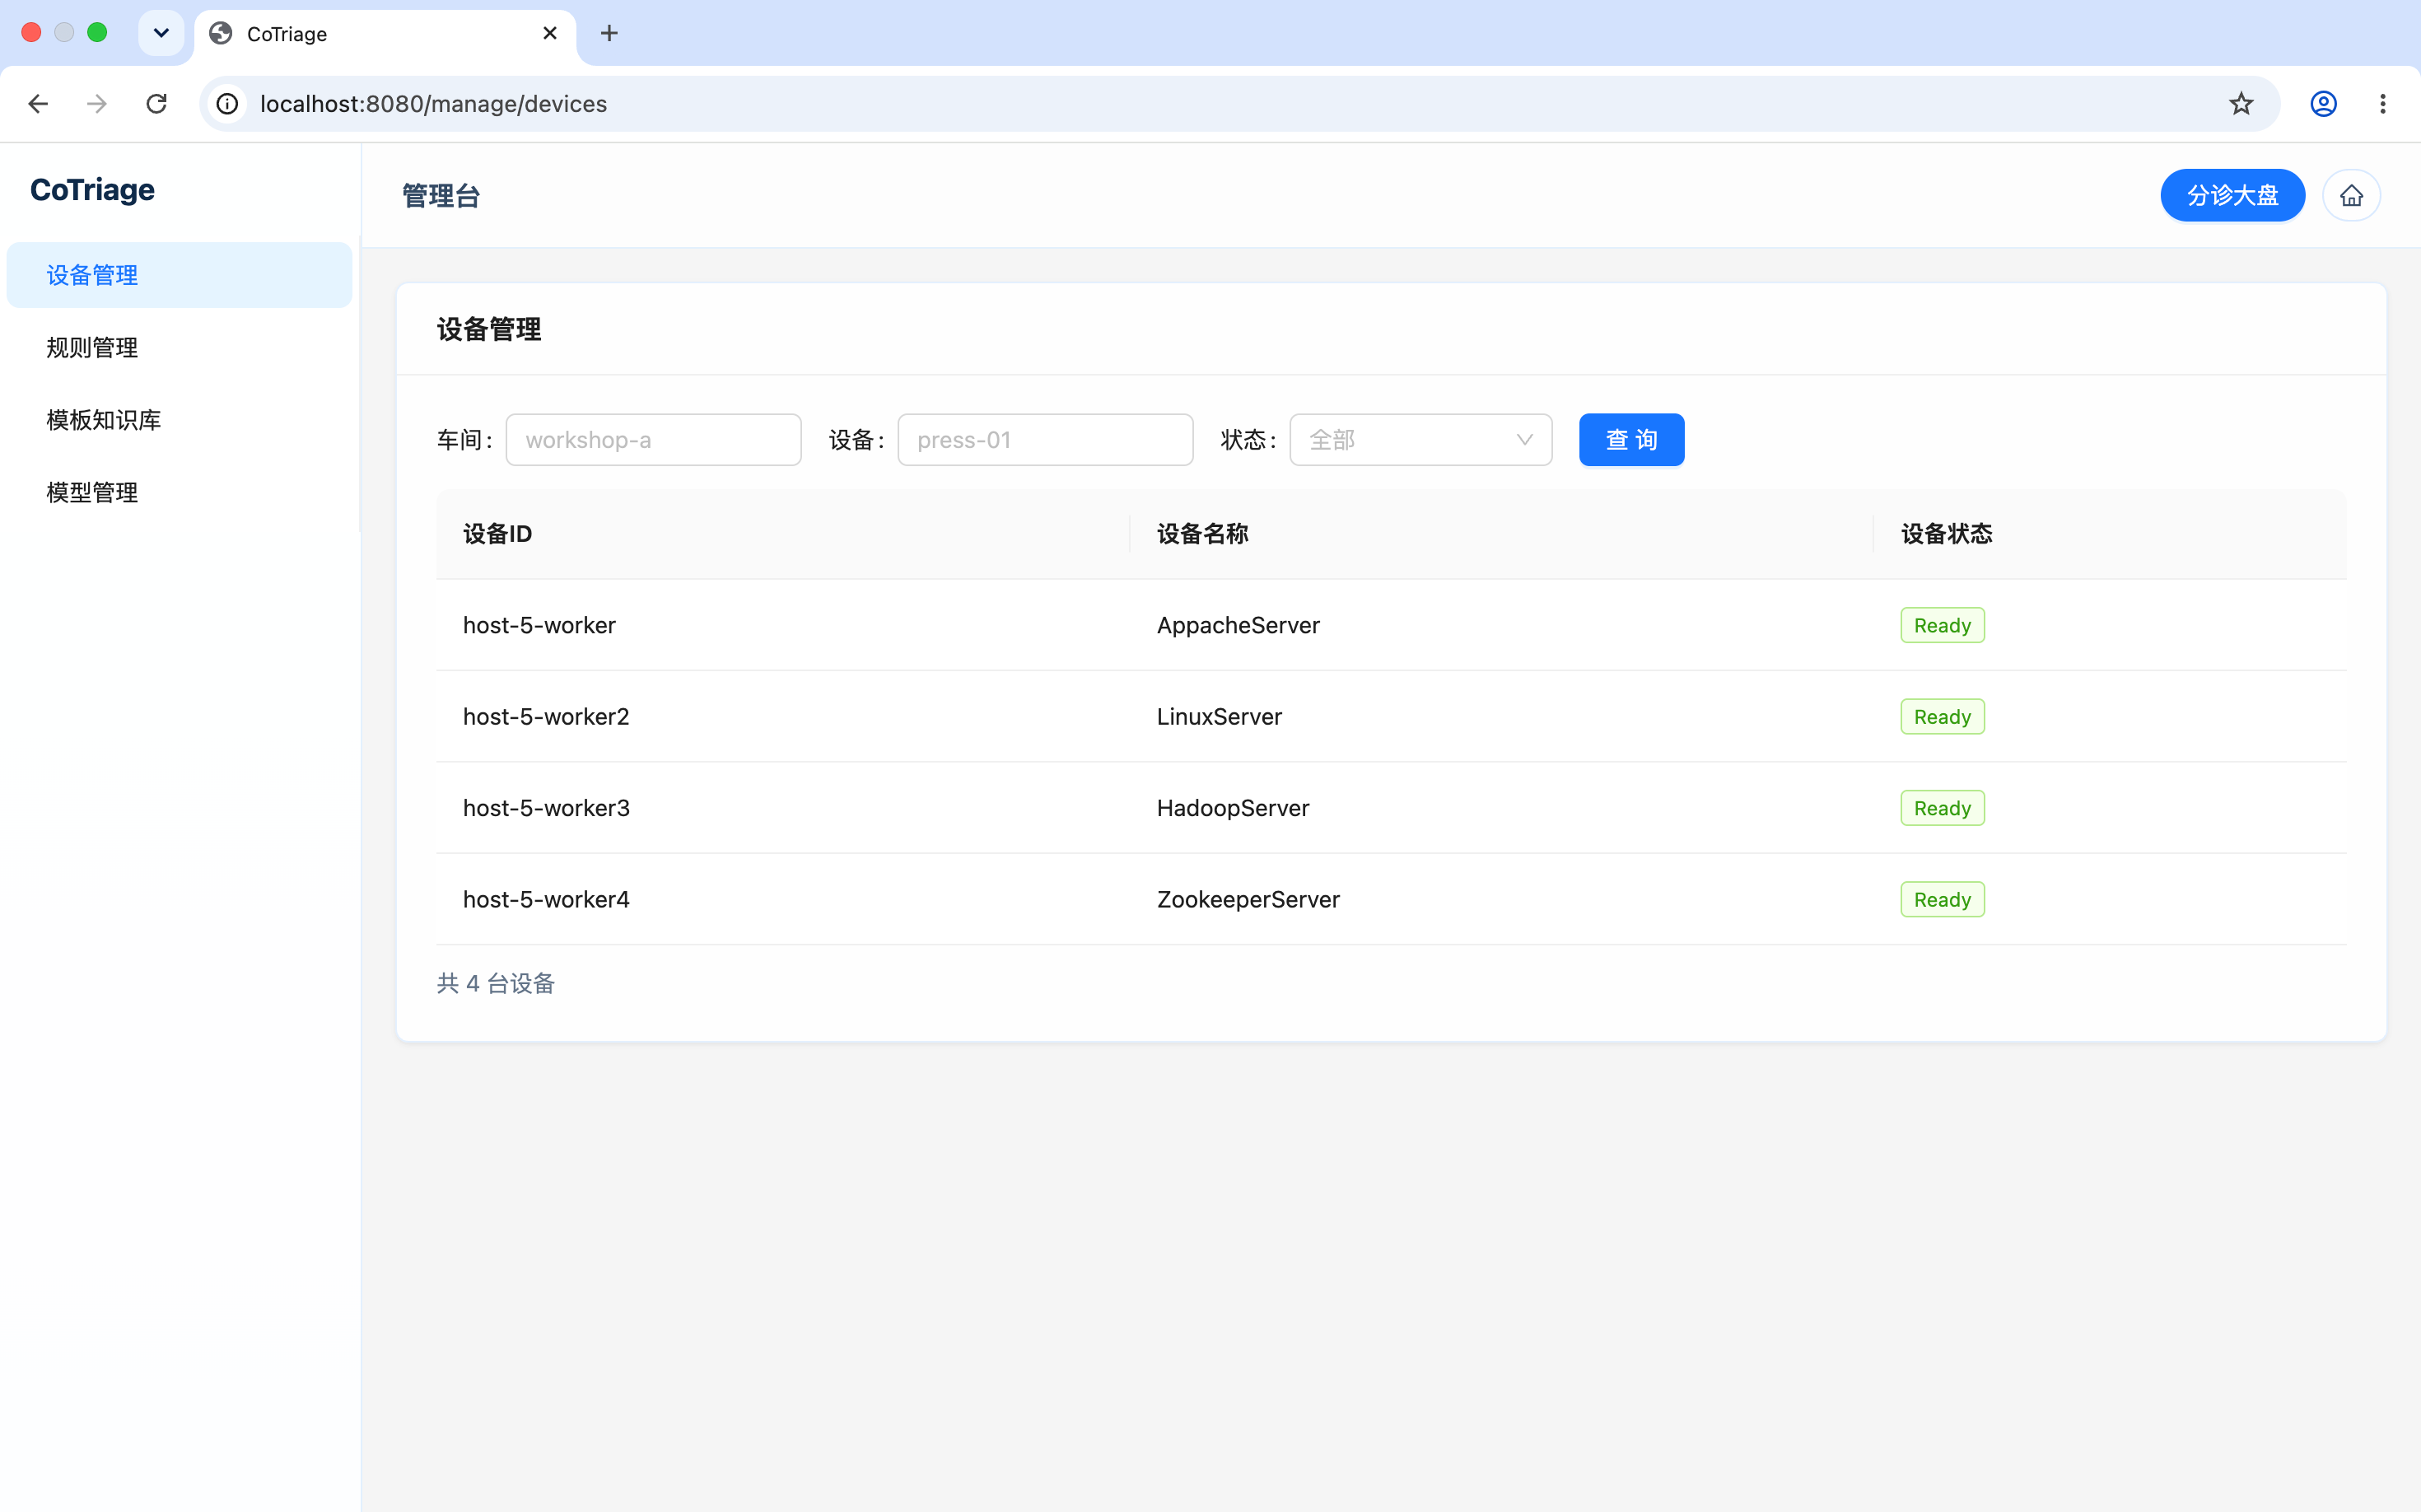
\includegraphics[width=0.90\textwidth]{figures/s-02-device-management.png}
  \caption{多类日志节点在管理端统一登记并呈现就绪状态}
  \label{fig:device-management}
\end{figure}

\cref{fig:device-management}展示了当前运行环境中的多类节点登记结果。该页面一方面验证采集链能够区分不同设备与日志来源，另一方面为事件流中的设备筛选、跨节点上下文聚合和运行状态下钻提供入口。图中数量仅反映截图时的登记情况，不用于推断系统扩展上限；节点规模变化主要由采集实例、Stream 消费组和后续处理服务的独立扩容承接。

\section{统一事件模型}
统一事件不是修改原始日志含义，而是在原文之外增加可跨组件复用的公共字段。核心字段分为四组。

\begin{table}[htbp]
  \centering
  \small
  \caption{统一事件的字段分组及其作用}
  \label{tab:event-fields}
  \begin{tabularx}{\textwidth}{>{\bfseries}p{0.17\textwidth} p{0.29\textwidth} X}
    \toprule
    字段组 & 代表字段 & 作用 \\
    \midrule
    身份与来源 & \texttt{event\_id}、设备、来源、时间 & 跨节点区分事件并支持时间排序 \\
    原始内容 & 原始日志、归一化模板、上下文摘要 & 保留诊断信息并支持模板复用 \\
    推理结果 & 类别、严重度、置信度、不确定性、路径、版本、时延 & 说明边缘如何形成当前判断 \\
    路由与状态 & 动作、分数、阈值、原因、预算、网络、队列快照 & 说明为何选择本地、云端或延期 \\
    \bottomrule
  \end{tabularx}
\end{table}

稳定的事件契约使规则引擎、模型服务和 Web 页面可以独立演进。即使某次判断更换了模型，\texttt{event\_id} 与版本字段仍能把该事件的原文、推理、路由和云端结果串联起来。

\section{实时事件流与推理路径}
\begin{figure}[htbp]
  \centering
  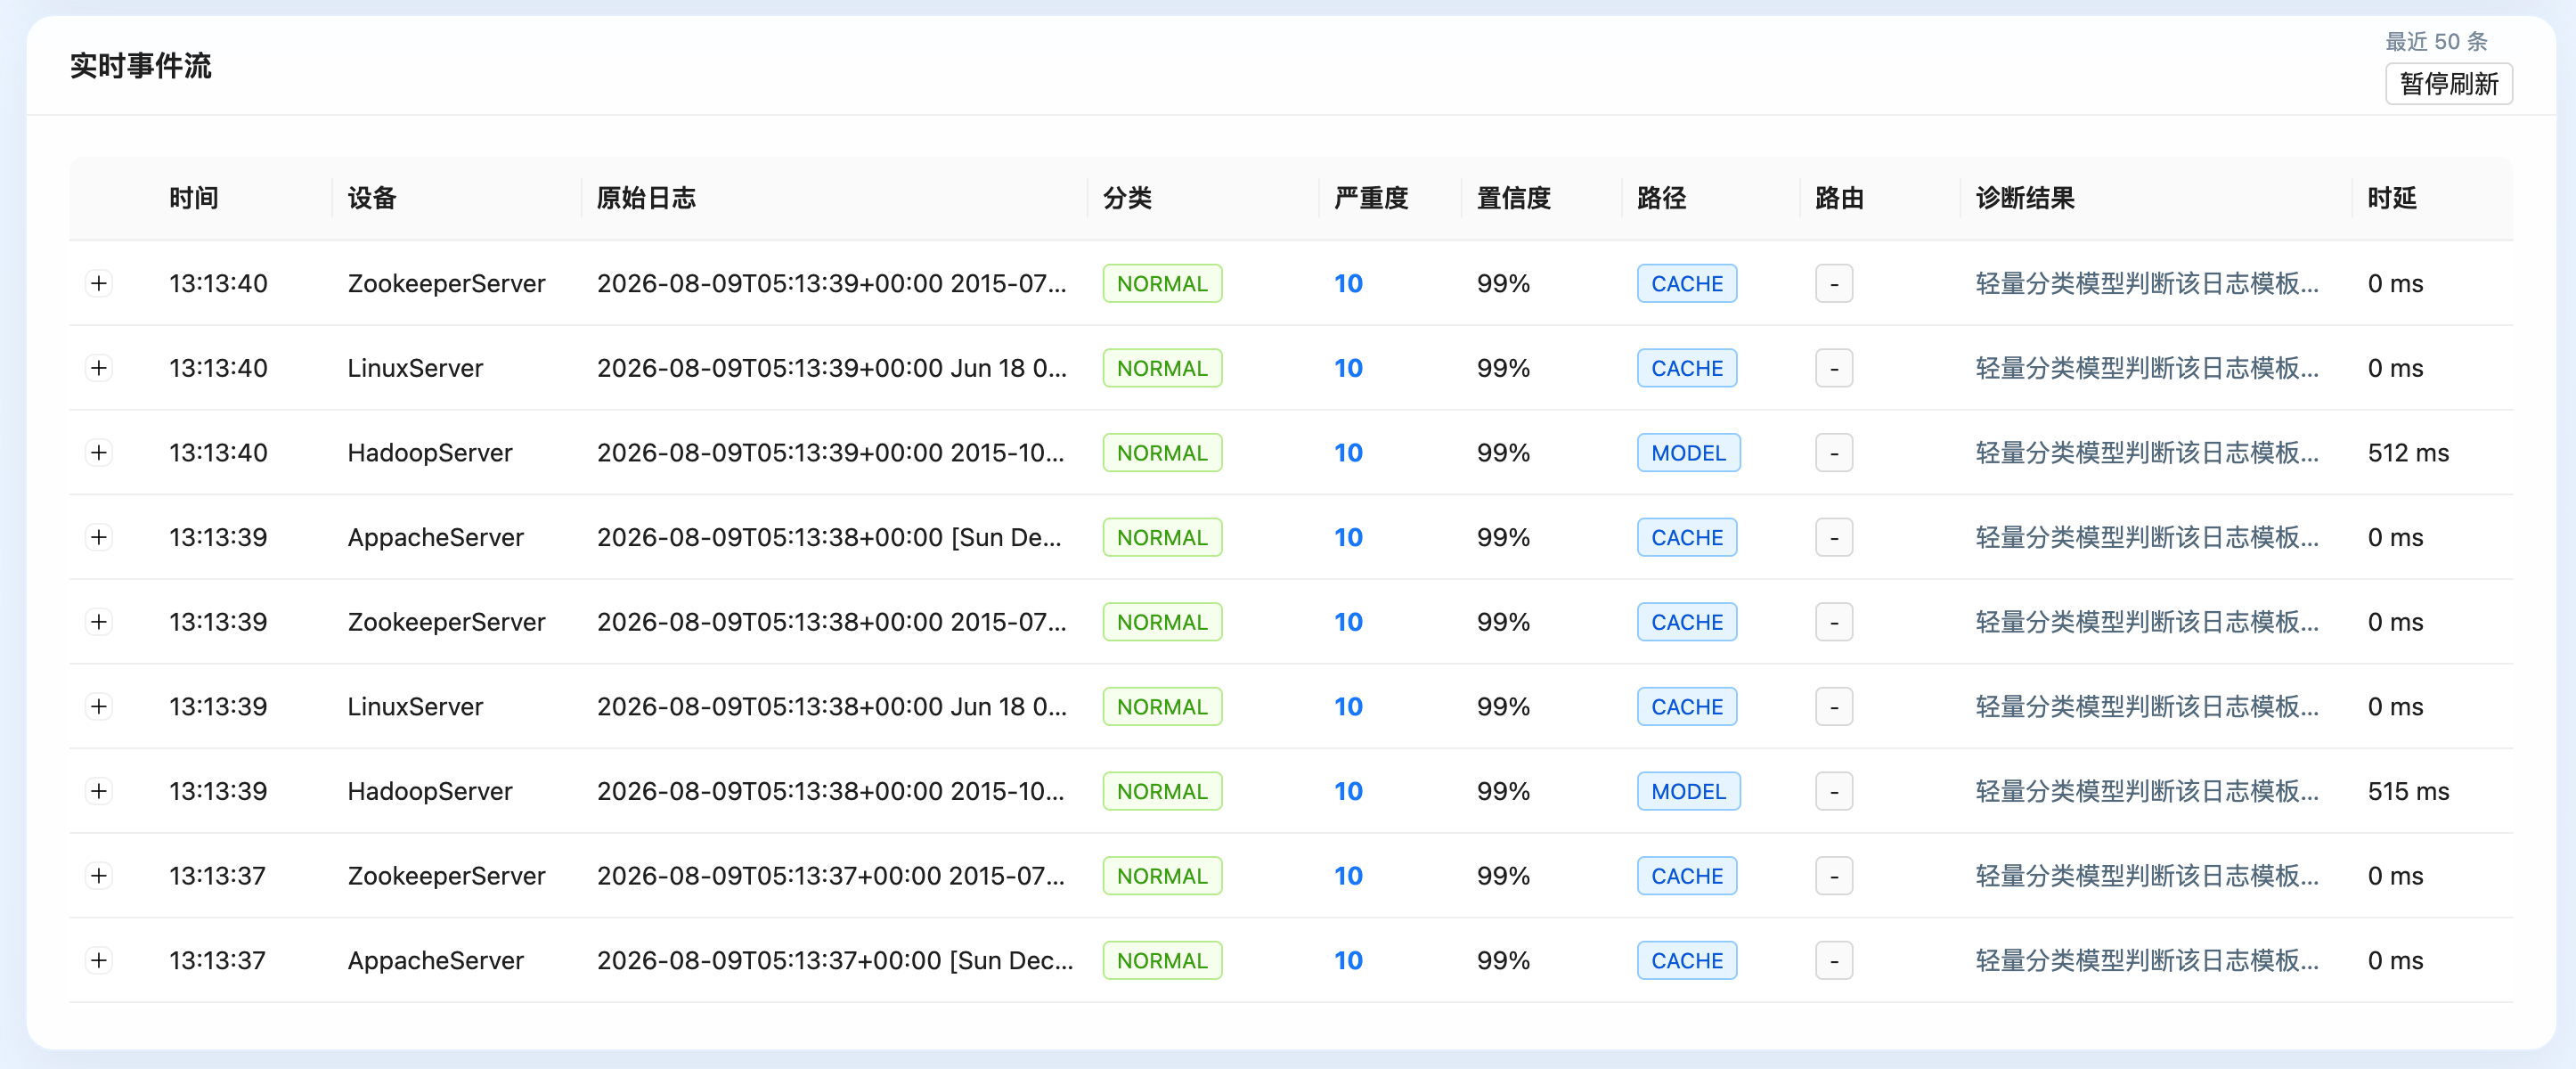
\includegraphics[width=0.98\textwidth]{figures/s-02d-realtime-event-stream-cache-model.png}
  \caption{统一事件流同时呈现不同设备与边缘推理路径}
  \label{fig:event-stream-cache-model}
\end{figure}

\cref{fig:event-stream-cache-model}在同一页面中展示了多个设备的原始日志、类别、严重度、置信度、推理路径、路由字段、诊断摘要和单事件耗时。画面中的 \texttt{CACHE} 与 \texttt{MODEL} 表明事件可以在不同边缘层级结束；表内耗时是各事件当次处理记录，不应直接替代运行窗口的平均值或 P95 指标。

\section{消息确认、幂等与追踪}
原始事件、推理结果、路由结果和云端请求分别进入独立 Stream。Consumer Group 让多个实例分担消费，ACK 表示消息已经完成当前阶段；已投递但未确认的消息进入 Pending Entries List。边缘推理已具备 Pending 接管机制，路由与云端网关仍需进一步统一接管策略。

系统将延迟确认和幂等组合使用：先完成持久化与下游发布，再确认当前消息；重试时依据幂等键复用既有状态，避免重复产生高成本调用。推理路径、模型版本、规则版本、时延和路由快照则进入观测面，使运维人员能够从驾驶舱下钻到单事件处理过程。

\section{从日志行到可操作事件}
一次完整处理可以概括为五步：采集器读取日志并生成唯一标识；边缘推理补充类别、风险与路径；RAISE 结合系统状态产生动作和解释；被选中的事件进入云端上下文聚合；最终结果通过数据库、消息流和 Web 页面被保存和展示。统一事件是这五步之间的公共语言，也是后续场景扩展和问题复盘的最小单位。

\chapter{边缘分层推理与在线配置}

\section{由快到慢的四级路径}
边缘侧把规则、模板知识库、MiniLM ONNX 轻量分类器和边缘小语言模型组织为由快到慢、由确定到开放的处理路径。这里的“分层”并不意味着每条日志都依次调用四种方法，而是允许事件在信息已经足够时提前结束，把有限算力留给更难的事件。

\begin{enumerate}
  \item \textbf{规则层：}识别磁盘不足、认证失败、连接错误等明确模式，响应快、解释直接；
  \item \textbf{模板层：}复用重复日志模板及其历史结论，减少相似事件的重复计算；
  \item \textbf{轻量模型层：}通过 MiniLM ONNX 服务覆盖规则和模板之外的常见语义；
  \item \textbf{边缘小语言模型层：}对需要开放语义解释、但仍适合在现场处理的事件补充判断。
\end{enumerate}

若轻量模型未配置或调用失败，系统进入显式 \texttt{FALLBACK/UNKNOWN}；若轻量模型已经成功输出而边缘小语言模型失败，则保留现有 \texttt{MODEL} 结果并附加错误信息，不把已有判断改写为未知。明确的降级语义能够避免“模型不可用”被误解为“日志正常”。

\section{推理输出契约}
每次边缘推理输出类别、严重度、置信度、不确定性、推理路径、解释信息、模型版本、规则版本、模板集版本和处理时延。置信度描述模型对当前输出的把握，不确定性则作为 RAISE 的风险信号；二者都不能脱离任务、数据和统计口径直接解释为“判断正确的概率”。

MiniLM 采用 ONNX 作为训练侧与 Go 主链之间的稳定部署接口。模型服务通过本地 HTTP 返回结果，业务组件不需要理解训练框架内部结构。轻量语义表示的基础方法与 Sentence-BERT 类工作相关\cite{reimers2019sentencebert}，当前部署任务聚焦日志告警初筛。

\section{运行趋势与路径分布}
\begin{figure}[htbp]
  \centering
  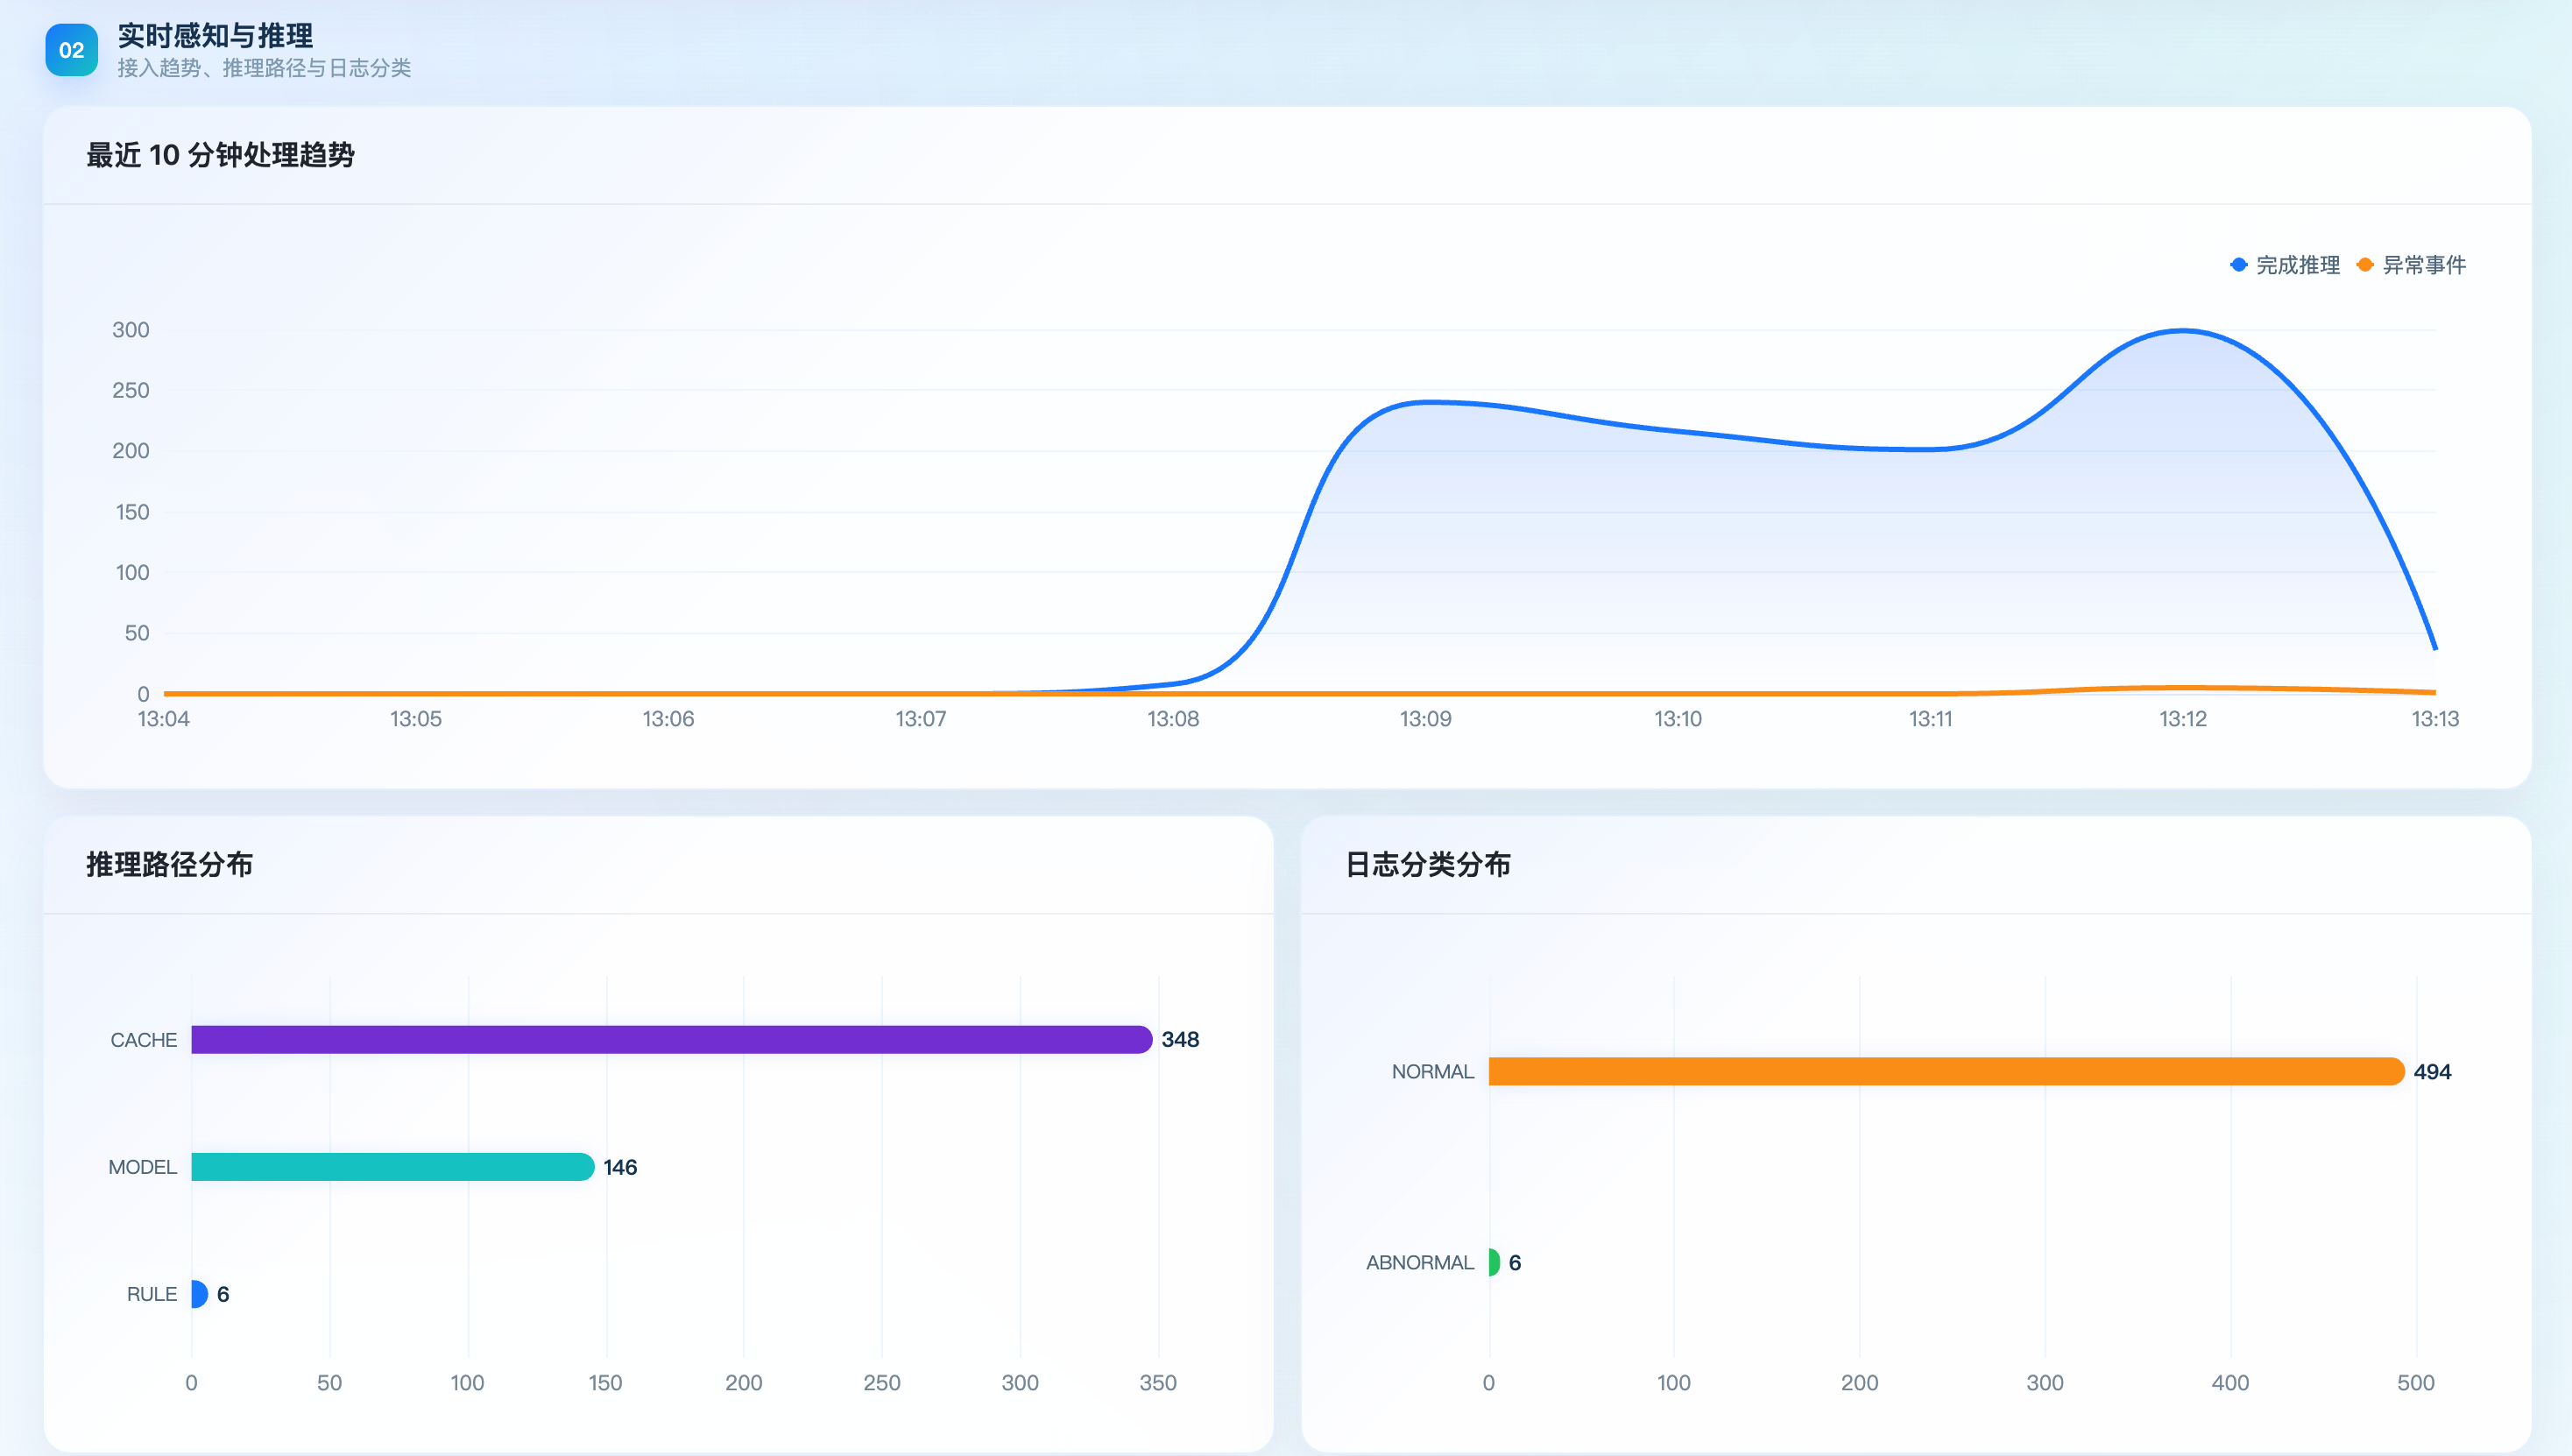
\includegraphics[width=0.98\textwidth]{figures/s-02c-inference-trend-and-distribution.png}
  \caption{当前运行窗口的处理趋势、推理路径与日志类别分布}
  \label{fig:inference-trend}
\end{figure}

\cref{fig:inference-trend}把最近十分钟的处理趋势与 \texttt{CACHE/MODEL/RULE} 路径分布放在同一观察面中。它能够直观说明分层推理在运行时确实存在不同早停路径，并帮助运维人员发现异常比例或某类推理路径的突变。图中数量属于截图对应的运行窗口，不用于推导长期业务比例。

\begin{figure}[htbp]
  \centering
  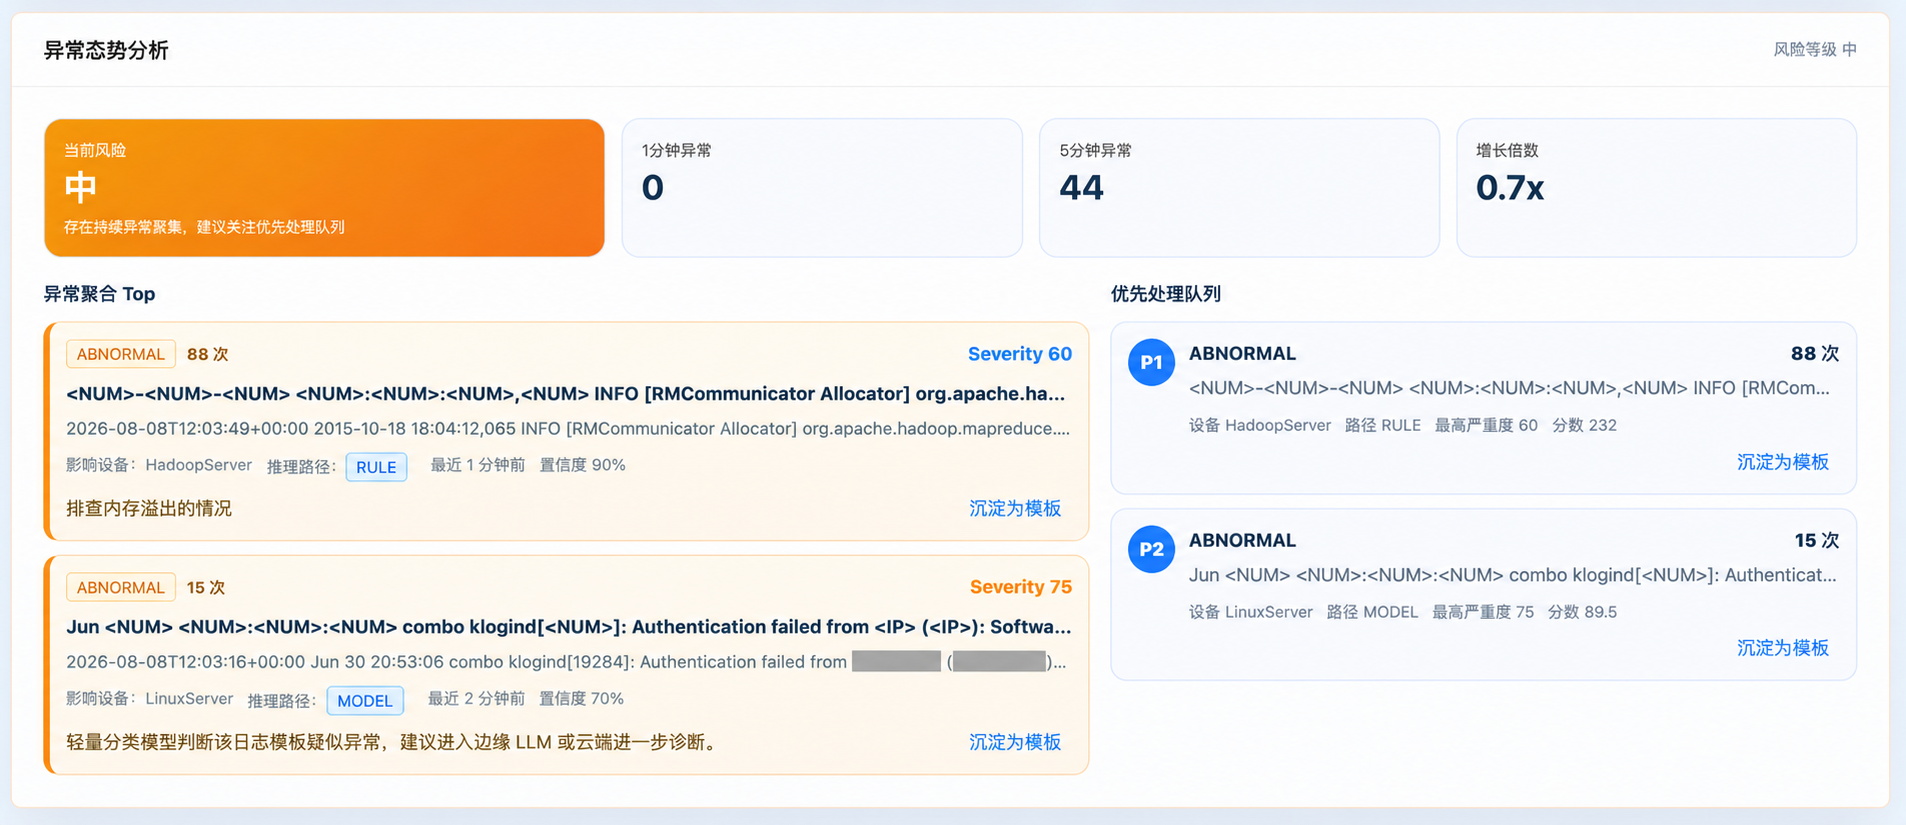
\includegraphics[width=0.98\textwidth]{figures/s-03-anomaly-trend-analysis-redacted.png}
  \caption{历史日志回放中的异常聚合与优先处理队列}
  \label{fig:anomaly-analysis}
\end{figure}

\cref{fig:anomaly-analysis}展示了异常模板聚合、风险等级和优先处理队列。该页面基于脱敏后的历史日志样本回放，用于说明系统如何把分散事件组织成运维可读的异常态势，不将其描述为真实生产事故。

\section{规则与模型在线治理}
规则、模板和模型配置由 Server 发布，\texttt{edge-infer} 使用 ETag 轮询。完整响应会先完成解析与校验；校验失败时继续使用上一份有效配置，校验通过后再更新知识和模型子系统。ETag 相当于配置内容的版本指纹：内容未变化时不重复传输，内容变化时才触发更新。

\begin{figure}[htbp]
  \centering
  \begin{subfigure}[t]{0.49\textwidth}
    \centering
    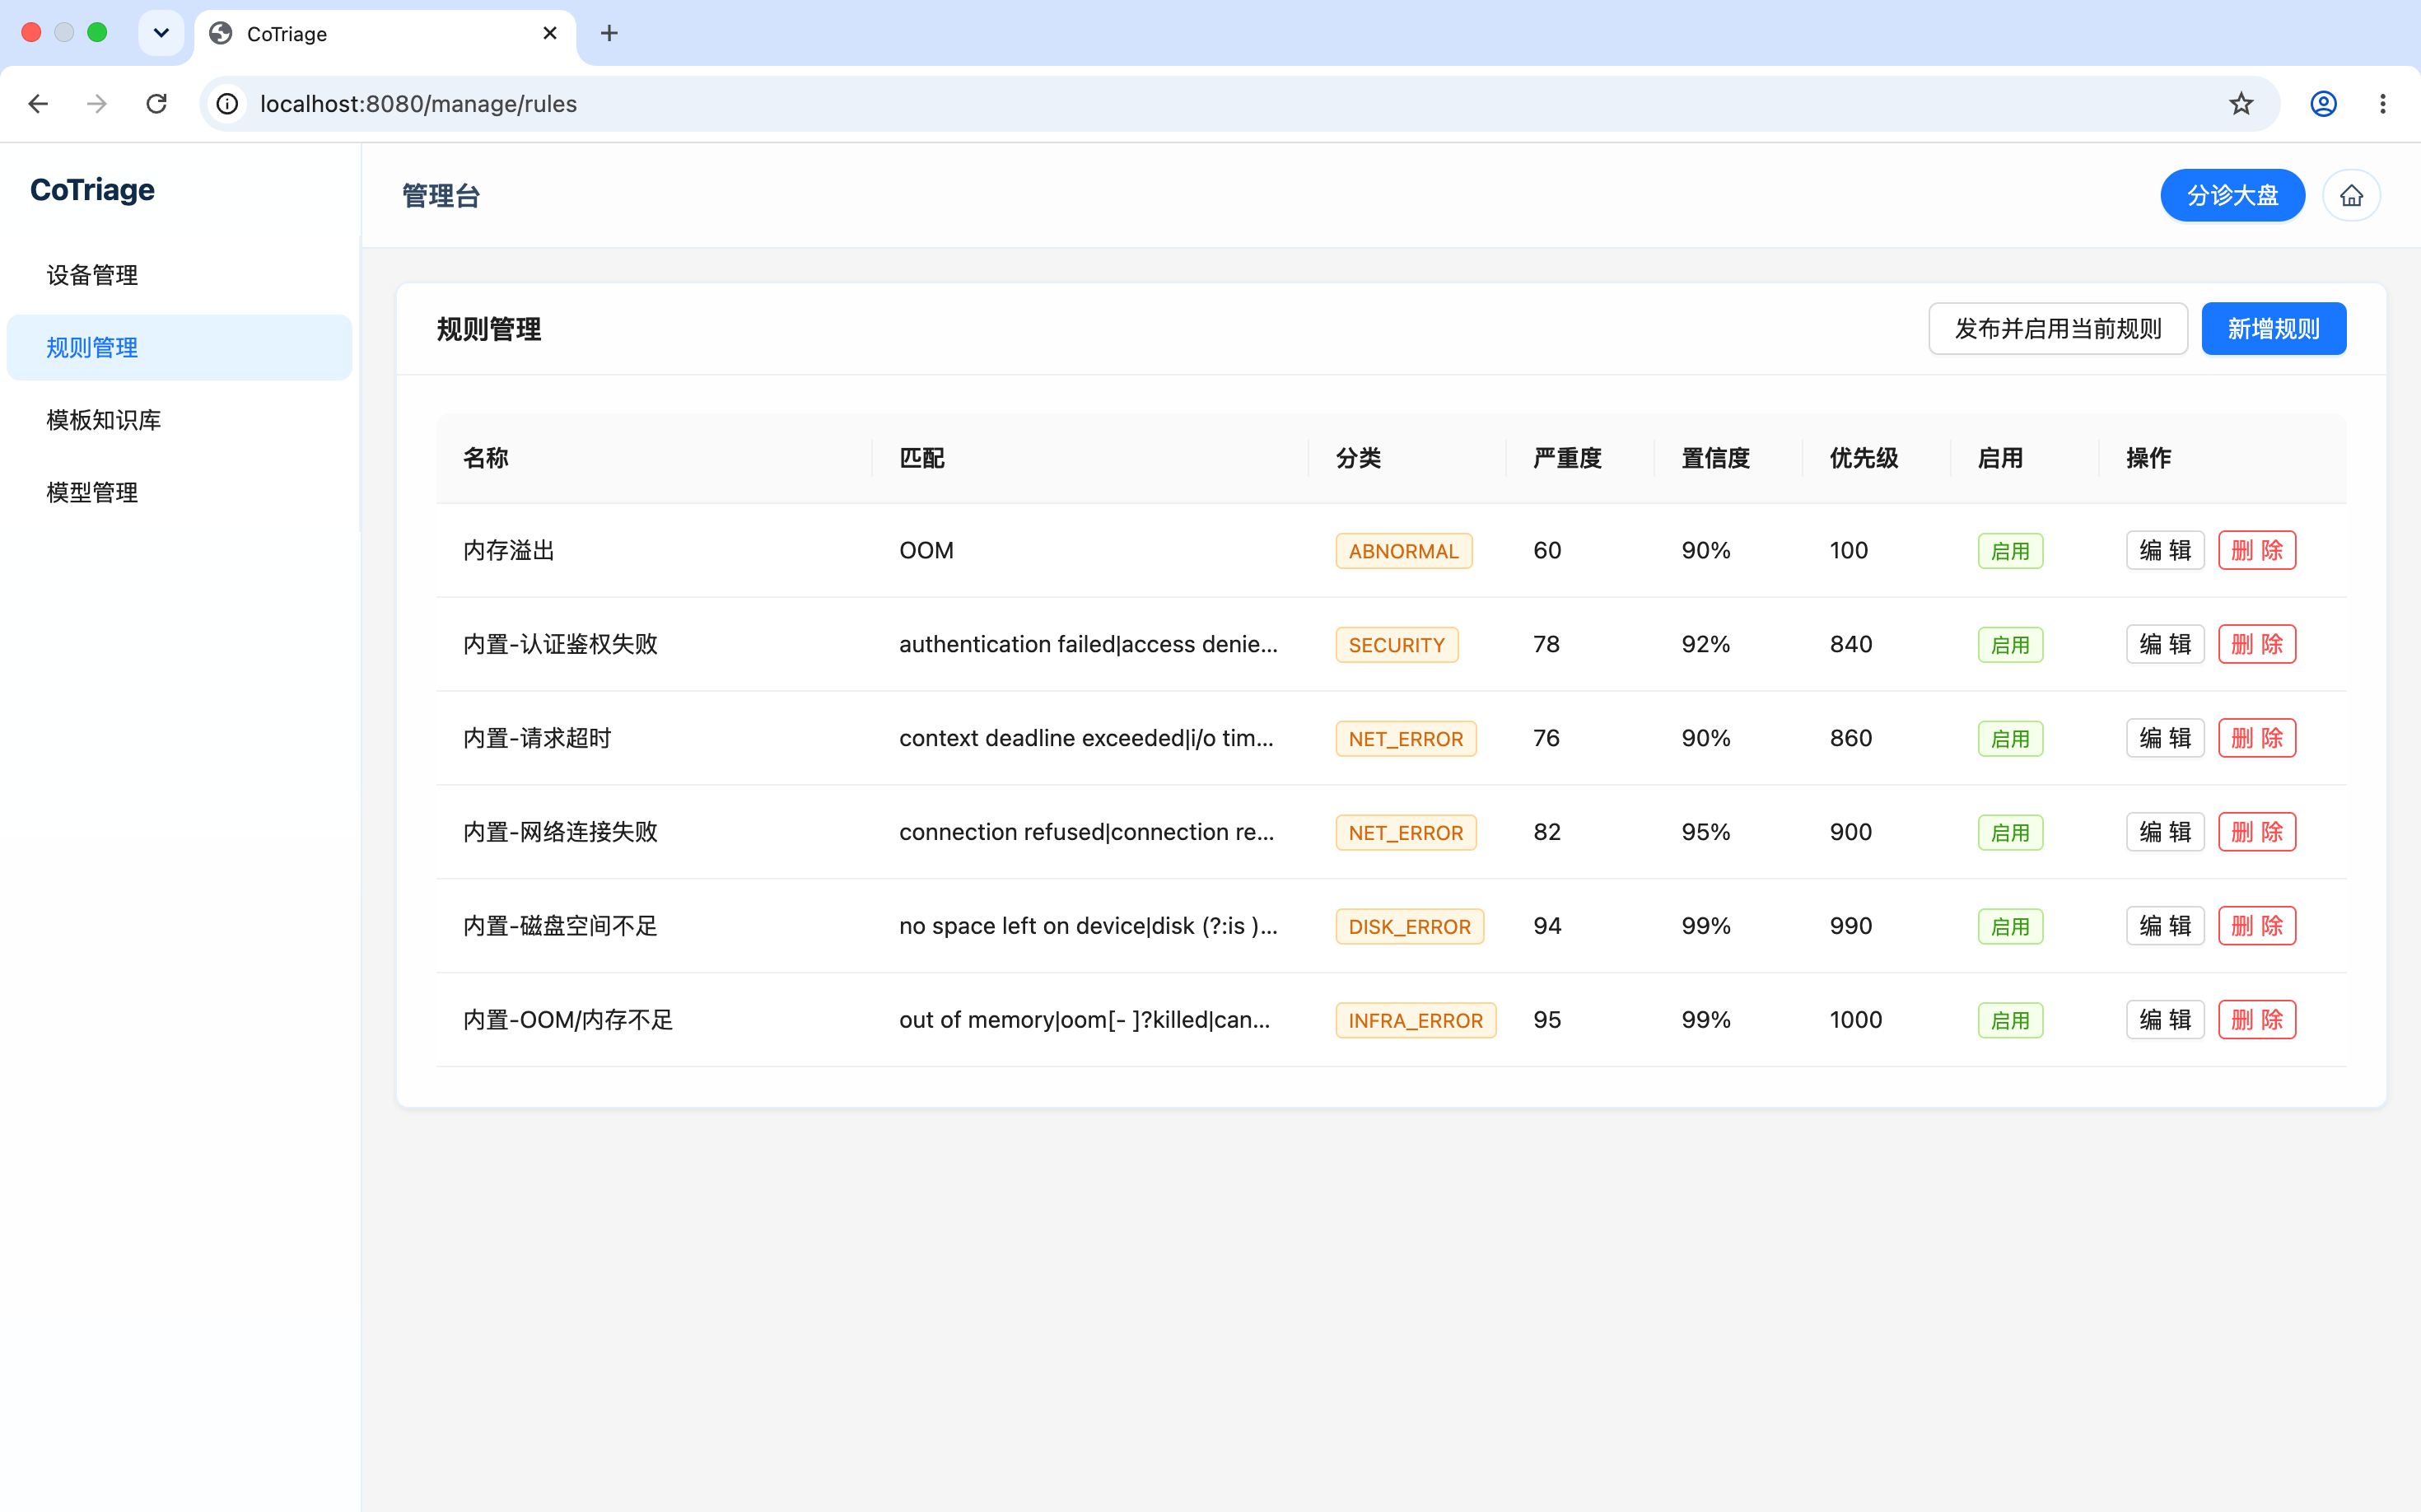
\includegraphics[width=\linewidth]{figures/s-08a-rule-management.png}
    \caption{规则发布与启用}
  \end{subfigure}\hfill
  \begin{subfigure}[t]{0.49\textwidth}
    \centering
    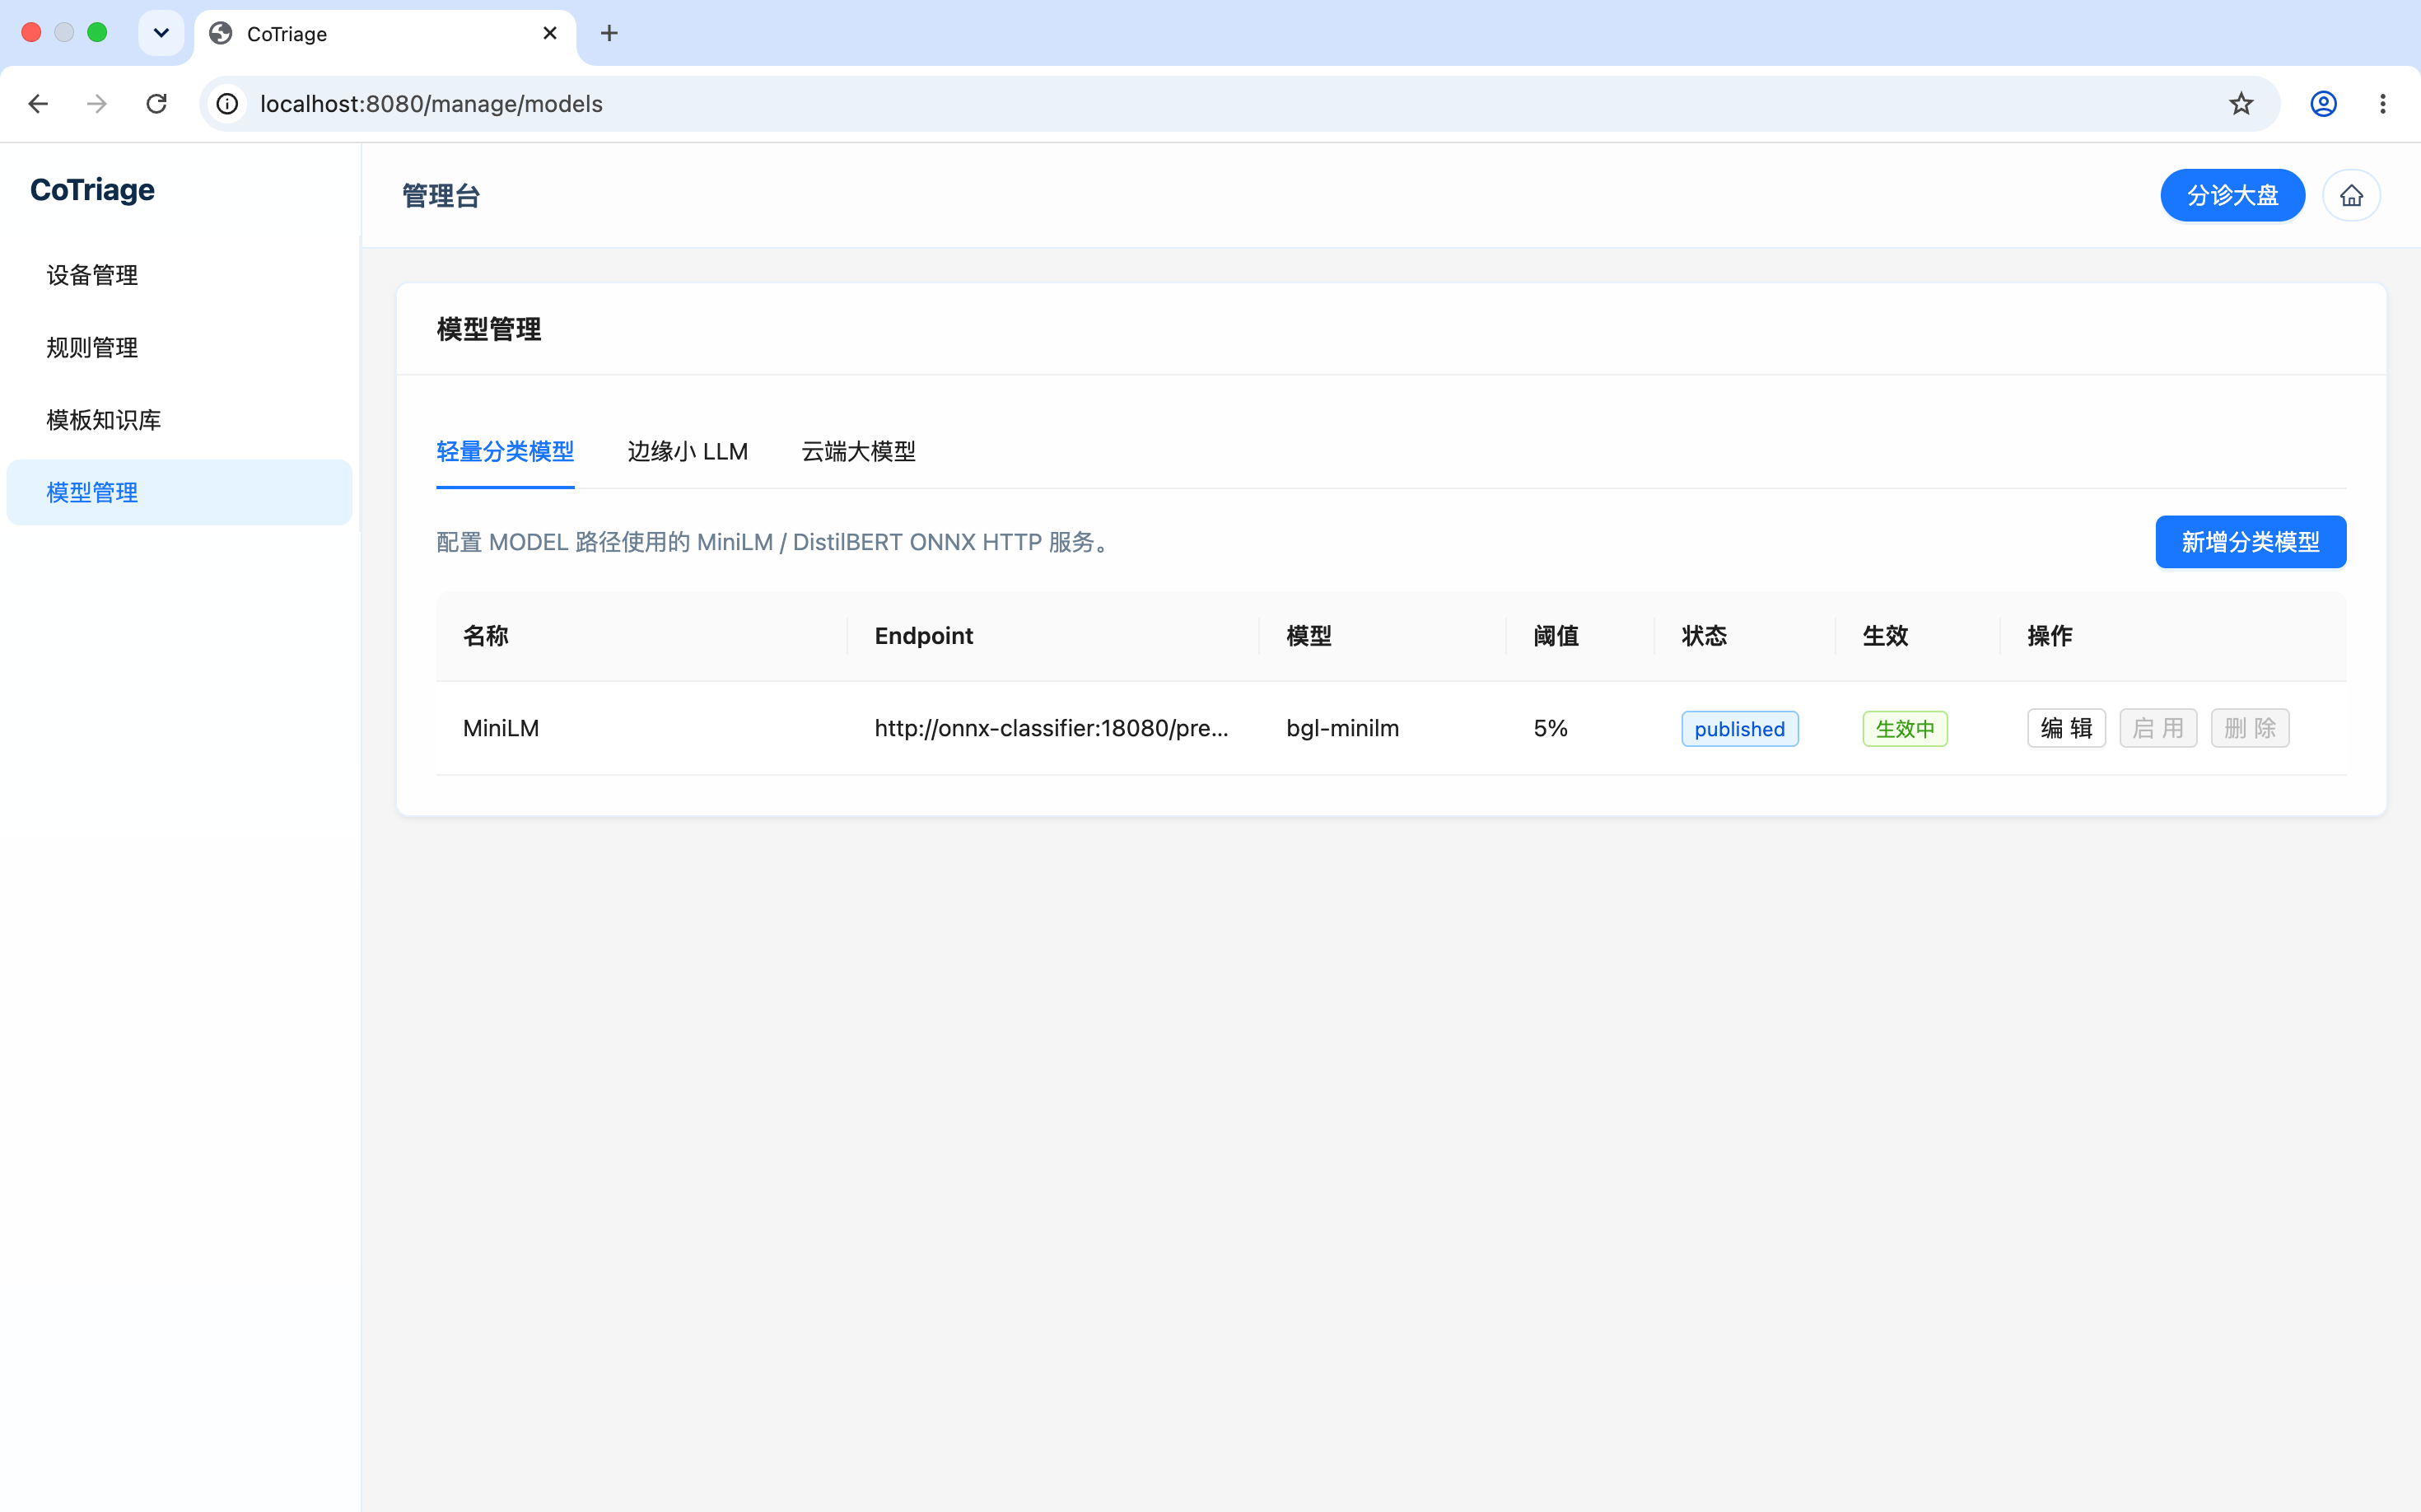
\includegraphics[width=\linewidth]{figures/s-09a-minilm-model-management.png}
    \caption{MiniLM 模型发布与生效}
  \end{subfigure}
  \caption{边缘知识与模型的在线配置入口}
  \label{fig:edge-config}
\end{figure}

\cref{fig:edge-config}说明规则和轻量模型可以通过统一管理台发布并查看生效状态。配置版本与事件结果共同保存，使运维人员能够回答“当时使用了哪一份规则或模型”，也为回滚和问题定位提供基础。

\chapter{RAISE 动态路由与弱网补偿}

边缘推理回答“当前能够看出什么”，RAISE 则回答“下一步应把有限的分析资源用在哪里”。它先评估事件的分析价值，再结合系统当时是否适合调用云端，最终在 \texttt{LOCAL}、\texttt{CLOUD} 和 \texttt{DEFER} 之间选择动作。

\section{联合感知的决策输入}
RAISE（Risk-Aware, uncertainty-calibrated, Intent-constrained, Self-adaptive Edge-cloud routing）不是只看一个置信度阈值。其输入由事件侧和系统侧两组信号构成。

\begin{table}[htbp]
  \centering
  \small
  \caption{RAISE 的联合感知因素}
  \label{tab:raise-inputs}
  \begin{tabularx}{\textwidth}{>{\bfseries}p{0.18\textwidth} p{0.28\textwidth} X}
    \toprule
    信号类别 & 代表因素 & 对决策的影响 \\
    \midrule
    事件风险 & 严重度、影响范围、推理路径风险 & 风险越高，越需要更强诊断与更高处理优先级 \\
    认知不确定性 & 置信度校准、不确定性、模板新颖度、历史边云分歧 & 边缘越没有把握，云端复核价值通常越高 \\
    运行条件 & 网络状态、云端健康、队列压力、调用预算与限流 & 条件恶化时提高即时上云门槛，避免主链拥塞 \\
    运维意图 & 禁止上云、强制本地、强制云端等硬策略 & 明确的隐私与生产规则优先于软评分 \\
    \bottomrule
  \end{tabularx}
\end{table}

事件分数描述“这条事件是否值得获得更强能力”，动态门槛描述“系统此刻能承担多少云端任务”。两者分开后，同一类日志可以在网络畅通与网络受限时得到不同动作，同时保持可解释的原因记录。

\section{价值评分与系统成本建模}
对时刻 $t$ 到达的事件 $e_t$，RAISE 将事件本身的分析价值、云端可能带来的新增收益和当前系统成本组合为
\begin{equation}
  S_t = \beta_v V(e_t) + \beta_g G(e_t) - \beta_k K(e_t,s_t),
  \label{eq:raise-score-v03}
\end{equation}
其中，$V(e_t)$ 由严重度、不确定性、模板新颖度、历史边云分歧、影响范围和推理路径风险构成；$G(e_t)$ 表示云端相对于当前边缘结果可能补充的诊断信息；$K(e_t,s_t)$ 表示调用费用、处理时延、网络压力、队列压力、预算占用和隐私风险等代价。

式\eqref{eq:raise-score-v03}可以直观理解为“事件值得深入分析的程度，加上云端可能带来的认知增益，再减去此刻使用云端的综合代价”。各特征在进入评分前完成归一化，使风险、置信度、字节量和系统压力等不同量纲能够在统一空间中比较。该结构也保留了明确的工程解释：事件侧因素决定是否有必要获得更强能力，状态侧因素决定此时调用这项能力是否划算。

\section{动态门槛与容量调节}
系统门槛定义为
\begin{equation}
  \Theta_t = \Theta_0 + \alpha_q Q_t + \alpha_b B_t + \alpha_n N_t - \alpha_a A_t,
  \label{eq:raise-threshold-v03}
\end{equation}
其中，$Q_t$、$B_t$、$N_t$ 和 $A_t$ 分别表示队列压力、预算压力、网络压力和审计采样不足程度。队列拥塞、预算紧张或网络条件恶化时，门槛随之提高，系统将更多事件保留在边缘或延期处理；近期缺少云端复核样本时，审计项可以适度降低门槛，为边缘结论保留必要的抽样校验。

动态门槛使 RAISE 不必为所有部署环境使用同一个固定置信度阈值。在输入内容相同的情况下，网络畅通、队列空闲且预算充足时，系统可以主动获取更多云端增益；资源紧张时则优先保障现场主链。门槛、压力项和最终动作随事件共同保存，使容量调节不是不可见的内部行为，而是可以被运行界面解释和复盘的决策依据。

\section{三动作在线路由算法}
\begin{algorithm}[htbp]
  \caption{RAISE 三动作在线路由}
  \label{alg:raise-v03}
  \KwInput{事件 $e_t$，边缘结果，系统状态 $s_t$，运维策略}
  \KwOutput{$\texttt{LOCAL}$、$\texttt{CLOUD}$ 或 $\texttt{DEFER}$}
  执行禁止上云、强制本地和强制云端等硬约束\;
  计算事件分数 $S_t$ 与动态门槛 $\Theta_t$\;
  \eIf{$S_t < \Theta_t$}{
    \KwRet{$\texttt{LOCAL}$}\;
  }{
    \eIf{网络、云端健康、预算和限流条件允许}{
      \KwRet{$\texttt{CLOUD}$}\;
    }{
      将事件持久化到优先级 Outbox\;
      \KwRet{$\texttt{DEFER}$}\;
    }
  }
\end{algorithm}

算法\ref{alg:raise-v03}首先执行运维硬约束，再计算软评分。这样的顺序保证禁止上云、数据边界和生产安全策略不会被在线模型或统计分数覆盖。动作产生后，路由器保存事件分数、动态门槛、关键特征、动作原因和系统状态快照，既为管理端提供解释，也为后续策略评估和重放审计提供依据。

\section{反馈信号与自适应衔接}
Cloud Gateway 会依据云端纠正、根因与建议完整性、高风险确认、置信度变化、延迟和 Token 使用构造复合反馈：
\begin{equation}
  r=\operatorname{clip}_{[-1,1]}\!\left(
  0.35D+0.30A+0.20H+0.15\Delta c-0.10L-0.05T
  \right),
  \label{eq:cloud-reward-v03}
\end{equation}
其中，$D$ 表示云端是否有效纠正边缘判断，$A$ 表示是否同时提供根因与建议，$H$ 表示是否确认高风险事件，$\Delta c$ 表示正向置信度变化，$L$ 和 $T$ 分别是归一化后的时延与 Token 惩罚。该反馈把诊断增益和资源成本放入同一信号，为模板纠错统计、探索状态和 GainModel 更新提供输入。

Router 当前会依据首个匹配条件对反馈重新归类，并更新模板统计、探索状态和 GainModel 快照。现有离散归类可能覆盖 Gateway 生成的复合值，已学习增益也尚未直接参与式\eqref{eq:raise-score-v03}。因此，当前反馈链首先承担结果记录、统计更新和后续学习数据积累；进一步自适应需要统一两阶段 Reward 语义，再通过灰度发布、状态快照和可回滚机制安全接入在线评分。

\section{三动作语义}
\begin{table}[htbp]
  \centering
  \small
  \caption{RAISE 三种动作的业务含义}
  \label{tab:raise-actions}
  \begin{tabularx}{\textwidth}{>{\ttfamily\bfseries}p{0.16\textwidth} X X}
    \toprule
    \normalfont\bfseries 动作 & \textbf{触发语义} & \textbf{后续处理} \\
    \midrule
    LOCAL & 边缘已有足够信息，或策略要求留在本地 & 保存并发布边缘判断，供现场系统继续消费 \\
    CLOUD & 事件值得上云，且网络、预算、健康与限流条件允许 & 立即进入云端请求流，聚合上下文后深诊 \\
    DEFER & 事件值得上云，但当前发送条件不满足 & 写入持久化 Outbox，后续按优先级重试 \\
    \bottomrule
  \end{tabularx}
\end{table}

\texttt{DEFER} 的关键意义是把“值得上云”与“现在能够发送”解耦。没有该动作时，断网中的高价值事件只能被迫留在本地或直接失败；引入延期后，实时主链继续产出边缘结果，后续深诊机会则由独立队列保存。

\section{路由运行状态}
\begin{figure}[htbp]
  \centering
  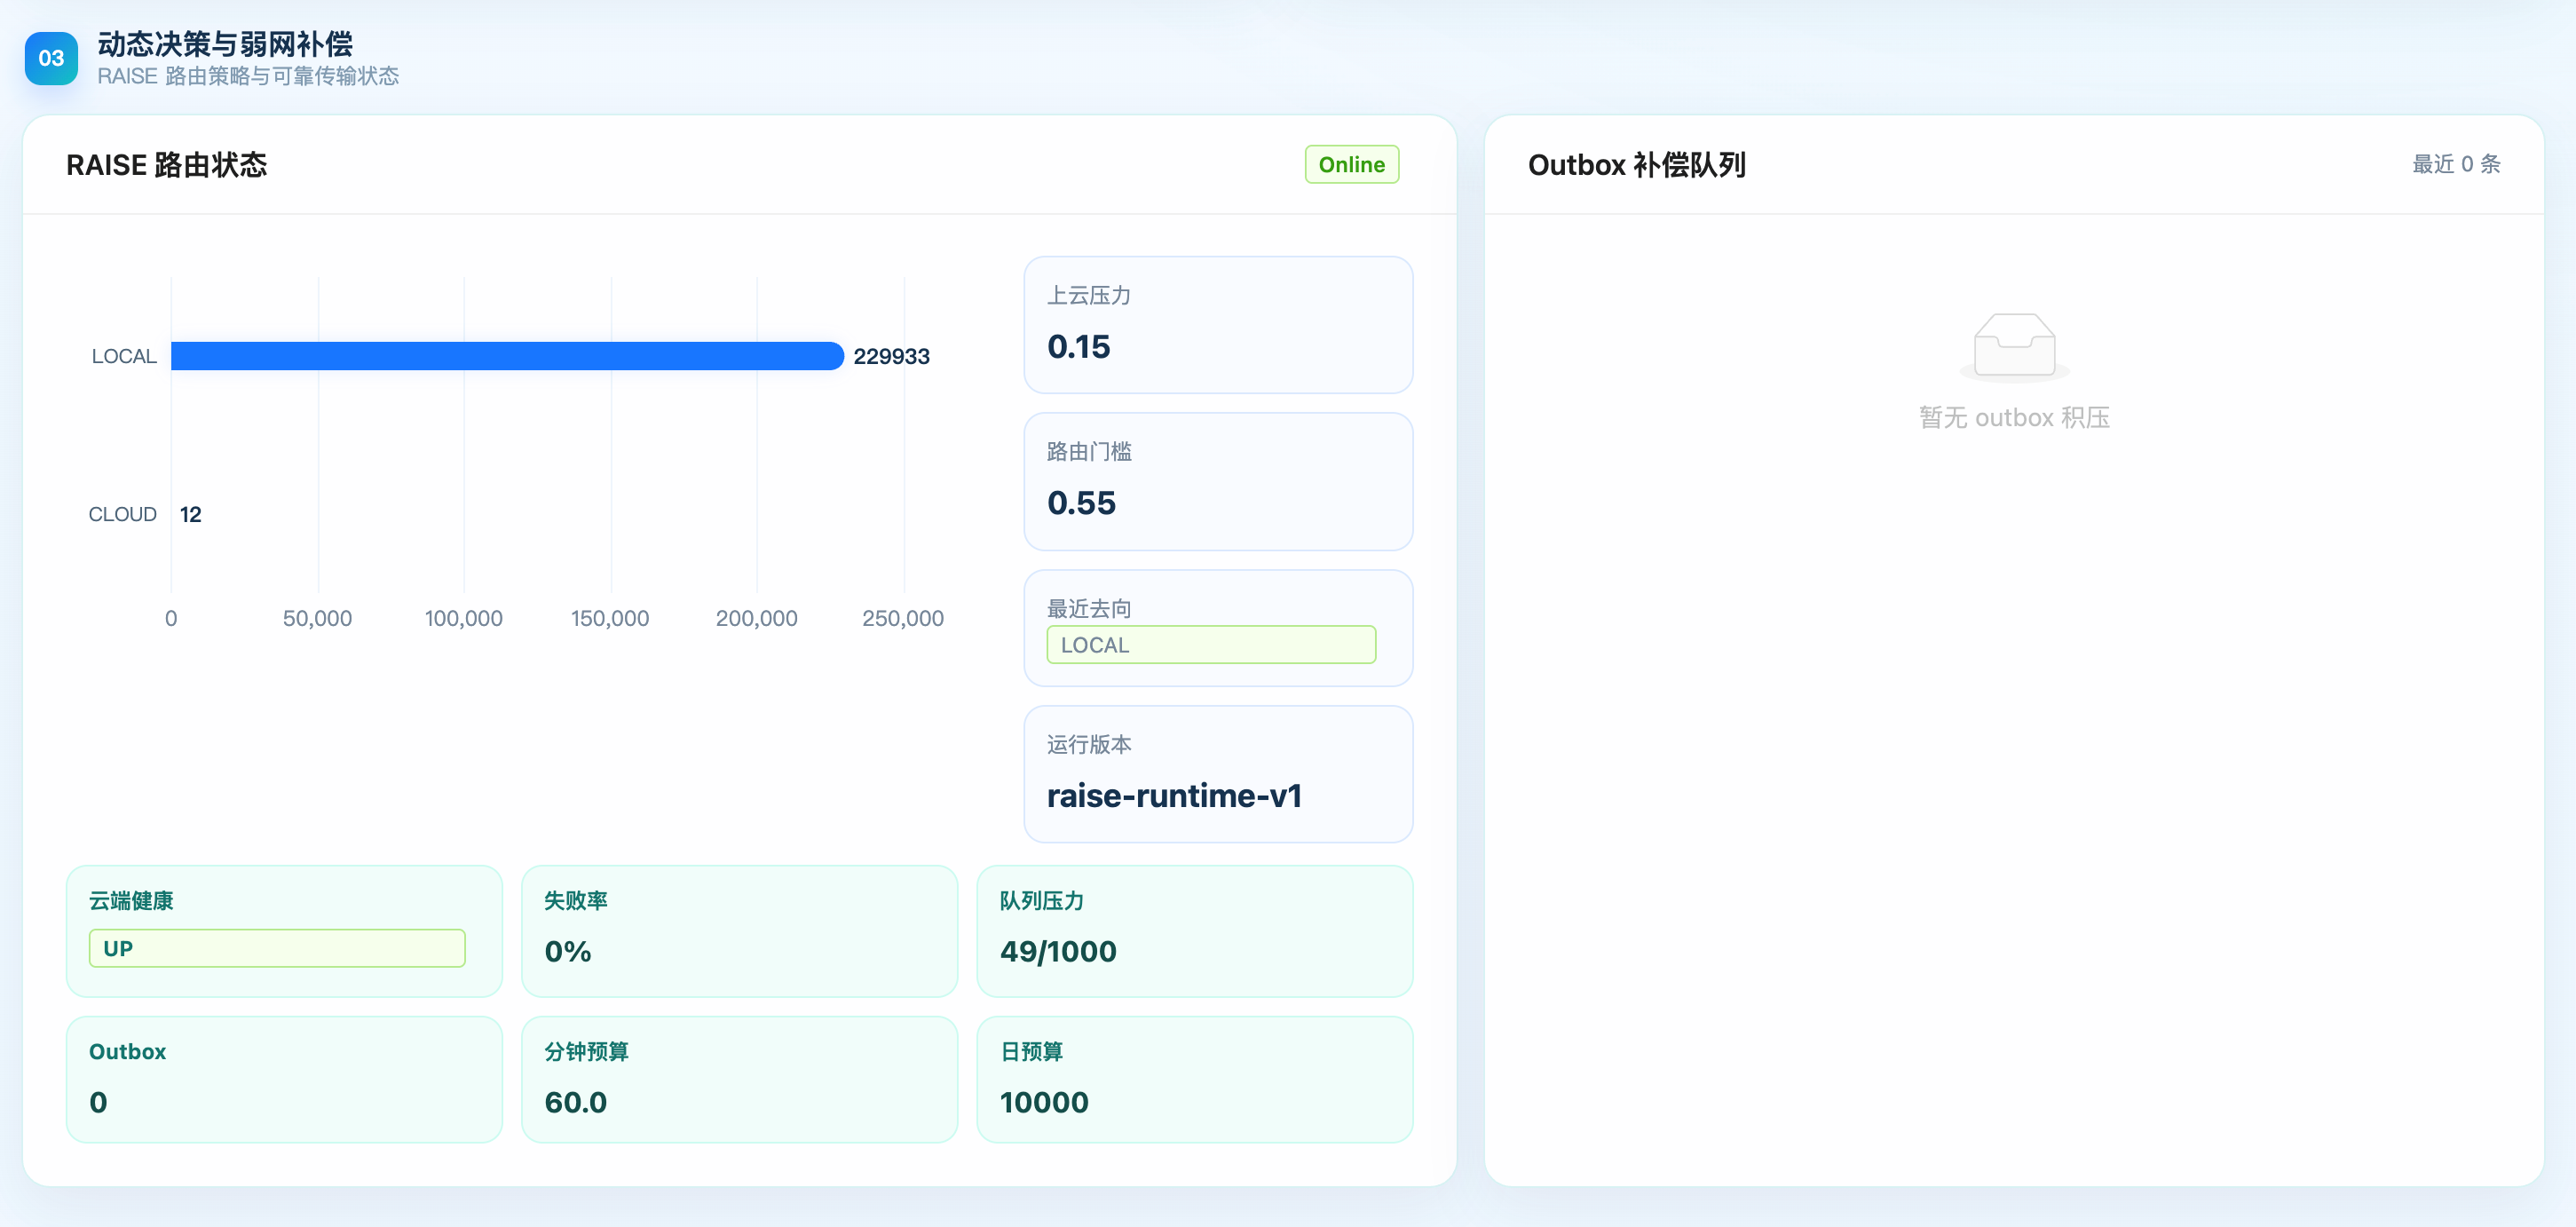
\includegraphics[width=0.98\textwidth]{figures/s-04a-raise-routing-status-overview.png}
  \caption{RAISE 路由状态、系统压力与 Outbox 的统一展示}
  \label{fig:raise-routing-overview}
\end{figure}

\cref{fig:raise-routing-overview}集中展示 \texttt{LOCAL/CLOUD} 累计数量、上云压力、动态门槛、最近动作、云端健康、队列压力、预算与 Outbox。它帮助运维人员判断系统当前如何分流，以及外部条件是否正在改变门槛。该画面是运行窗口的聚合状态；Outbox 为空只说明截图时没有积压，不能据此推断弱网恢复速度或重试成功率。

\section{Outbox 优先补传与死信处理}
当 RAISE 输出 \texttt{DEFER} 时，事件写入 MySQL \texttt{cloud\_outbox}。replayer 周期读取到期记录，多实例通过条件更新抢占任务；失败后按照退避策略重试，超过次数限制的记录进入 DLQ，供运维人员检查。到期任务按照 RAISE 分数降序，再按截止时间与创建时间排序，使更高风险、更紧迫的事件优先获得发送机会。

\begin{figure}[htbp]
  \centering
  \begin{tikzpicture}[
    node distance=11mm and 12mm,
    state/.style={draw=CoTriageNavy,rounded corners=1.2mm,minimum width=24mm,minimum height=10mm,fill=CoTriageGray,font=\sffamily\small\bfseries,text=CoTriageNavy,align=center},
    terminal/.style={state,draw=CoTriageCyan,fill=CoTriageCyan!8},
    failed/.style={state,draw=CoTriageRed,fill=CoTriageRed!7,text=CoTriageRed},
    flow/.style={-{Stealth[length=2.5mm]},thick,draw=CoTriageCyan},
    retry/.style={-{Stealth[length=2.5mm]},thick,dashed,draw=CoTriageOrange}
  ]
    \node[state] (pending) {PENDING\\等待到期};
    \node[state,right=of pending] (sending) {SENDING\\条件抢占};
    \node[terminal,right=of sending] (sent) {SENT\\已发布请求};
    \node[state,below=of sending] (retrying) {RETRY\\退避重试};
    \node[failed,right=of retrying] (dlq) {DLQ\\人工检查};
    \draw[flow] (pending) -- node[above,font=\footnotesize]{按优先级读取} (sending);
    \draw[flow] (sending) -- node[above,font=\footnotesize]{发布成功} (sent);
    \draw[retry] (sending) -- node[right,font=\footnotesize]{失败} (retrying);
    \draw[retry] (retrying.west) -| node[pos=0.25,below,font=\footnotesize]{未超限} (pending.south);
    \draw[retry] (retrying) -- node[above,font=\footnotesize]{超过上限} (dlq);
  \end{tikzpicture}
  \caption{Outbox 延期、重试与死信状态流}
  \label{fig:outbox-state}
\end{figure}

当前实现中的 \texttt{SENT} 表示请求已经发布到云端请求流，并不等同于云端诊断已经完成；replayer 采用周期扫描，也未以网络恢复事件直接触发。这一边界使运行状态的解释更加准确，并为后续增加云端完成确认和健康门控保留了清晰接口。

\section{运维硬策略与可解释性}
禁止上云、强制本地和强制云端等策略先于软评分执行，防止模型覆盖隐私、安全和生产要求。每次路由同时保留动作、原因、分数、门槛与系统快照，使管理员既能查看“去了哪里”，也能追溯“当时为什么这样决定”。

\chapter{云端根因诊断与反馈闭环}

\section{从单事件到关联上下文}
边缘推理擅长在低时延条件下处理单条或局部事件，云端诊断的价值则来自更强的语义能力与更完整的上下文。\texttt{cloud-gateway} 围绕主事件，从近期边缘事件中按照时间、模板、来源、设备、类别和严重度选择相关记录，并在 Token 预算内裁剪。它不是无边界地拼接全部日志，而是组织一份与当前问题直接相关的诊断材料。

时间邻近可以提示故障传播顺序，相同设备或模板可以提示重复模式，跨来源的高严重度事件则可能指向共同依赖故障。上云前，系统对主事件和关联事件的原始日志执行常见敏感模式脱敏；进一步工程化还需将模板、设备、来源和其他提示字段纳入统一字段级策略。

\section{异常态势与云端深诊}
\begin{figure}[htbp]
  \centering
  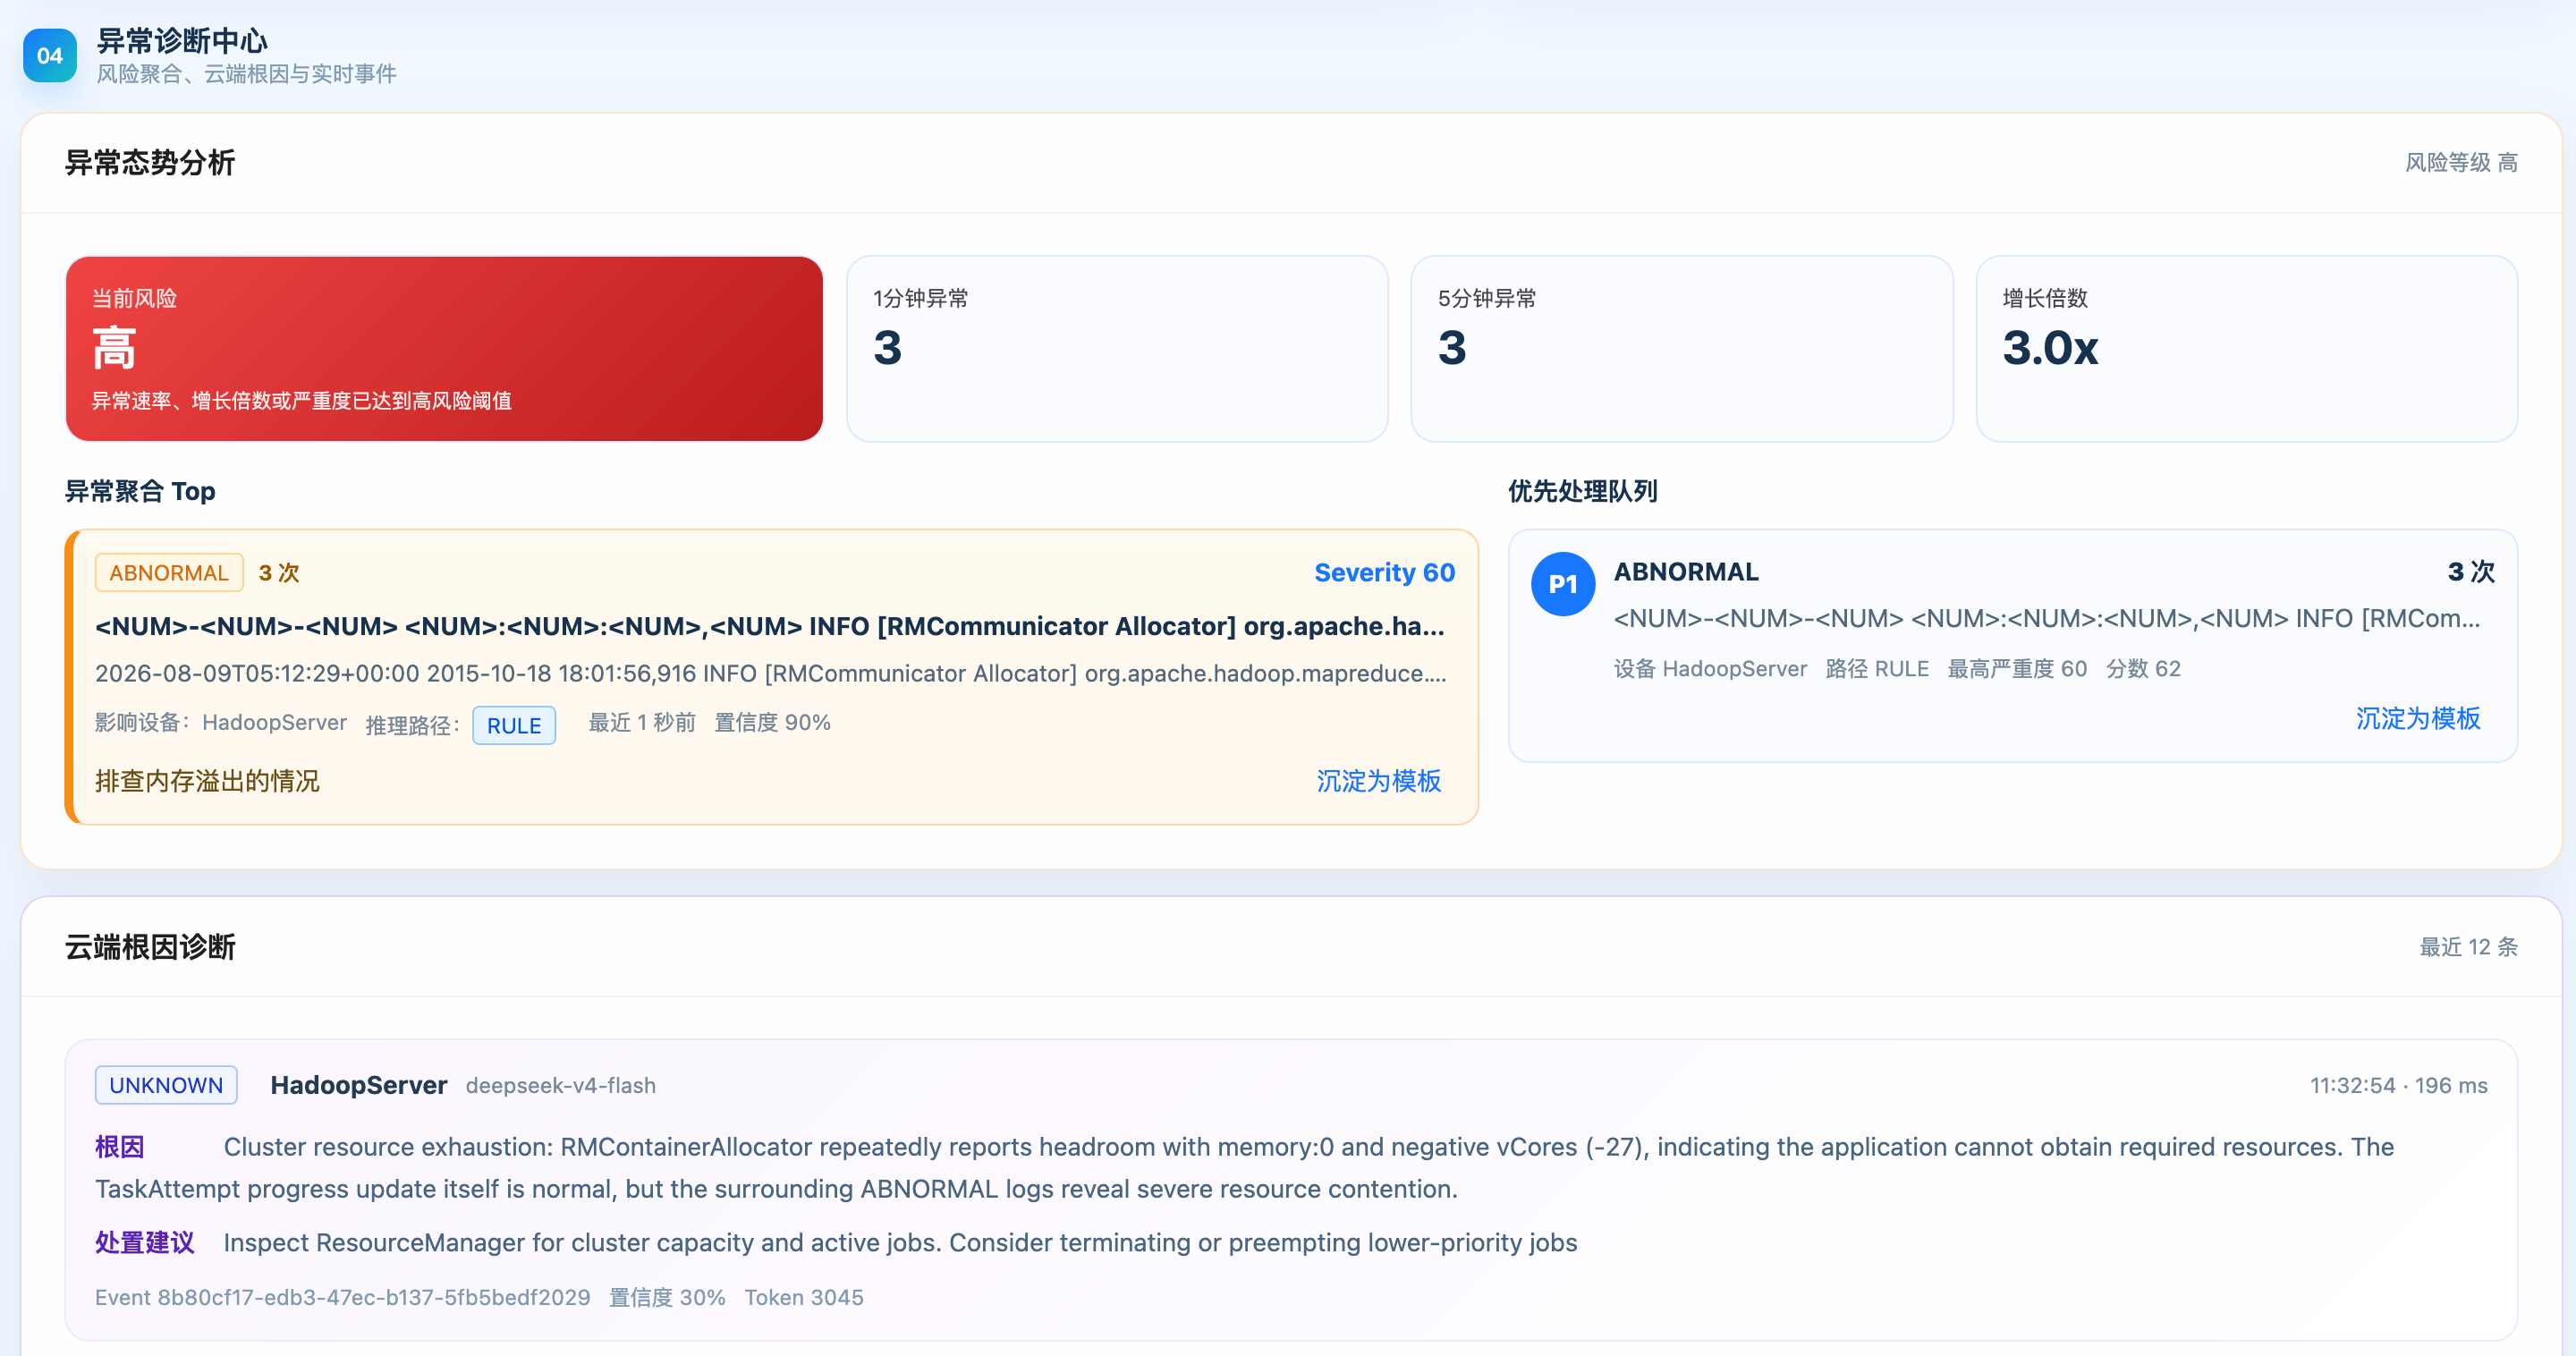
\includegraphics[width=0.98\textwidth]{figures/s-03b-anomaly-diagnosis-center-overview.png}
  \caption{异常态势、优先队列与云端根因诊断的统一界面}
  \label{fig:diagnosis-center}
\end{figure}

\cref{fig:diagnosis-center}把异常趋势、风险聚合、优先处理队列、云端根因诊断和实时事件放在同一页面中。运维人员可以先从总体风险发现问题，再沿具体事件下钻到诊断结果。页面中边缘字段与云端字段属于不同处理阶段，不应仅凭标签差异计算判断准确率或冲突解决效果。

\begin{figure}[htbp]
  \centering
  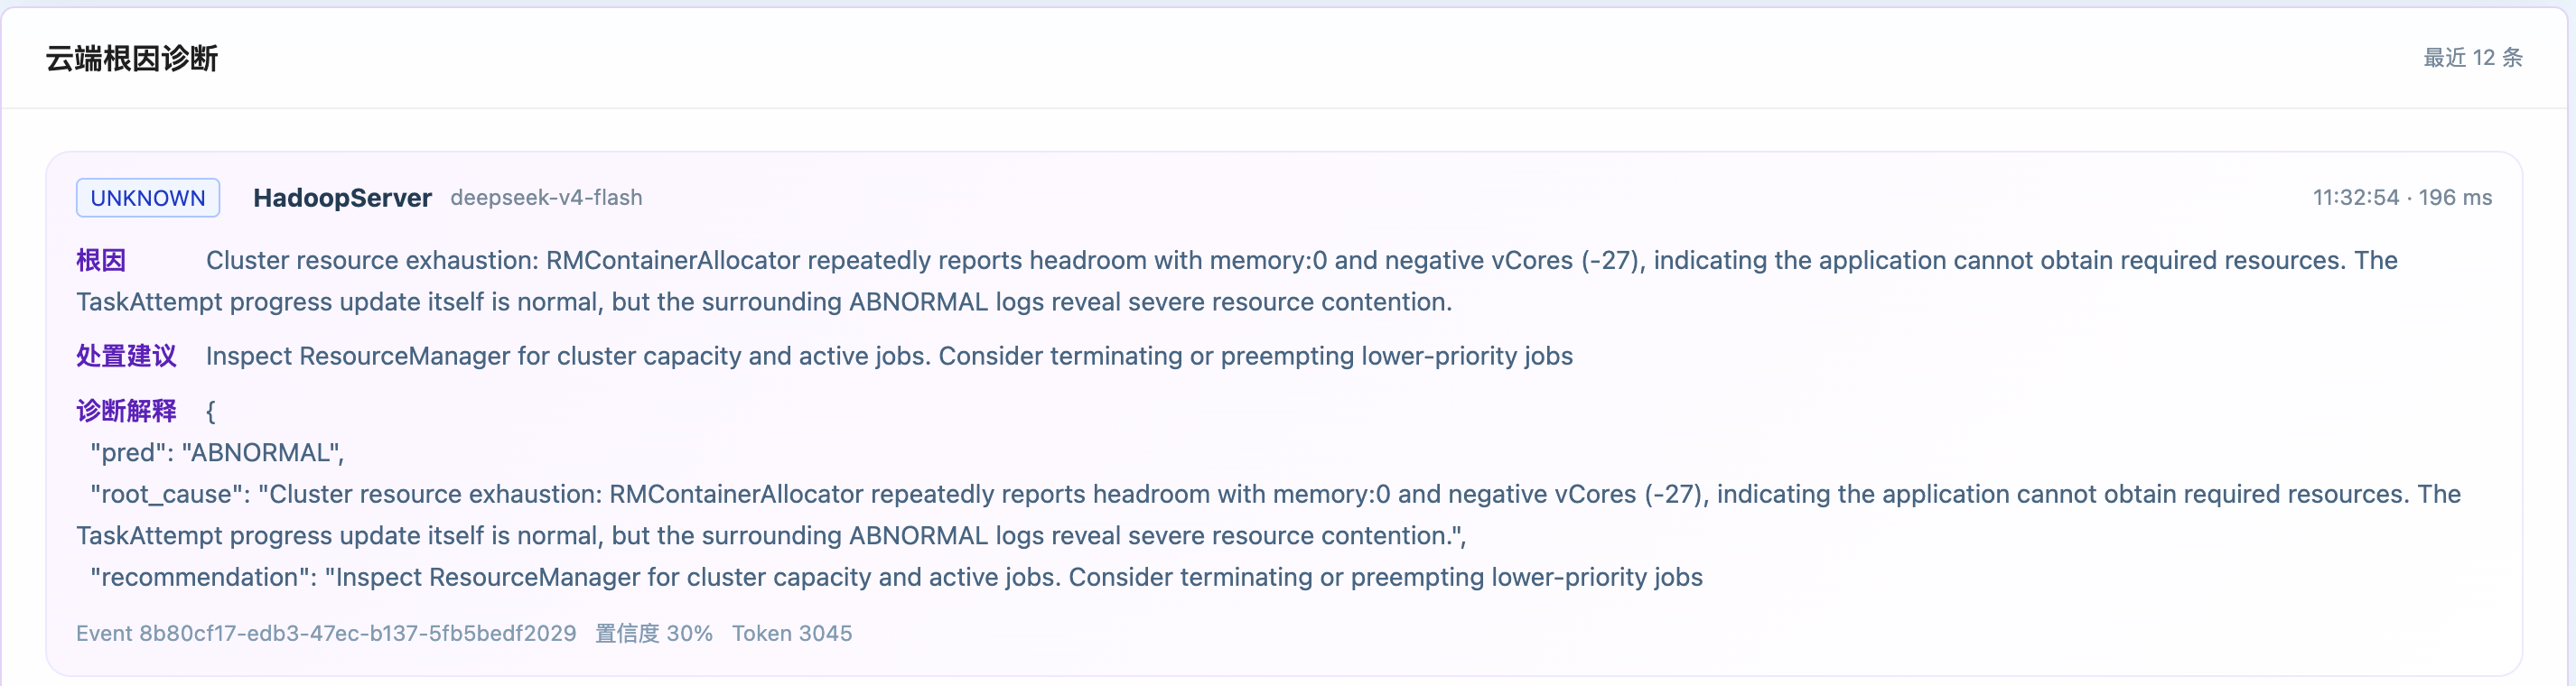
\includegraphics[width=0.98\textwidth]{figures/s-05a-cloud-root-cause-diagnosis.png}
  \caption{云端结构化根因、处置建议与诊断解释}
  \label{fig:cloud-root-cause-diagnosis-v03}
\end{figure}

\cref{fig:cloud-root-cause-diagnosis-v03}展示了单条云端诊断的详细形态。系统不仅呈现一个类别，还同时保留模型信息、根因候选、处置建议、结构化解释、置信度、Token 用量与处理时延，使“发生了什么”“为什么这样判断”“下一步可以做什么”能够在同一结果中被阅读。

\section{结构化输出与降级解析}
云端模型的理想输出是稳定 JSON，但真实 Provider 可能返回被代码块包裹的 JSON、夹杂说明文本的对象，甚至完全非结构化的内容。网关因此采用分级解析：优先严格解析完整对象，其次提取文本中的对象片段，仍无法解析时保留原文并进入明确降级路径。主要字段如\cref{tab:cloud-output}所示。

\begin{table}[htbp]
  \centering
  \small
  \caption{云端诊断输出及其运维用途}
  \label{tab:cloud-output}
  \begin{tabularx}{\textwidth}{>{\ttfamily}p{0.22\textwidth} X X}
    \toprule
    \normalfont\bfseries 字段 & \textbf{含义} & \textbf{界面用途} \\
    \midrule
    pred / confidence & 云端复判类别及把握程度 & 与边缘初判并列查看 \\
    root\_cause & 结合关联上下文形成的根因候选 & 支持故障定位与影响分析 \\
    recommendation & 面向运维人员的处置建议 & 连接诊断与后续行动 \\
    explanation & 结构化诊断依据或原始解析内容 & 支持审阅、追踪与降级展示 \\
    latency / token & 本次调用时延与 Token 用量 & 进入运行成本和性能观测 \\
    \bottomrule
  \end{tabularx}
\end{table}

\section{幂等写回与在线反馈}
云端结果先依据幂等键写入 MySQL，再发布响应通知，最后确认请求消息。如果持久化已经完成而通知失败，重试可以复用既有结果，避免再次调用云端模型。该顺序把高成本调用置于幂等边界内，降低重复计费和结果漂移风险。

反馈处理会根据云端是否纠正边缘判断、是否补充根因与建议、是否确认高风险事件等信号更新模板统计、探索状态和 GainModel 快照。当前已学习增益尚未直接进入 RAISE 决策分数，两阶段 Reward 的语义也需要进一步统一。因此，现阶段更准确的定位是“具有结构化反馈和在线统计的动态路由”，而不是已经由反馈完全自适应的闭环。反馈公式及其与在线评分的衔接方式见第 6 章。

\section{从诊断到业务处置}
核心仓库将结构化结果保存并开放给查询与展示接口，不内置生产现场的自动处置执行器。实际落地时，可由告警平台、工单系统或设备控制系统订阅本地和云端结果，并根据自身权限与安全策略执行后续动作。这样既避免诊断系统越权控制生产设备，也为不同企业的处置流程保留接入空间。

\chapter{工程实现}

\section{工程组织与组件边界}
CoTriage 采用面向事件流的多进程实现，而不是将采集、推理、路由和云端调用堆叠在一个服务中。工程主体由 Go、Python 和 Vue 组成：Go 负责长时间运行的采集、消息消费、路由、云端网关和控制接口；Python 以独立 HTTP 服务封装 MiniLM ONNX Runtime；Vue 3 管理端负责运行观测与配置操作。Redis Streams 连接实时处理链，MySQL 保存需要跨重启保留的决策、Outbox、反馈和配置状态。各组件只通过版本化事件、Stream 或 HTTP 契约协作，不共享进程内对象，因此能够分别扩展、替换和故障隔离。

\begin{table}[htbp]
  \centering
  \small
  \caption{主要工程组件、输入输出与持久状态}
  \label{tab:implementation-components}
  \begin{tabularx}{\textwidth}{>{\ttfamily}p{0.18\textwidth} p{0.25\textwidth} p{0.26\textwidth} X}
    \toprule
    \normalfont\bfseries 组件 & \textbf{主要输入} & \textbf{主要输出} & \textbf{状态与部署} \\
    \midrule
    log-collector & 节点日志文件、Node 元数据 & \texttt{events.raw} & 无中心状态；DaemonSet 逐节点部署 \\
    edge-infer & \texttt{events.raw}、边缘配置 & \texttt{events.inferred}、DLQ & 模板缓存、幂等键；Deployment \\
    onnx-classifier & 标准化模板文本 & 二分类概率与模型版本 & ONNX 模型常驻内存；Deployment \\
    \makecell[l]{router-\\controller} & \texttt{events.inferred}、运行状态 & \texttt{events.routed}、云请求、Outbox & 决策、快照、反馈；Deployment \\
    cloud-gateway & 云请求、关联事件、Provider 配置 & \texttt{events.cloud.resp}、反馈记录 & 幂等结果与调用用量；Deployment \\
    server & Redis、MySQL、Kubernetes API & REST、SSE、配置接口 & 配置与查询控制面；Deployment \\
    web & REST 历史快照、SSE 增量事件 & 驾驶舱与管理操作 & 浏览器状态；Nginx Deployment \\
    \bottomrule
  \end{tabularx}
\end{table}

每个 Go 组件均拥有独立的 \texttt{go.mod}、进程入口、配置包和 Dockerfile，模型服务与 Web 同样独立构建镜像。这样的仓库组织与运行边界保持一致：采集器升级不会要求重新打包路由器，云端 Provider 变更也不会影响边缘推理进程。事件中的 \texttt{schema\_version}、模型版本、规则版本和路由版本共同构成运行时坐标，使一次结果能够定位到产生它的代码路径和配置状态。

\section{采集与消息传输实现}
\subsection{节点就近采集}
\texttt{log-collector} 以 DaemonSet 运行在每个接入节点，通过 Downward API 获得 \texttt{NODE\_NAME}，再使用 Kubernetes 客户端读取节点标签 \texttt{cotriage.io/equipment}。标签读取失败时回退到环境变量或主机名，从而保证事件始终具有设备标识。采集器等待目标日志文件出现，从文件末尾持续读取新增行，为每行生成 UUID 和 UTC 纳秒时间戳，并将原始内容封装为统一事件写入 \texttt{cotriage.events.raw}。Stream 写入使用近似 \texttt{MAXLEN} 控制长度，Redis 短时失败时执行退避而不是形成高频重试循环。

\subsection{Stream 拓扑与消费语义}
实时主链使用五条 Redis Stream 分隔处理阶段，避免慢组件阻塞上游：

\begin{table}[htbp]
  \centering
  \small
  \caption{核心 Redis Streams 及其生产消费关系}
  \label{tab:stream-topology-implementation}
  \begin{tabularx}{\textwidth}{>{\ttfamily}p{0.26\textwidth} p{0.23\textwidth} p{0.23\textwidth} X}
    \toprule
    \normalfont\bfseries Stream & \textbf{生产者} & \textbf{消费者} & \textbf{承载内容} \\
    \midrule
    \makecell[l]{cotriage.events.\\raw} & log-collector & edge-infer & 原始统一事件 \\
    \makecell[l]{cotriage.events.\\inferred} & edge-infer & router-controller & 边缘判断、证据与分阶段耗时 \\
    \makecell[l]{cotriage.events.\\routed} & router-controller & server & 动作、分数、门槛与运行快照 \\
    \makecell[l]{cotriage.events.\\cloud.req} & router & cloud-gateway & 裁剪后的上云请求与幂等字段 \\
    \makecell[l]{cotriage.events.\\cloud.resp} & cloud-gateway & server／反馈链 & 结构化诊断、用量和反馈 \\
    \makecell[l]{cotriage.events.\\dlq} & 各处理组件 & 运维与管理端 & 超限消息、原始字段和错误原因 \\
    \bottomrule
  \end{tabularx}
\end{table}

边缘推理、路由和云端网关使用 Consumer Group 读取新消息，并在下游发布或持久化成功后才确认原消息。边缘推理通过 \texttt{XAUTOCLAIM} 接管空闲时间超过阈值的 Pending 消息，处理失败次数保存在带 TTL 的 Redis Hash 中；超过最大次数后，组件将来源 Stream、消息 ID、消费者组、尝试次数、错误和原始字段一并写入 DLQ，再确认原消息。成功事件以 \texttt{event\_id} 对应的 24 小时幂等键去重，避免 Pending 接管或重试重复产生下游结果。组件还周期裁剪 raw、inferred 和 DLQ，防止持续回放使 Redis 无限增长。

\section{边缘分层推理的代码实现}
\texttt{edge-infer} 将推理能力封装在可热切换的 \texttt{Engine} 中。一次处理首先限制日志最大字节数并执行规范化，生成稳定模板文本和模板 ID；随后依次调用规则引擎、静态或 Redis 模板缓存、HTTP 轻量分类器和可选边缘小语言模型。每一层都返回统一的预测、严重度、置信度、证据、建议和版本字段，因此上游无需了解结果来自规则、缓存还是模型。

规则路径按优先级匹配正则、包含关系或关键词组合，命中明确知识后提前结束，并把高置信模板以 TTL 写入 Redis。模板路径先查进程内发布配置，再查带规则版本的 Redis 缓存；缓存异常只附加到 \texttt{evidence}，不会阻断主结果。模型路径通过带超时的 HTTP 客户端调用 MiniLM ONNX 服务，将 \texttt{NON\_ALERT/ALERT} 映射为统一的 \texttt{NORMAL/ABNORMAL}。当结果为异常且已配置边缘 LLM 时，再调用 OpenAI-compatible 接口生成 \texttt{APP\_ERROR}、\texttt{NET\_ERROR}、\texttt{DISK\_ERROR} 等细分类。模型不可用时返回显式 \texttt{FALLBACK/UNKNOWN}，而不是让消息永久停留在 Pending。

Engine 分别记录规范化、缓存、轻量模型和边缘 LLM 的阶段耗时，并在结果完成时记录总耗时。知识与模型对象由读写锁保护：事件处理时取得只读快照，远程配置线程则在新配置完整解析和校验成功后一次性替换规则、模板、分类器和小模型客户端。配置同步请求携带 \texttt{If-None-Match}，服务端返回 304 时不重复构造对象；拉取、解析或校验失败时继续使用上一份有效配置，避免半份配置进入实时主链。

\section{路由控制器与可靠状态实现}
\texttt{router-controller} 启动时连接 MySQL 与 Redis，可通过 GORM AutoMigrate 初始化表结构，并从最新 \texttt{router\_state\_snapshots} 恢复历史窗口、模板统计和 GainModel 状态。主 Worker 消费边缘结果，运行态构造器同时读取云请求队列、Consumer Group Pending、Outbox 积压以及预算和健康状态，再交给 RAISE 计算动作。路由结果发布到 \texttt{events.routed}，同时以 \texttt{event\_id} 唯一索引写入 \texttt{router\_decisions}，保存边缘结果、动作原因、分数、门槛、策略引用、模型与规则版本以及路由耗时。

对于 \texttt{CLOUD}，Worker 生成 \texttt{request\_id} 和 \texttt{idempotency\_key} 并发布云请求；对于 \texttt{DEFER}，同样的请求正文与路由快照写入 \texttt{cloud\_outbox}。Outbox 记录包含优先分数、截止时间、重试次数、下一次执行时间、锁持有者和最近错误。replayer 每个周期先把锁超时的 \texttt{SENDING} 记录恢复为可重试状态，再按批次查询到期任务；多个实例通过条件更新竞争锁，只有抢占成功的实例可以发布。失败任务采用指数退避，最长退避一分钟，超过最大尝试次数后转入 \texttt{DLQ}。这种数据库条件锁避免了多副本同时补发同一请求。

路由进程还独立运行反馈处理器。云端反馈以 \texttt{event\_id} 唯一保存，处理器批量读取尚未消费的记录，更新模板纠错统计、探索窗口和 GainModel 快照，并标记处理完成。主 Worker、replayer 与反馈处理器共享持久层但运行在独立 goroutine 中，使实时路由、弱网恢复和学习统计不会相互串行阻塞。

\section{云端上下文诊断实现}
\texttt{cloud-gateway} 使用 Consumer Group 批量读取 \texttt{events.cloud.req}，并用容量受限的 semaphore 控制并发 goroutine 数量，避免 Provider 变慢时无限创建请求。消息解码阶段同时校验 Stream 字段、请求正文和 \texttt{event\_id} 一致性；处理前查询反馈表，如果该事件已经完成，则直接重新发布已保存的响应并确认消息，从而使重放过程保持幂等。

上下文聚合器以主事件时间为中心，从 inferred Stream 读取候选事件，并按照时间邻近、模板一致、来源一致、设备一致、预测一致和严重度计算相关分数。候选项排序后受最大事件数和近似 Token 字节预算双重裁剪，再生成 Top 模板、Top 来源、Top 预测、最高严重度和时间跨度等摘要。这样，云端模型获得的是围绕主事件筛选出的证据集合，而不是无边界拼接历史日志。

在构造提示词前，网关对主事件和关联事件中的 IPv4、邮箱、口令、Token、API Key、Secret 和长哈希执行模式化替换，并再次限制原文字符数。Provider 客户端采用 OpenAI-compatible 协议，活动 Provider 由 Server 控制面提供；网关启动时加载一次并周期刷新，数据库只保存密钥对应的环境变量名，不在接口中返回明文密钥。模型响应必须解析为受约束的 JSON 结构，随后生成根因、建议、解释、置信度、Token、时延和成本字段。可重试的超时、限流和 5xx 错误保留在 Pending 等待后续处理，不可重试的配置或格式错误写入响应流与 DLQ。

\section{控制面与数据查询实现}
\texttt{server} 基于 Gin 提供 REST 与 SSE 接口，内部按 \texttt{handler/store/model} 分层：Handler 负责参数和 HTTP 语义，Store 封装 Redis/MySQL 查询，Model 固定对外字段。服务聚合 Kubernetes、Redis 和 MySQL 三类状态：设备接口使用集群内 ServiceAccount 查询 Node 及标签；驾驶舱接口读取近期 inferred 事件并计算趋势、异常比例和推理路径；路由接口查询决策、状态快照、Outbox 和云端反馈；配置接口管理规则、模板、分类器、边缘 LLM 和云端 Provider。

配置对象采用草稿、发布、生效和软删除状态。激活配置时递增 \texttt{config\_version} 并生成 ETag，边缘配置接口支持 \texttt{If-None-Match}；活动配置不能直接删除，避免运行组件指向不存在的版本。对尚未初始化的路由表，查询接口采用降级安全策略返回空集合而不是使整个 Server 崩溃，使组件能够按依赖顺序逐步启动。

\begin{figure}[htbp]
  \centering
  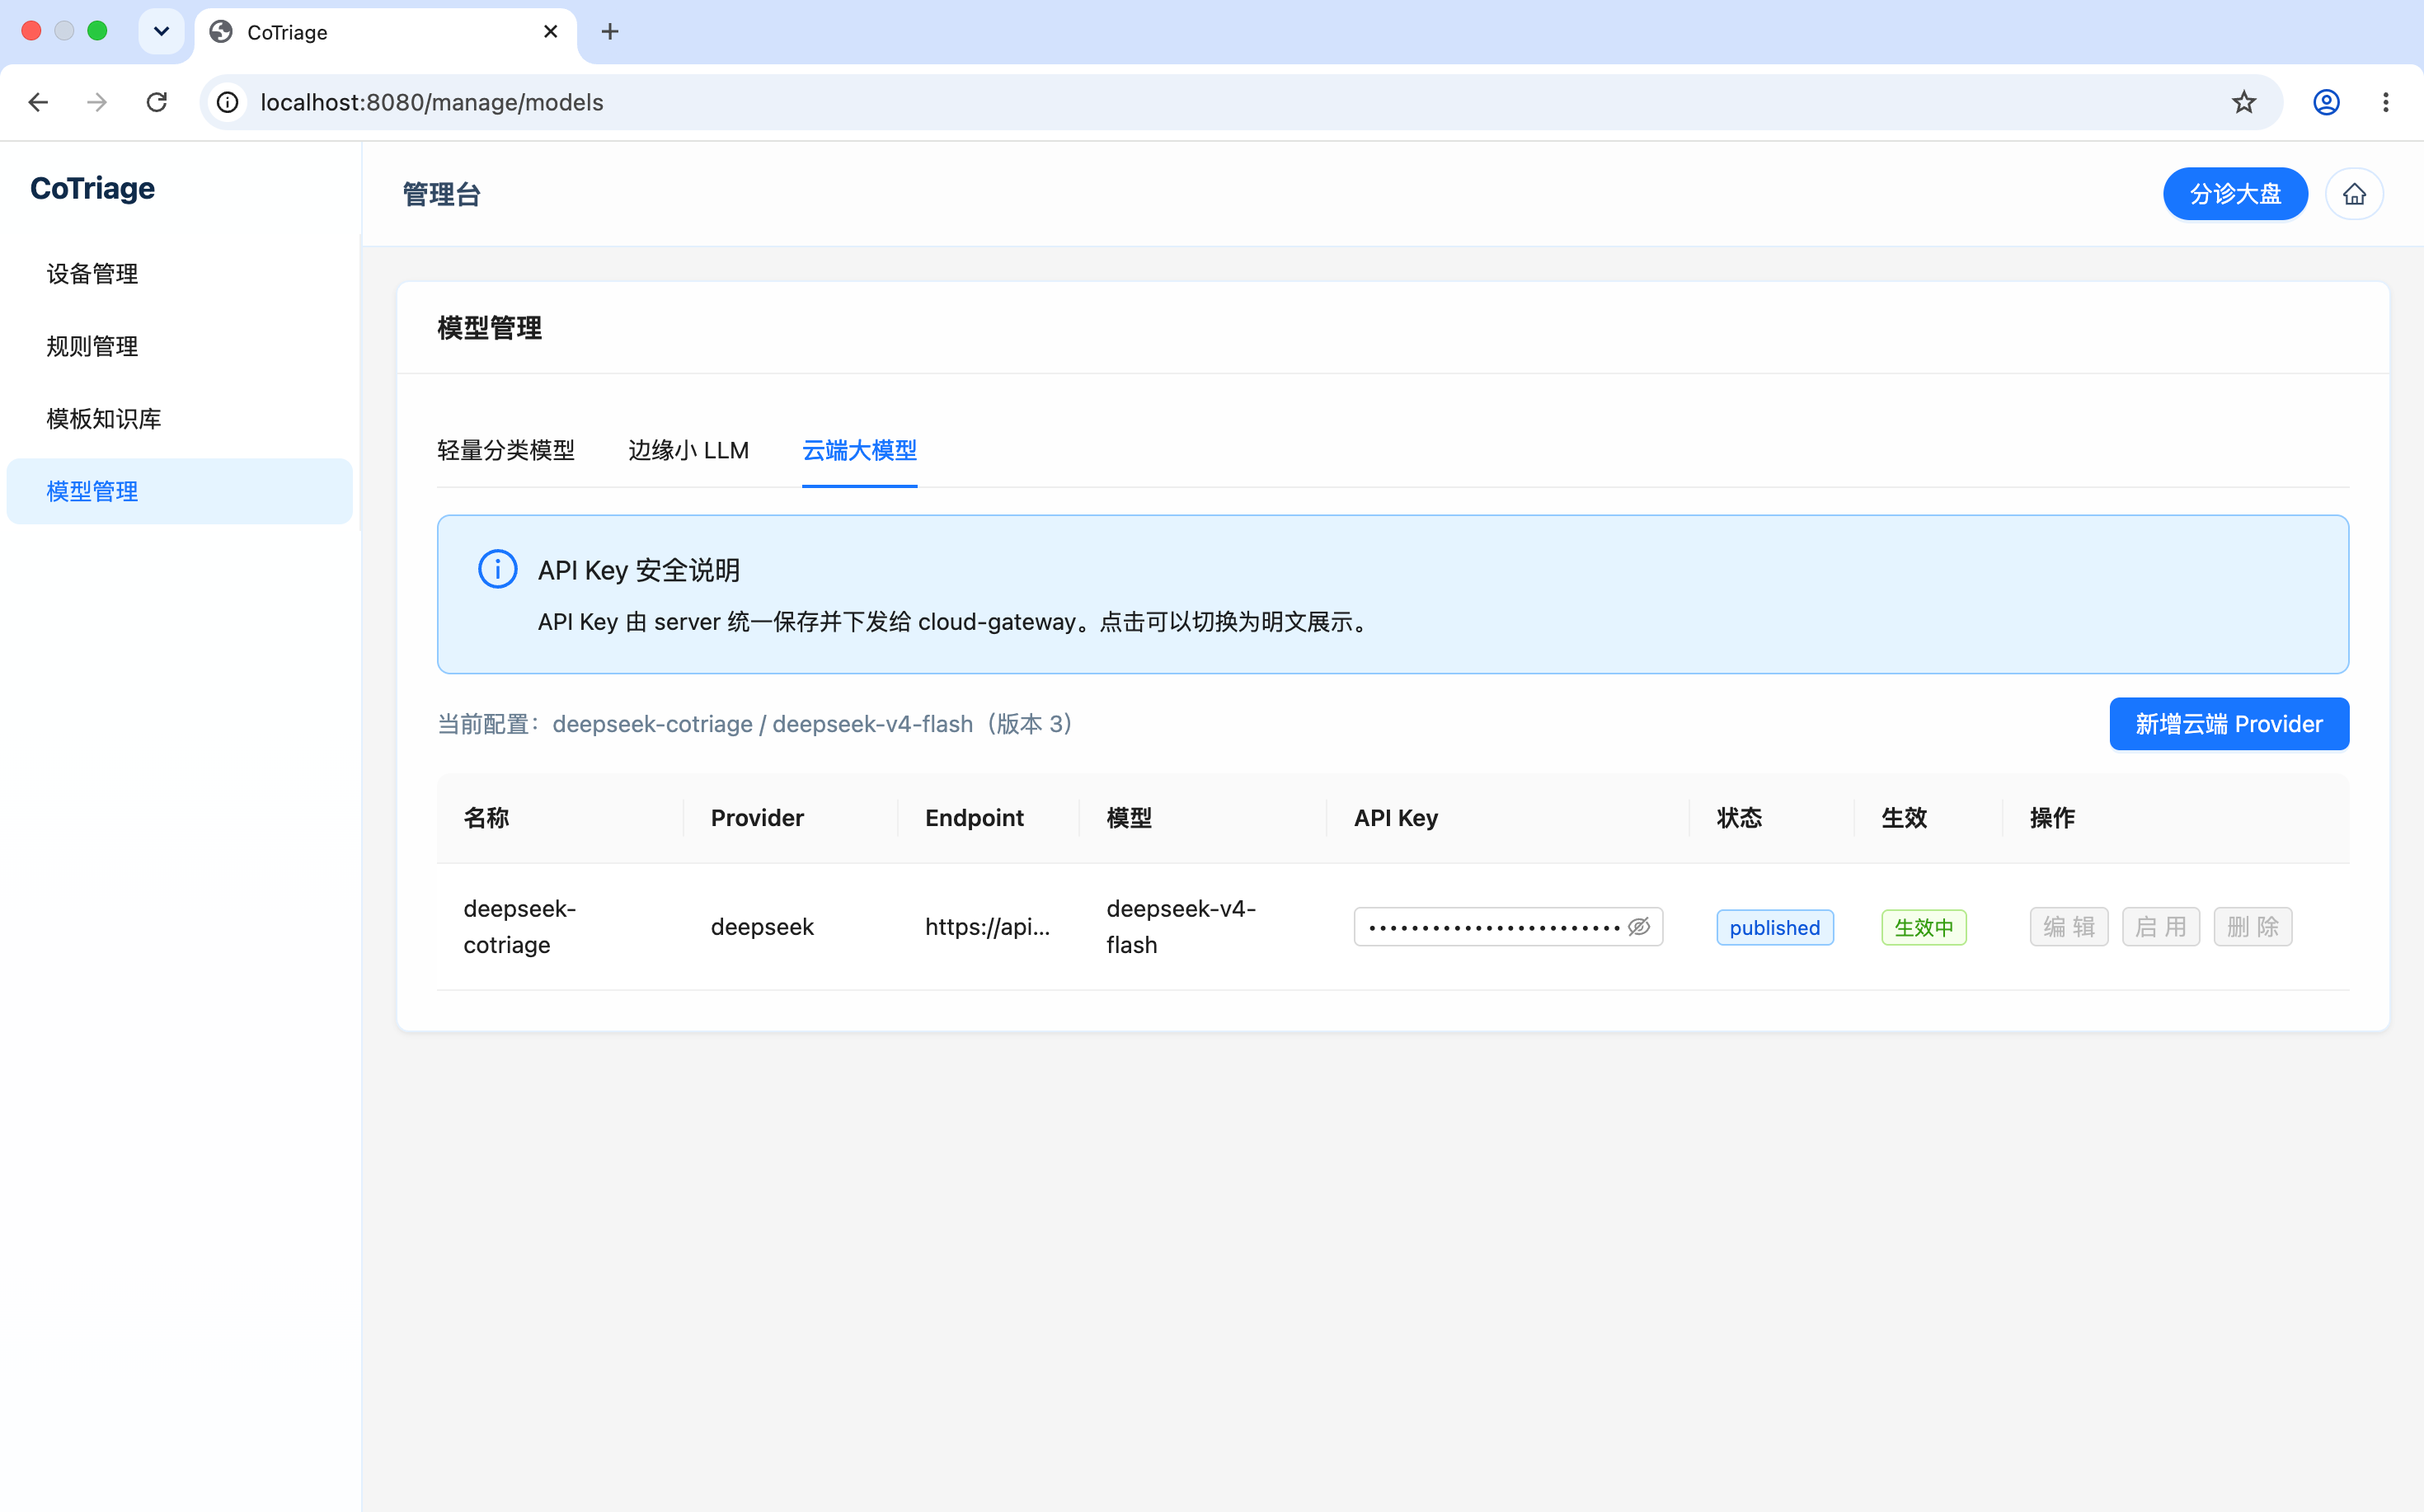
\includegraphics[width=0.96\textwidth]{figures/s-09c-cloud-provider-management.png}
  \caption{云端 Provider、模型参数、发布状态与密钥遮罩管理}
  \label{fig:cloud-provider-management}
\end{figure}

\cref{fig:cloud-provider-management}对应控制面的云模型配置实现。前端提交 Provider 名称、兼容接口地址、模型、超时、最大 Token 与密钥环境变量名；Server 校验后保存版本，Cloud Gateway 只读取当前活动且已发布的配置。

\section{Web 驾驶舱与实时交互实现}
\begin{figure}[htbp]
  \centering
  
\includegraphics[width=0.98\textwidth]{figures/s-00-application-homepage.png}
  \caption{CoTriage 应用首页与核心能力入口}
  \label{fig:application-homepage}
\end{figure}

Web 使用 Vue 3、TypeScript、Vue Router、Ant Design Vue 和 ECharts 实现，由 Nginx 提供静态资源并将 \texttt{/api} 代理到 Server。\cref{fig:application-homepage}不是独立宣传页，而是产品导航入口：实时驾驶舱面向值守和演示，管理中心面向设备、知识和模型治理。

\begin{figure}[htbp]
  \centering
  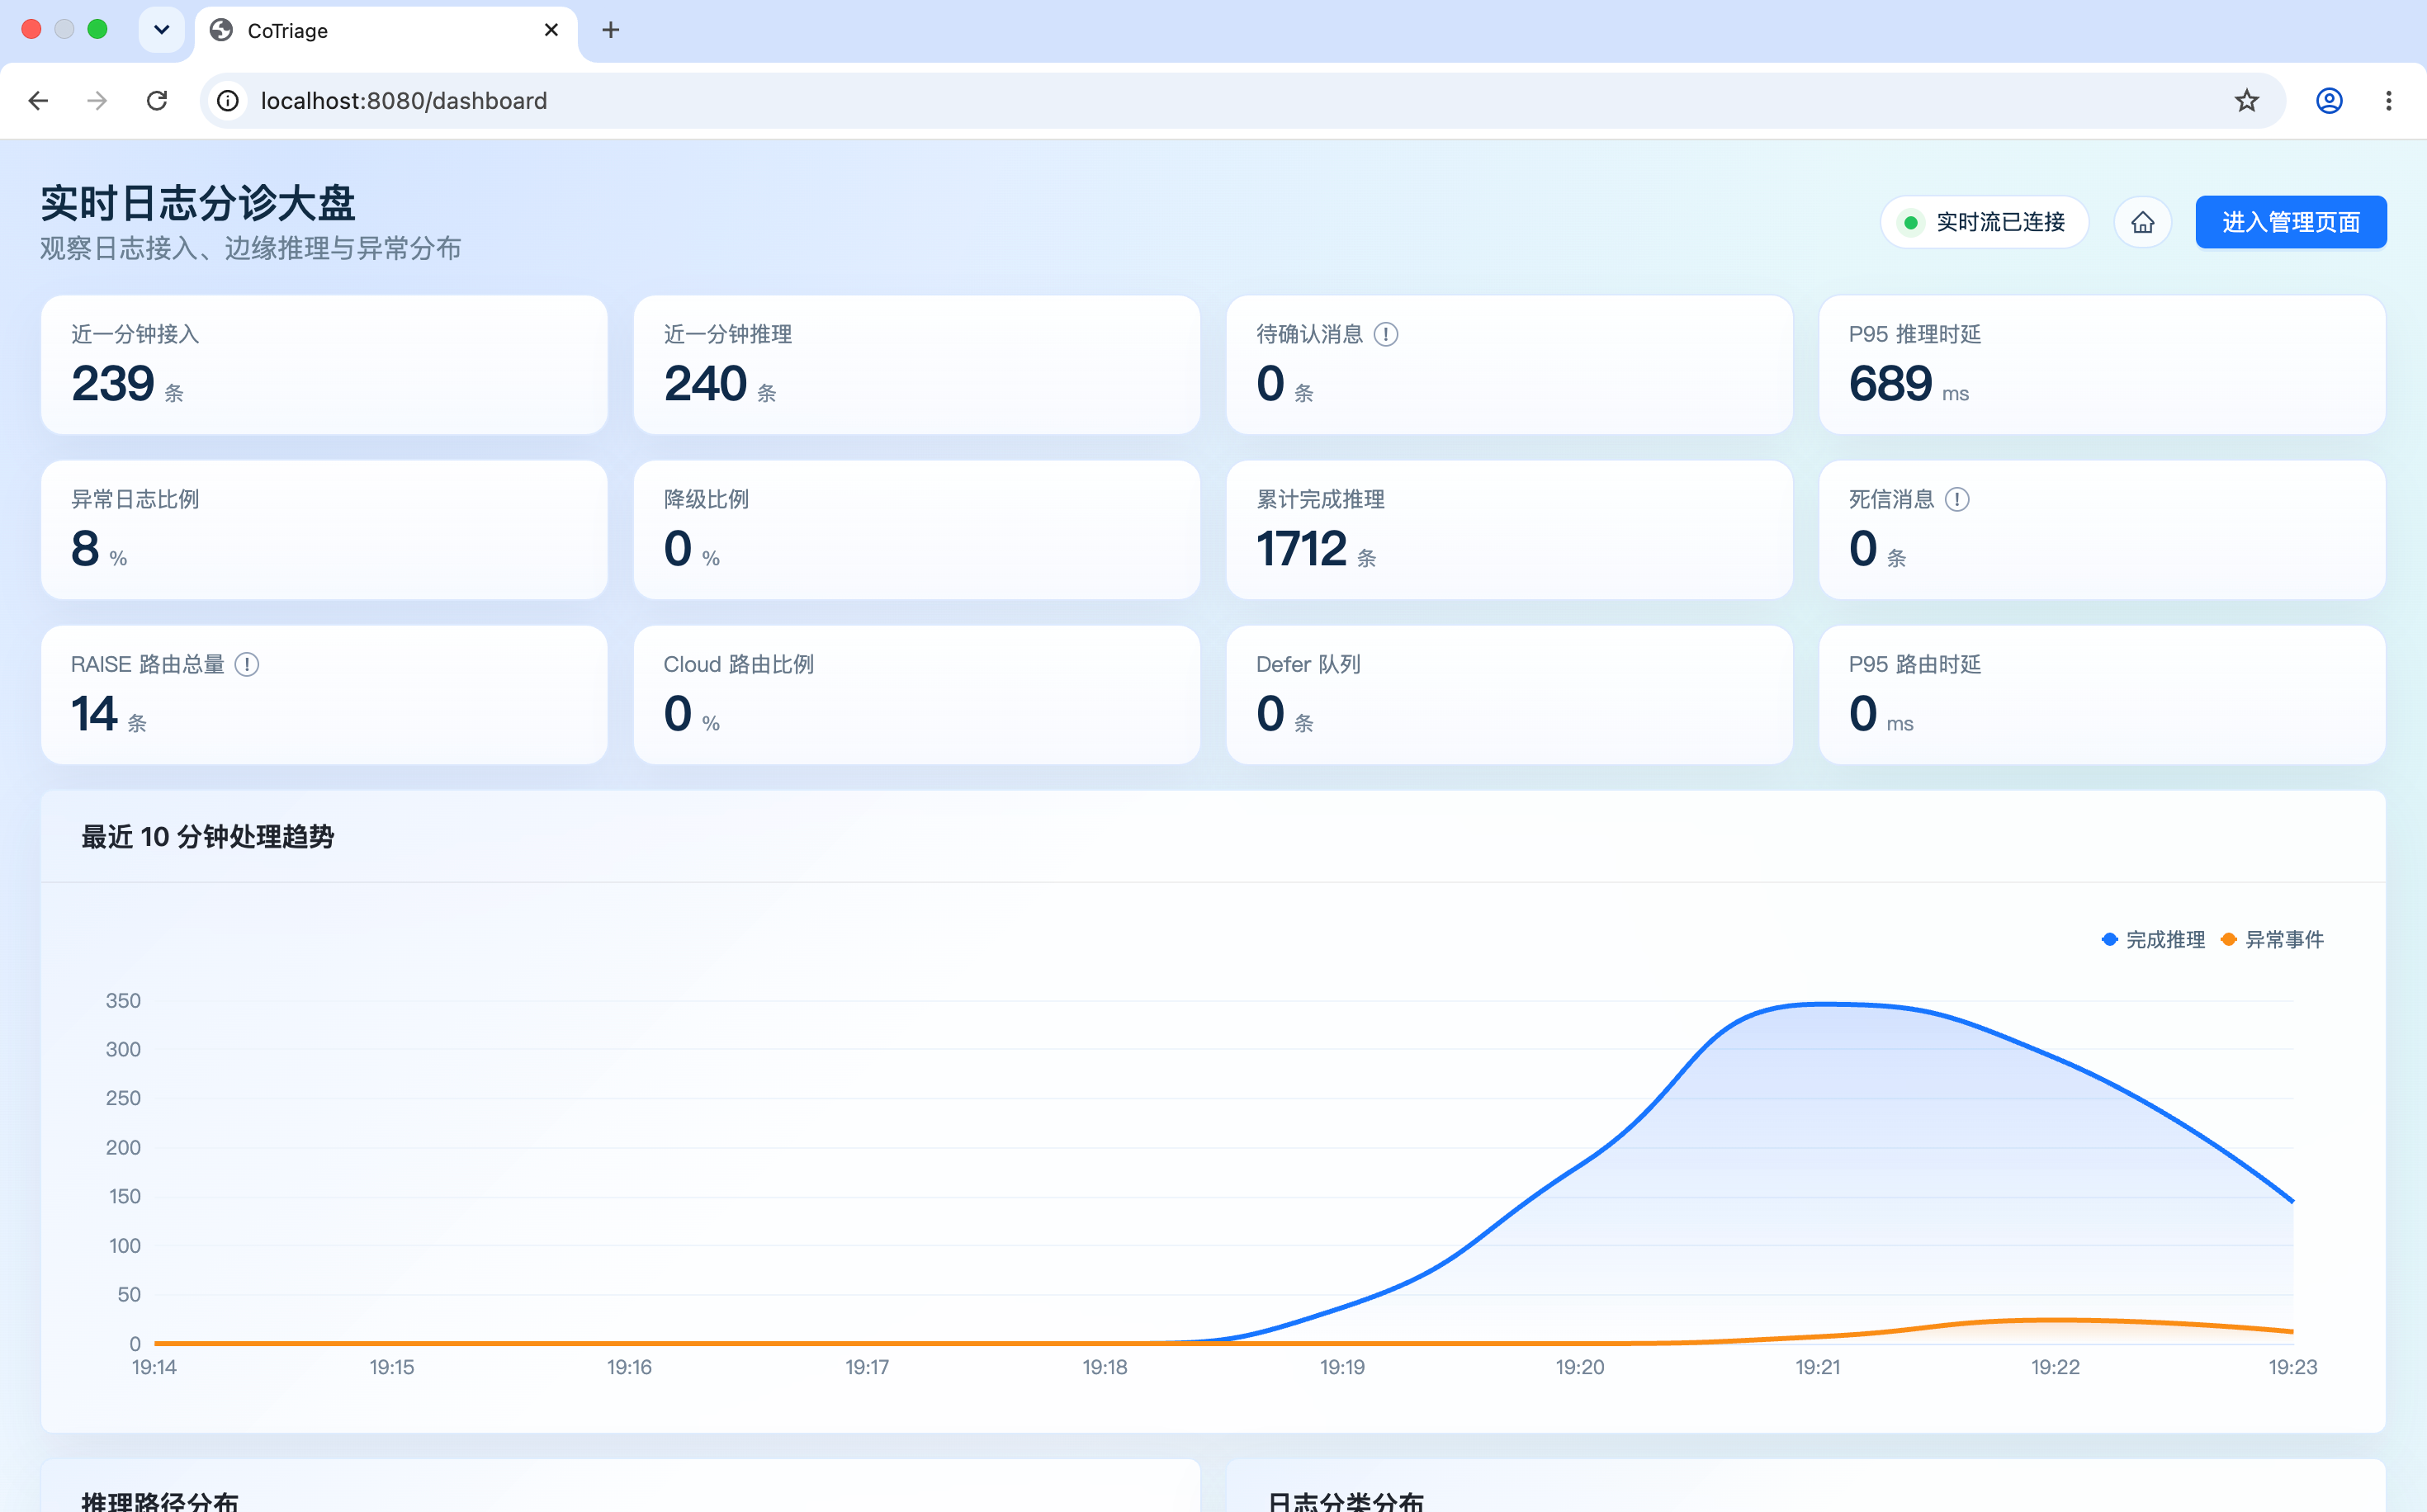
\includegraphics[width=0.98\textwidth]{figures/s-01-realtime-dashboard.png}
  \caption{REST 历史快照与 SSE 增量事件共同驱动的实时驾驶舱}
  \label{fig:realtime-dashboard}
\end{figure}

驾驶舱初始化时并行请求 summary、timeseries、abnormal-analysis、events、router summary、decisions、Outbox 和 cloud feedback，先形成一致的历史视图；随后建立 SSE 连接接收新事件，将增量数据合并到有限长度的本地数组中。连接断开时页面保留最后一次快照并进入重连状态，不会清空既有数据。用户可以暂停表格刷新，新事件暂存于缓冲区，恢复时批量合并，便于演示过程中展开某条事件而不被高频刷新打断。

页面围绕同一 \texttt{event\_id} 合并边缘事件、RAISE 决策和云端反馈。总览卡片显示接入、推理、异常、降级和路由状态；趋势图和分布图由 ECharts 响应式重绘；Outbox 区域展示状态、优先分数、尝试次数和错误；云端诊断只在根因、建议或解释字段存在时渲染相应内容，避免把不可解析占位信息展示给用户。事件表展开后显示原始日志、模板、推理证据、分阶段耗时、路由原因和云端诊断，从而把系统内部多阶段处理还原为一条可阅读的事件链。

\section{容器化部署、运维与安全实现}
\begin{figure}[htbp]
  \centering
  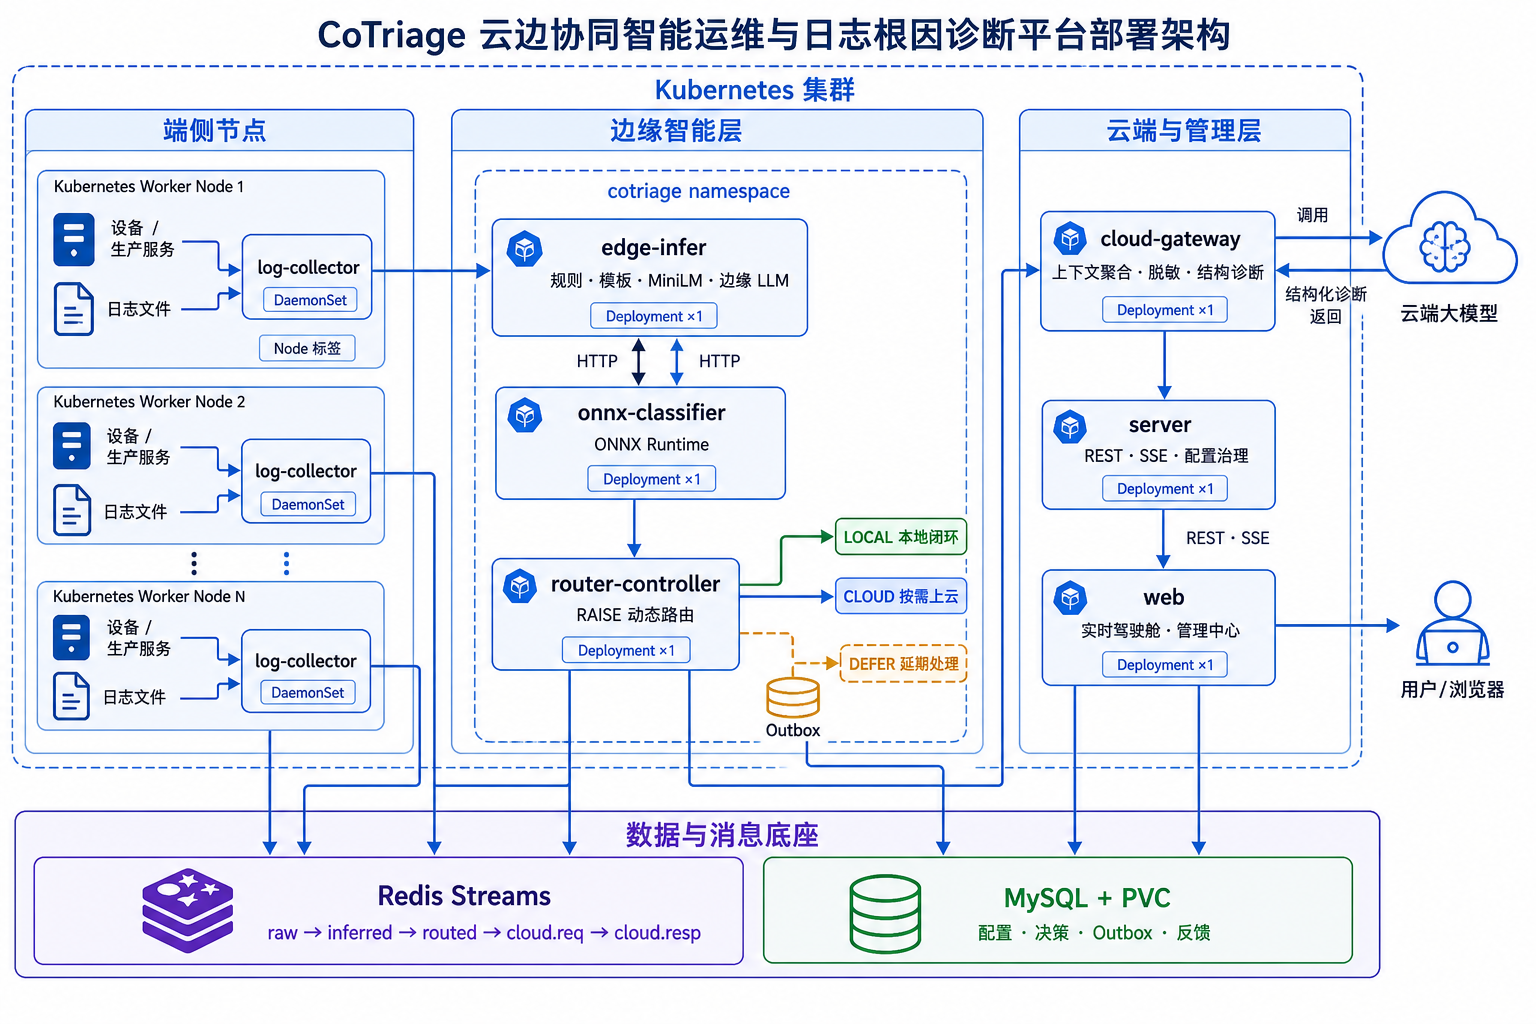
\includegraphics[width=0.98\textwidth]{figures/deployment-architecture.png}
  \caption{CoTriage 云边协同系统的 Kubernetes 部署架构}
  \label{fig:deployment-architecture}
\end{figure}

\cref{fig:deployment-architecture}给出了系统从端侧日志源、边缘智能处理到云端诊断与管理面的实际部署关系。端侧采集器以 DaemonSet 随节点部署，其余核心服务以单副本 Deployment 运行在 \texttt{cotriage} namespace；Redis Streams 承载阶段化事件流，MySQL 与 PVC 保存配置、决策、Outbox 和反馈等持久状态。云端大模型位于集群边界之外，仅由 Cloud Gateway 在路由动作选择 \texttt{CLOUD} 时按需调用。

仓库为主要服务提供独立 Dockerfile，并在 \texttt{charts/} 下维护 Kubernetes 资源。log-collector 采用 DaemonSet 贴近节点日志目录；edge-infer、onnx-classifier、router-controller、cloud-gateway、server 和 web 采用 Deployment；Redis 与 MySQL 通过 Service 暴露集群内地址并挂载 PVC。各业务组件通过 ConfigMap 或环境变量接收 Stream、超时、批次、并发和 RAISE 参数，敏感项由 Secret 或仅在进程环境中存在的变量提供。镜像可以独立构建并推送到阿里云镜像仓库，部署时限定在 \texttt{cotriage} namespace，服务间使用集群 DNS 而不是固定 Pod IP。

启动顺序首先确保 Redis、MySQL 和 ONNX 服务可用，再启动控制面、边缘推理、路由和云端网关，最后开放采集器与 Web。停止时先缩减采集入口，避免继续产生新事件，再等待或保留 Pending 与 Outbox。运行检查不仅关注 Pod 是否 Ready，还覆盖 Consumer Group Pending、Stream 长度、DLQ、MySQL 连接、Outbox 最老等待时间、云端 Provider 状态和 SSE 连接状态。组件使用 \texttt{SIGTERM} 派生的 context 结束读取循环，避免容器终止时继续接受新批次。

安全边界在实现中体现为三层：端侧通过节点标签和 ServiceAccount 最小权限识别来源；路由硬策略可禁止指定事件上云；Cloud Gateway 在构造提示词前执行脱敏和上下文裁剪。Provider 密钥不写入配置响应，管理页面只展示遮罩。对于生产环境，还需在现有基础上接入专用密钥托管、NetworkPolicy、字段级脱敏规则、访问审计和镜像签名，但这些扩展不会改变现有事件与组件接口。

综上，CoTriage 的工程实现不是若干模型接口的串联，而是一套围绕事件生命周期构建的分布式运行系统：实时路径以 Stream 和 Consumer Group 保证阶段解耦，知识与模型以版本配置实现在线治理，高价值任务以 Outbox 跨越弱网，云端结果以幂等反馈回写，控制面与驾驶舱则把内部状态转化为可操作、可解释的产品能力。

\chapter{系统运行观测}

CoTriage 的价值不只在于把日志送入不同模型，而在于能否在现场时限、诊断质量、云端开销和异常网络之间取得可解释的平衡。因此，本章围绕五个可验证问题组织观测指标：边缘侧能否及时给出首个可用判断；按需上云能否在保留诊断能力的同时减少传输和调用；云端是否真正补充了跨节点上下文与处置知识；外部服务不可用时实时主链能否继续工作；节点和日志来源增加后，协同链路是否仍保持统一。
观测指标运行支持系统用户确认组件状态、事件流量、路由分布、队列积压和单事件追踪。

\begin{table}[htbp]
  \centering
  \small
  \caption{CoTriage 的核心评估问题、测量量与证据来源}
  \label{tab:evaluation-framework}
  \begin{tabularx}{\textwidth}{>{\bfseries}p{0.17\textwidth} p{0.29\textwidth} p{0.25\textwidth} X}
    \toprule
    评估问题 & 关键测量量 & 推荐对照 & 证据来源 \\
    \midrule
    现场响应能力 & 首次可用判断 P50／P95、边缘处理时延、吞吐率 & 仅边缘、全部上云、固定阈值级联 & 事件时间戳与压测记录 \\
    感知与决策质量 & Accuracy、Macro-F1、高风险 Recall、任务完成率 & 各边缘层级及云边协同策略 & 冻结并标注的数据集 \\
    协同与通信效率 & 本地闭环率、上云比例、上传字节、Token／事件、云端调用次数 & 全量上云与固定级联 & 路由记录、网关用量和流量统计 \\
    弱网运行韧性 & 本地业务保持率、Defer 数量、Outbox 峰值、重放成功率与排空时间 & 正常、时延、丢包、断连和恢复窗口 & 故障注入记录与 Outbox 状态迁移 \\
    多节点适应性 & 节点数—吞吐曲线、端到端时延波动、相关事件冲突与收敛结果 & 不同节点规模和日志来源组合 & 设备登记、关联任务与决策审计 \\
    \bottomrule
  \end{tabularx}
\end{table}

一次事件处理包含采集、事件化、边缘推理、路由决策、可选的云端诊断以及反馈写回。由于云端诊断采用异步增强模式，系统区分“首次可用判断时延”和“完整诊断时延”：前者从采集时间起算，到边缘结果可被业务侧读取为止；后者在需要上云时继续计时，直到结构化诊断写回。这样的划分能够反映 CoTriage 的真实交付方式，也避免用较慢的云端完整生成掩盖边缘早期判断的价值。

\begin{figure}[htbp]
  \centering
  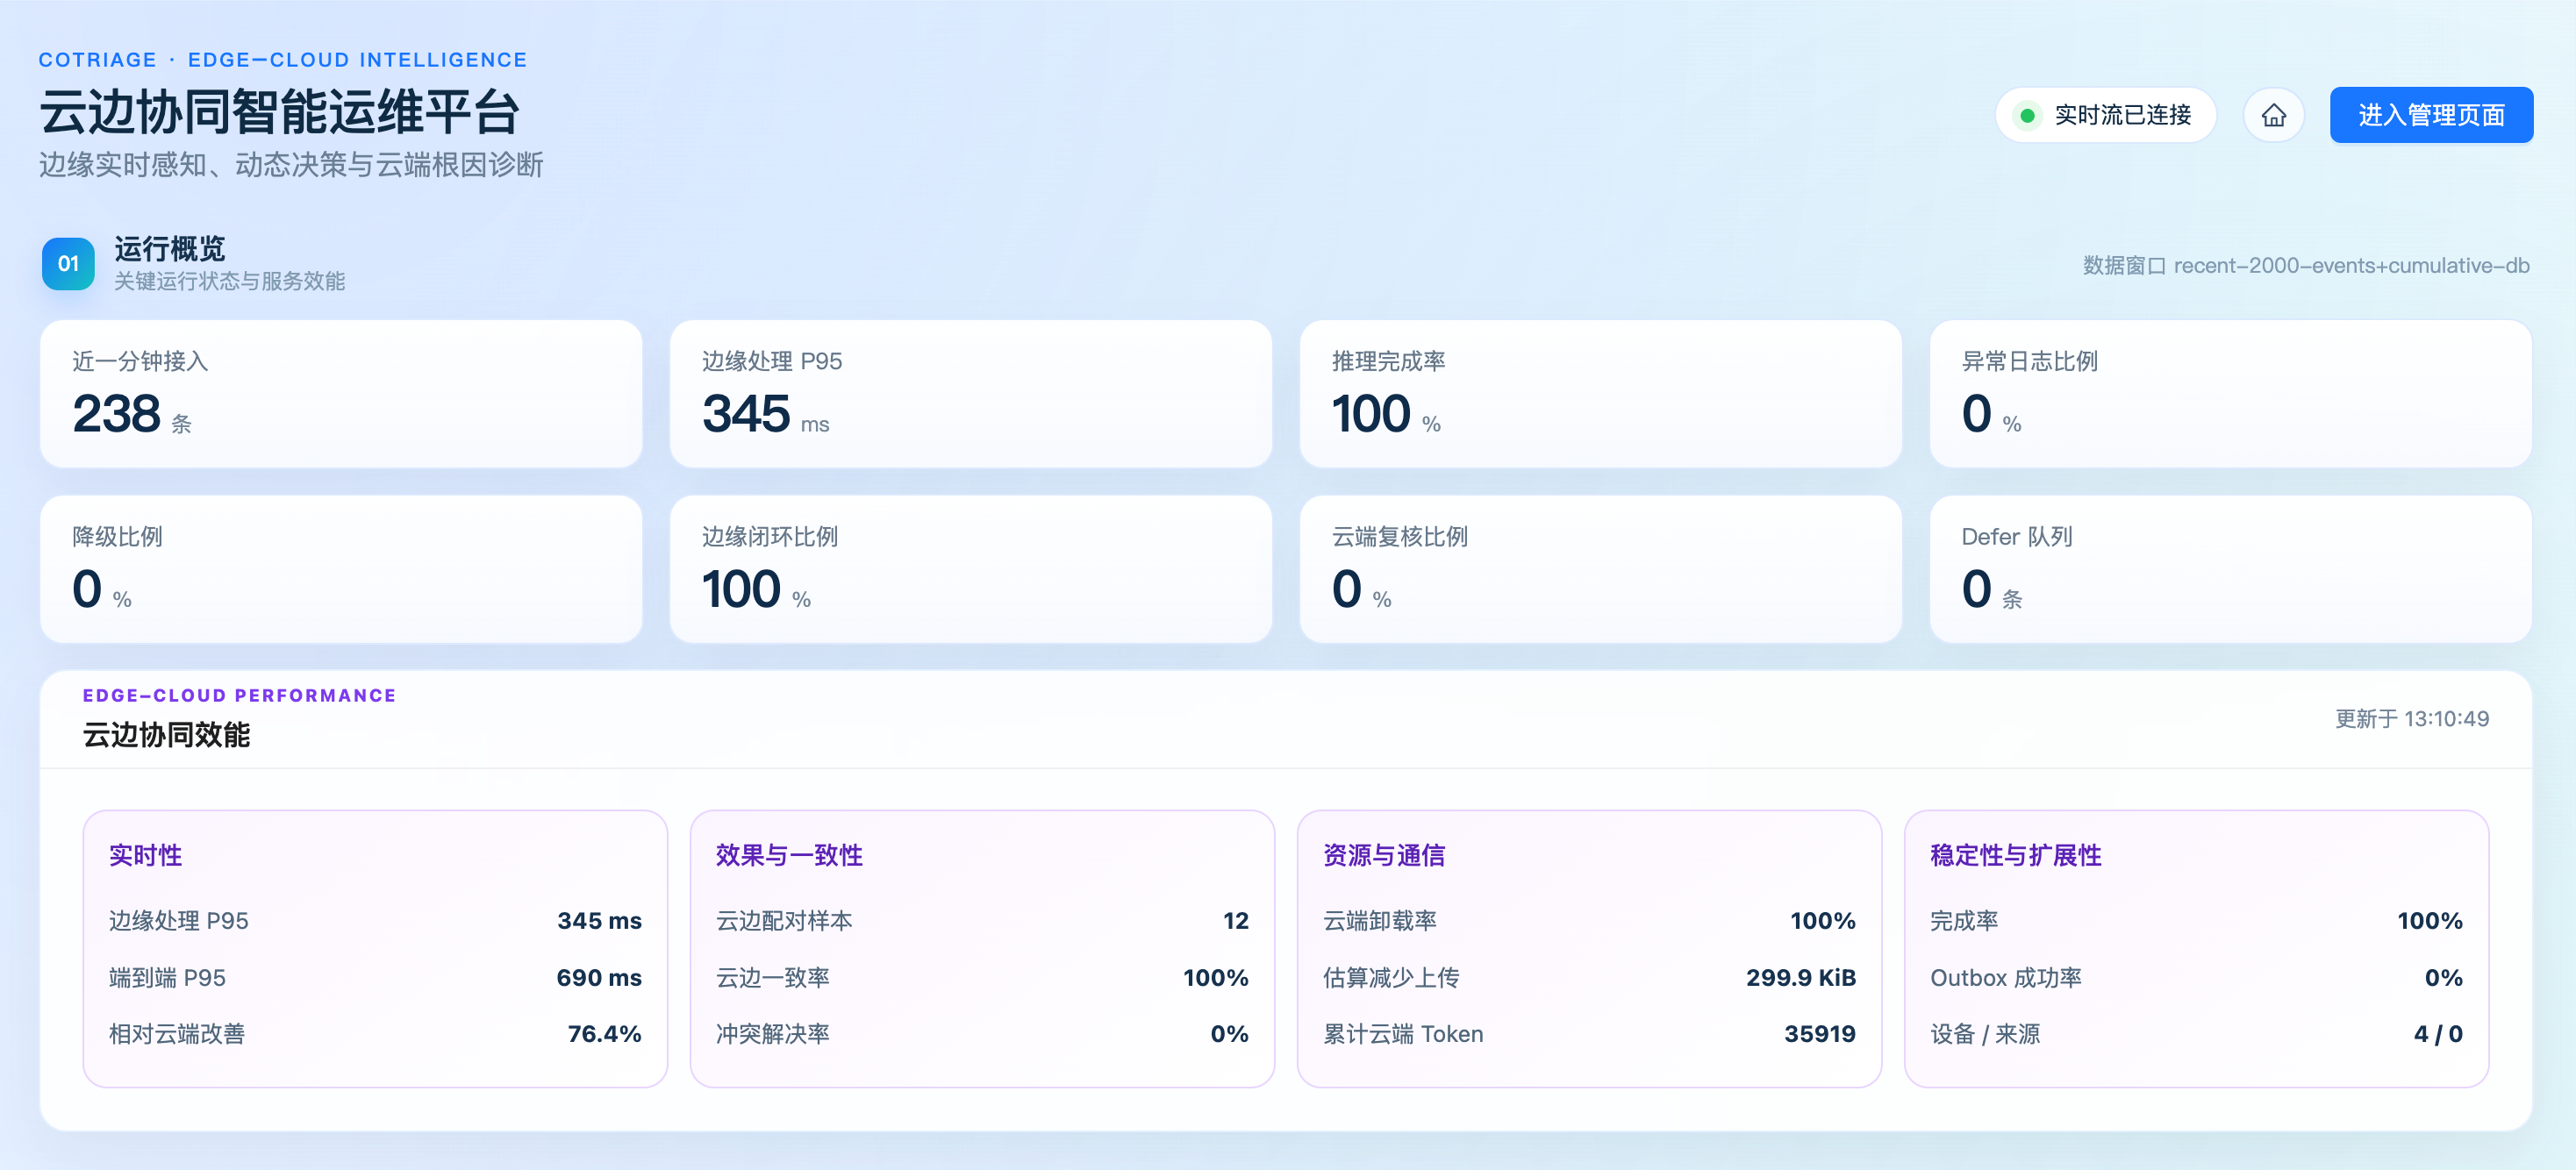
\includegraphics[width=\textwidth]{figures/s-11-competition-metrics-dashboard.png}
  \caption{CoTriage 运行质量分析界面：时延、路由、通信与可靠传输状态}
  \label{fig:runtime-quality-dashboard}
\end{figure}

\cref{fig:runtime-quality-dashboard}把接入、边缘处理、推理完成、异常、降级、云端复核和 Defer 状态组织在同一页面中，并进一步展示处理时延、边云配对、上传量、Token、Outbox 和节点接入情况。它的主要作用是把一次系统运行拆解成可追踪的阶段：运维人员既能看到总体负载与分流结构，也能沿事件标识下钻到推理路径、路由动作、云端请求和最终诊断。
\chapter{结论}

工业现场与分布式基础设施中的日志诊断，本质上不是一个单纯追求模型规模或分类精度的问题，而是一个同时受到响应时限、现场算力、网络状态、数据边界、云端成本和运维责任约束的系统决策问题。面对大量重复事件与少量复杂异常并存的长尾分布，固定规则难以持续覆盖未知模式，全量上云又会把网络往返、排队时延、调用费用和弱网不可用引入实时主链。CoTriage 从这一矛盾出发，将研究重点从“选择边缘还是云端”推进到“如何根据每个事件的价值和系统当下状态，动态分配边缘与云端能力”，由此形成面向连续日志流的云边协同故障感知与决策体系。

围绕这一目标，系统建立了端、边、云职责清晰而又能够闭环协作的总体架构。端侧贴近设备、操作系统和生产服务，负责多节点持续采集、来源标识、时间统一和事件化，使原本分散、异构、缺少共同坐标的原始日志转化为可关联、可追踪的统一事件。边缘侧承担现场实时主链，以规则、模板知识、MiniLM ONNX 轻量分类器和边缘小语言模型构成由快到慢、由确定到开放的分层推理路径，使高频已知事件能够尽早结束，困难事件能够逐级获得更强语义能力。云端不再接收无差别的原始日志洪流，而是围绕少量高风险、高不确定性事件，聚合时间邻近、设备关系、模板相似性和严重度等上下文，在受控 Token 预算内生成根因候选、处置建议和结构化解释，并将结果反馈到统一事件闭环。

云边协同能否成立，关键不在于同时部署两种模型，而在于是否存在一套能够决定“何时使用哪一侧能力”的机制。CoTriage 以 RAISE 将事件风险、不确定性、模板新颖度和历史分歧等认知因素，与网络健康、队列压力、调用预算和运维策略等运行因素纳入同一决策过程，在 \texttt{LOCAL}、\texttt{CLOUD} 和 \texttt{DEFER} 三种动作之间进行事件级选择。其中，\texttt{DEFER} 并非简单的失败回退，而是把“该事件值得获得云端增强”和“当前条件允许立即发送”两个问题主动解耦：能够在本地完成的事件继续形成现场判断，暂时无法发送的高价值任务进入 Outbox 持久化等待，网络恢复后再依据风险与到期状态重放。由此，系统把实时业务连续性与深度诊断完整性从一条相互阻塞的同步链路，转化为可以分别保障、最终汇合的双阶段过程。

在工程实现上，CoTriage 已将这一方法落实为可部署、可配置、可观测的完整软件链路。采集、边缘推理、轻量模型服务、动态路由、云端网关、可靠重放、控制服务和 Web 管理端以稳定事件、Redis Streams、HTTP 接口和持久化状态协作，各组件可以独立部署和扩展。系统不仅保存最终标签，还记录推理层级、模型与配置版本、置信度、路由动作、决策原因、云端用量、Outbox 状态及反馈结果，使每次判断能够回到具体事件、具体策略和具体运行条件。管理端进一步将实时事件流、异常态势、路由状态、云端诊断、可靠传输以及规则和模型配置组织到统一观察面中，使平台既能处理故障，也能解释故障如何被处理、分析能力为何被分配到某一侧，以及处理过程是否仍处于治理边界之内。

这种架构同时回应了工业设备与生产服务监测、分布式基础设施监测两类具有明显差异的应用需求。在工业现场，系统强调就近响应、断网可用、敏感数据最小外发和明确处置建议；在 Hadoop、ZooKeeper、Linux 与 Web 服务等分布式环境中，系统强调跨来源关联、传播链辨识和集群级上下文。两类场景共享统一事件、分层推理契约、RAISE、Outbox、云端网关和管理接口，场景差异则被限制在采集适配、领域规则、模板知识、模型配置和关联策略中。因此，新增设备协议、日志来源或业务领域时，不需要重新构造整条云边协同主链，体现出“场景适配局部化、核心链路稳定化”的系统设计思想。

从系统运行与验证结果看，CoTriage 已形成贯穿采集时间、边缘推理、路由动作、云端调用、用量统计、反馈写回和可靠传输状态的连续测量链，并完成真实部署组件之间的端到端联调。运行质量分析界面能够从总体负载下钻到单事件处理阶段，自动化执行器能够在相同输入下复现不同协同策略并归档逐样本记录。这说明系统已经由概念方案推进为可运行、可操作、可追踪和可重复验证的工程原型。更重要的是，平台明确区分带真值的离线评测、受控条件下的对照实验和线上运行观测，使准确率、时延、通信量、弱网保持与多节点一致性等结论能够对应到各自的数据来源和统计边界，而不依赖孤立截图或缺少分母的百分比。

CoTriage 所探索的并不仅是一种日志分类流程，而是一种面向受限环境的分布式智能组织方式：把确定性知识和快速判断尽可能下沉到现场，把稀缺而强大的云端认知能力集中到真正需要的事件，把暂时不可用的外部能力转化为可管理、可恢复的延期任务，再以统一事件和反馈机制连接感知、决策与治理。这样，边缘不再只是云端模型的前置过滤器，云端也不再是所有数据的默认终点；二者分别承担符合自身信息范围、资源条件和时间约束的任务，并通过动态路由形成随事件和环境变化而调整的协作关系。

面向未来，随着边缘模型、云端大模型和工业知识库持续演进，这套体系可以进一步吸收更丰富的时序关联、拓扑依赖和反馈学习能力，也可以与企业现有告警、工单、知识库和设备控制平台衔接，形成从异常发现、根因诊断到处置协同的更完整闭环。但无论模型和场景如何变化，CoTriage 所确立的基本原则保持不变：现场必须拥有不依赖云端的首要判断能力，高价值复杂事件应当按需获得更强认知资源，网络波动不应使重要任务静默丢失，任何自动决策都应留下可解释、可审计、可回滚的依据。


\clearpage
\printbibliography[heading=bibintoc,title={参考文献}]

\end{document}
